%%%%%%%%%%%%%%%%%%%%%%%%%%%%%%%%%%%%%%%%%%%%%%%%%%%%%%%%%%%%%%%%%%%%%%%%%
%%
%%  D I S S E R T A T I O N
%%
%%  Sergio A. de Carvalho Jr.
%%
%%%%%%%%%%%%%%%%%%%%%%%%%%%%%%%%%%%%%%%%%%%%%%%%%%%%%%%%%%%%%%%%%%%%%%%%%
\documentclass[12pt,pagesize,a4paper,BCOR1cm,DIV13,headsepline,cleardoubleplain,chapterprefix,halfparskip,pointlessnumbers,tablecaptionabove]{scrbook}
\usepackage{setspace}
\usepackage{amsmath,amssymb,amsthm,amsfonts}
\usepackage{latexsym}
\usepackage[american]{babel} 
\usepackage[round]{natbib}
\usepackage{longtable}
\usepackage{graphicx}\graphicspath{{./figures/}}
\usepackage{url}
\usepackage{bbm}
\usepackage{float}

%%%%%%%%%%%%%%%%%%%%%%%%%%%%%%%%%%%%%%%%%%%%%%%%%%%%%%%%%%%%%%%%%%%%%%%%%
% Further document formatting instructions
%%%%%%%%%%%%%%%%%%%%%%%%%%%%%%%%%%%%%%%%%%%%%%%%%%%%%%%%%%%%%%%%%%%%%%%%%
\setcapindent{1em}
\addtokomafont{caption}{\small}
\setkomafont{captionlabel}{\sffamily\bfseries}

%%%%%%%%%%%%%%%%%%%%%%%%%%%%%%%%%%%%%%%%%%%%%%%%%%%%%%%%%%%%%%%%%%%%%%%%%
% New environments and commands; hyphenation exceptions
%%%%%%%%%%%%%%%%%%%%%%%%%%%%%%%%%%%%%%%%%%%%%%%%%%%%%%%%%%%%%%%%%%%%%%%%%
%%%%%%%%%%%%%%%%%%%%%%%%%%%%%%%%%%%%%%%%%%%%%%%%%%%%%%%%%%%%%%%%%%%%%%
%% A hyphen that allows further hyphenation of a word
%%%%%%%%%%%%%%%%%%%%%%%%%%%%%%%%%%%%%%%%%%%%%%%%%%%%%%%%%%%%%%%%%%%%%%
\def\hyph{-\penalty0\hskip0pt\relax}

%%%%%%%%%%%%%%%%%%%%%%%%%%%%%%%%%%%%%%%%%%%%%%%%%%%%%%%%%%%%%%%%%%%%%%
%% Algorithm names
%%%%%%%%%%%%%%%%%%%%%%%%%%%%%%%%%%%%%%%%%%%%%%%%%%%%%%%%%%%%%%%%%%%%%%
\newcommand{\Greedyplus}{Greedy+}

%%%%%%%%%%%%%%%%%%%%%%%%%%%%%%%%%%%%%%%%%%%%%%%%%%%%%%%%%%%%%%%%%%%%%%
%% AMS definitions
%%%%%%%%%%%%%%%%%%%%%%%%%%%%%%%%%%%%%%%%%%%%%%%%%%%%%%%%%%%%%%%%%%%%%%
\theoremstyle{definition}
\newtheorem{problem}{Problem}
\newtheorem{definition}{Definition}[chapter]
\newtheorem{claim}[definition]{Claim}
\newtheorem{example}[definition]{Example}
\newtheorem{corollary}[definition]{Corollary}

\theoremstyle{plain}
\newtheorem{lemma}[definition]{Lemma}
\newtheorem{theorem}[definition]{Theorem}

%%%%%%%%%%%%%%%%%%%%%%%%%%%%%%%%%%%%%%%%%%%%%%%%%%%%%%%%%%%%%%%%%%%%%%
%% Float for displaying algorithms
%%%%%%%%%%%%%%%%%%%%%%%%%%%%%%%%%%%%%%%%%%%%%%%%%%%%%%%%%%%%%%%%%%%%%%
\floatstyle{ruled}
\floatname{algorithm}{Algorithm}
\newfloat{algorithm}{t}{}

%%%%%%%%%%%%%%%%%%%%%%%%%%%%%%%%%%%%%%%%%%%%%%%%%%%%%%%%%%%%%%%%%%%%%%%%%
% New commands
%%%%%%%%%%%%%%%%%%%%%%%%%%%%%%%%%%%%%%%%%%%%%%%%%%%%%%%%%%%%%%%%%%%%%%%%%

% Ignore, forcebreak, ...
\newcommand{\ignore}[1]{}
\newcommand{\forcebreak}{\nopagebreak\mbox{ }\\[-3ex]\nopagebreak}
\newcommand{\eop}{\hfill$\bullet$}

% Sets
\newcommand{\setR}{\mathbb{R}}

% Nucleotides
\newcommand{\DNA}{\text{DNA}}
\newcommand{\RNA}{\text{RNA}}
\newcommand{\tA}{\text{\small{\tt A}}}
\newcommand{\tC}{\text{\small{\tt C}}}
\newcommand{\tG}{\text{\small{\tt G}}}
\newcommand{\tN}{\text{\small{\tt N}}}
\newcommand{\tT}{\text{\small{\tt T}}}
\newcommand{\tU}{\text{\small{\tt U}}}
\newcommand{\tX}{\text{\small{\tt X}}}
\newcommand{\Seq}[1]{{\text{\small{\tt{#1}}}}}
\newcommand{\Nucs}[1]{{\text{\small{\tt{#1}}}}}
\newcommand{\emptyseq}{\epsilon}
\newcommand{\sep}{\text{\ttfamily \$}}
\newcommand{\wild}{\text{\ttfamily X}}
\newcommand{\SigmaX}{(\Sigma\cup\{\wild\})}

% Probability
\newcommand{\Erw}{\mathbb{E}}
\newcommand{\Var}{\text{Var}}
\newcommand{\R}{\mathbb{R}}
\newcommand{\Prob}{\mathbb{P}}
\newcommand{\Probhat}{\hat{\mathbb{P}}}
%%\newcommand{\Ind}[1]{\ensuremath{{\mathbb{I}}_{\{#1\}} }}
\newcommand{\Ind}[1]{\mathbbm{1}_{\{{#1}\}}}
\newcommand{\Eins}{{\mathbb{I}}}
\newcommand{\given}{\,|\,}

% Cal Letters
\newcommand{\CalA}{{\mathcal{A}}}
\newcommand{\CalB}{{\mathcal{B}}}
\newcommand{\CalC}{{\mathcal{C}}}
\newcommand{\CalD}{{\mathcal{D}}}
\newcommand{\CalE}{{\mathcal{E}}}
\newcommand{\CalF}{{\mathcal{F}}}
\newcommand{\CalG}{{\mathcal{G}}}
\newcommand{\CalL}{{\mathcal{L}}}
\newcommand{\CalM}{{\mathcal{M}}}
\newcommand{\CalN}{{\mathcal{N}}}
\newcommand{\CalP}{{\mathcal{P}}}
\newcommand{\CalQ}{{\mathcal{Q}}}
\newcommand{\CalS}{{\mathcal{S}}}
\newcommand{\CalT}{{\mathcal{T}}}
\newcommand{\CalU}{{\mathcal{U}}}
\newcommand{\CalX}{{\mathcal{X}}}
\newcommand{\CalY}{{\mathcal{Y}}}

% Algorithms
\newcommand{\aname}[1]{\textsc{#1}}
\newcommand{\atab}{\makebox[6ex]{}}
\newcommand{\MFOLD}{\aname{Mfold}}

% Binomial-like coefficients
\newcommand{\schoose}[2]{{\genfrac{(}{)}{0pt}{}{{#1}}{{#2}}}}
\newcommand{\ssubset}[2]{{\genfrac{\{}{\}}{0pt}{}{{#1}}{{#2}}}}
\newcommand{\scycle}[2]{{\genfrac{[}{]}{0pt}{}{{#1}}{{#2}}}}
\newcommand{\falling}[2]{{{#1}^{\underline{#2}}}}

% Other Math
\newcommand{\mathand}{{\text{ and }}}
\newcommand{\diag}{{\text{diag}}}
\newcommand{\N}{{\mathbb{N}}}

\newcommand{\eps}{\varepsilon}
\newcommand{\sig}{\varsigma}
\newcommand{\vphi}{\varphi}
\newcommand{\valpha}{{\underline{\alpha}}}
\newcommand{\vbeta}{{\underline{\beta}}}

% Bars and Hats
\newcommand{\betabar}{{\overline{\beta}}}
\newcommand{\lambdabar}{{\overline{\lambda}}}
\newcommand{\nbar}{{\overline{n}}}
\newcommand{\Thetabar}{\ensuremath{\overline{\Theta}}}
\newcommand{\Bbar}{{\overline{B}}}
\newcommand{\Ubar}{{\overline{U}}}
\newcommand{\ubar}{{\overline{u}}}
\newcommand{\vbar}{{\overline{v}}}
\newcommand{\xbar}{\ensuremath{\overline{x}}}
\newcommand{\Xbar}{\ensuremath{\overline{X}}}
\newcommand{\ybar}{{\overline{y}}}
\newcommand{\Phihat}{{\ensuremath{\hat{\Phi}}}}

%% (R)
%% \newcommand{\textR}{${}^\text{\textregistered}$}
\newcommand{\textR}{\raisebox{.6ex}{\scriptsize \textregistered}}

%% Na+, TM, *C, A, differential d.
\newcommand{\Naplus}{{\ensuremath{\text{Na}^+}}}
\newcommand{\TM}{T_\text{M}}
\newcommand{\degC}{\ensuremath{{}^\circ\text{C}}}
\newcommand{\Angstrom}{\text{\AA}}
\newcommand{\diff}{\,\text{d}}
\newcommand{\Dstd}[1]{\Delta{#1}^\circ}
\newcommand{\stdm}[1]{{#1}^\circ_\text{m}}
\newcommand{\Drstd}[1]{\Delta_\text{r}{#1}^\circ}
\newcommand{\Dr}[1]{\Delta_\text{r}{#1}}
\newcommand{\conceq}[1]{[{#1}]_\text{eq}}
\newcommand{\fd}[1]{$5'$-\Nucs{#1}-$3'$}
\newcommand{\rfd}[1]{r($5'$-\Nucs{#1}-$3'$)}
\newcommand{\dfd}[1]{d($5'$-\Nucs{#1}-$3'$)}

%% Strings, lcf and so on 
\newcommand{\substring}{\lhd}
\newcommand{\suf}[2]{{#1}_{(#2)}}

\newcommand{\lcf}{\ensuremath{\text{\upshape lcf}}}
\newcommand{\lcfe}{\ensuremath{\text{\upshape lcf}^1}}
\newcommand{\lcfvec}{\ensuremath{\text{\upshape LCF}}}
\newcommand{\lcfstat}{\ensuremath{\text{\upshape LCFS}}}

\newcommand{\lcpr}{\text{lcp}}  %% lcpr = lcp in roman font

\newcommand{\ms}{\text{\upshape ms}}
\newcommand{\mse}{\text{\upshape ms}^1}

\newcommand{\Romin}{{R^0_{\min}}}
\newcommand{\Remin}{{R^1_{\min}}}
\newcommand{\Rmax}{{R_{\max}}}

\newcommand{\pos}{\text{\upshape\ttfamily pos}}
\newcommand{\rank}{\text{\upshape\ttfamily rank}}
\newcommand{\cl}{\text{\upshape\ttfamily cl}}
\newcommand{\bck}{\text{\upshape\ttfamily bck}}
\newcommand{\lcp}{\text{\upshape\ttfamily lcp}}
\newcommand{\MS}{\text{\upshape\ttfamily MS}}
\newcommand{\MSe}{{\text{\upshape\ttfamily MS}^1}}
\newcommand{\qcode}[1]{\langle{#1}\rangle}

\newcommand{\csms}{\text{\upshape csms}}
\newcommand{\CSMS}{{\text{\upshape\ttfamily CSMS}}}

\newcommand{\Lo}{{L^\circ}}

%% Other Stuff
\newcommand{\steep}{\text{\textit{drop}}}
\newcommand{\clust}{\mathcal{B}}

%% Matrices
\newcommand{\cond}{\ensuremath{\text{\upshape cond}}}
\newcommand{\Rank}{\ensuremath{\text{\upshape rank}}}
\newcommand{\scond}{\ensuremath{\text{\upshape cond}_\text{\upshape{s}}}}
\newcommand{\tp}{\ensuremath{{}^\text{\sffamily\upshape T}}}
\newcommand{\MR}[2]{\ensuremath{\setR^{{#1}\times{#2}}}}
\newcommand{\Id}[1]{\ensuremath{\text{\upshape I}}_{#1}}
\newcommand{\eqmin}{\ensuremath{\simeq}}
\newcommand{\nm}[1]{\ensuremath{\| {#1} \|}}
\newcommand{\expm}{\ensuremath{\text{\upshape expm}}}

%% NonUnique
\newcommand{\mcov}{\mathcal{M}}
\newcommand{\acov}{\mathcal{A}}
\newcommand{\cmin}{\gamma}
\newcommand{\hmin}{\sigma}
\newcommand{\SDiff}[2]{{#1}\Delta{#2}}
\newcommand{\Separate}{\text{\textsc{Separate}}}
\newcommand{\ddpvec}{\begin{pmatrix}\delta\\\delta^+\end{pmatrix}}
\newcommand{\ddpvectp}{\begin{pmatrix}\delta\\\delta^+\end{pmatrix}^\text{\sffamily\upshape T}}
\newcommand{\hhpvec}[1]{\begin{pmatrix}h_{#1}\\h^+_{#1}\end{pmatrix}}
\newcommand{\zzpvec}[1]{\begin{pmatrix}z^{#1}\\z^{+,{#1}}\end{pmatrix}}

\hyphenation{phyco-erythrin strept-avidin oligo-nu-cleo-tide
Af-fy-met-rix tran-script hy-bri-di-za-tion cRNAs cRNA}

%%%%%%%%%%%%%%%%%%%%%%%%%%%%%%%%%%%%%%%%%%%%%%%%%%%%%%%%%%%%%%%%%%%%%%%%%
% Date handed-in
%%%%%%%%%%%%%%%%%%%%%%%%%%%%%%%%%%%%%%%%%%%%%%%%%%%%%%%%%%%%%%%%%%%%%%%%%
\newcommand{\abgabemonat}{Februar~2007}
\newcommand{\handinmonth}{February~2007}

%%%%%%%%%%%%%%%%%%%%%%%%%%%%%%%%%%%%%%%%%%%%%%%%%%%%%%%%%%%%%%%%%%%%%%%%%
% Beginning of document
%%%%%%%%%%%%%%%%%%%%%%%%%%%%%%%%%%%%%%%%%%%%%%%%%%%%%%%%%%%%%%%%%%%%%%%%%
\begin{document}
\selectlanguage{\american}
\frontmatter\pagestyle{plain}

%%%%%%%%%%%%%%%%%%%%%%%%%%%%%%%%%%%%%%%%%%%%%%%%%%%%%%%%%%%%%%%%%%%%%%%%%
%% Title pages
%%%%%%%%%%%%%%%%%%%%%%%%%%%%%%%%%%%%%%%%%%%%%%%%%%%%%%%%%%%%%%%%%%%%%%%%%
\title{Algorithms for Improving the Design and Production of
  Oligonucleotide Microarrays}
\author{S\'ergio Anibal de Carvalho Junior}
\date{\abgabemonat}
\publishers{\large{
  Dissertation\\
  zur Erlangung des akademischen Grades\\
  eines Doktors der Naturwissenschaften\\
  (Doctor rerum naturalium)\\
  ~\\
  an der Technischen Fakult\"at\\
  der Universit\"at Bielefeld\\
  ~\\
  ~\\
  Betreuer:\\
  Dr.~rer.~nat.~Sven Rahmann\\
  Prof.~Dr.~rer.~nat.~Jens Stoye\\
  ~\\
}}
%\lowertitleback{
%  1. Referee: Prof.~Dr.~Jens~Stoye\\
%  2. Referee: Dr.~Sven~Rahmann\\[2ex]
%}
%% \dedication{}
\maketitle[-1]

%%%%%%%%%%%%%%%%%%%%%%%%%%%%%%%%%%%%%%%%%%%%%%%%%%%%%%%%%%%%%%%%%%%%%%%%%
%% Front matter
%%%%%%%%%%%%%%%%%%%%%%%%%%%%%%%%%%%%%%%%%%%%%%%%%%%%%%%%%%%%%%%%%%%%%%%%%
\clearpage
\setcounter{tocdepth}{1}
%%\listoffigures
%%\listoftables
%%%%%%%%%%%%%%%%%%%%%%%%%%%%%%%%%%%%%%%%%%%%%%%%%%%%%%%%%%%%%%%%%%%%%%%%%%%%%%%%
\chapter*{Foreword}
\addcontentsline{toc}{chapter}{Foreword}
%%%%%%%%%%%%%%%%%%%%%%%%%%%%%%%%%%%%%%%%%%%%%%%%%%%%%%%%%%%%%%%%%%%%%%%%%%%%%%%%

Microarrays are a ubiquitous tool in molecular biology with a wide range of
applications on a whole-genome scale including high-throughput gene expression
analysis, genotyping, and resequencing. Although several different microarray
platforms exist, we focus on high-density oligonucleotide arrays, sometimes
called DNA chips. One of the advantages of higher density arrays is that they
allow the simultaneous measurement of the expression of several thousand genes
at once, possibly covering all genes of a species in a single experiment.

Oligonucleotide microarrays consist of short DNA molecules, called
\emph{probes}, affixed or synthesized at specific locations of a solid support.
Probes are built, nucleotide-by-nucleotide, by a light-directed combinatorial
chemistry. Because of the natural properties of light, the quality of a
microarray can be compromised if the physical arrangement of the probes on the
array and their synthesis schedule are not carefully designed. This thesis is
mainly concerned with the problem of designing the layout of a microarray in
such a way that the incidence of the \emph{unintended illumination problem} is
reduced. We call it the \emph{microarray layout problem} (MLP), using the term
\emph{layout} to refer to where and how the probes are synthesized on the array,
i.e., their arrangement and their \emph{embeddings}.

In the first chapter of this thesis, we briefly review the role of microarrays
in analyzing complex genetic information. We then describe the technology
currently employed in the production of high-density microarrays as well as the
problems that arise during manufacturing. In Chapter \ref{ch:mlp}, we give a
formal definition to the microarray layout problem and describe in detail two
quality measures that are used to evaluate a given layout. Finding an optimal
layout with respect to any of these two measures seems unlikely, even for very
small arrays. As we shall see in Chapter \ref{ch:qap}, the MLP can be modeled as
a quadratic assignment problem (QAP), a classical combinatorial optimization
problem that is notoriously hard to solve in practice, which gives further
indication that the MLP is, in fact, a hard problem. For this reason, the layout
problem is usually approached in several ``phases'' with a range of heuristic
algorithms.

The \emph{placement} phase is the subject of Chapter \ref{ch:placement}.
Traditionally, this phase consists of fixing an embedding for all probes and
finding an arrangement minimizing a given cost function. We describe several
known placement algorithms with an emphasis on methods that can be used to
design large arrays. A new algorithm, called Greedy, is also presented. One of
the reason why we show the relation between the MLP and the QAP is that we can
now use QAP techniques as placement algorithms. This is interesting because
there is a rich literature on methods for solving the QAP. In Chapter
\ref{ch:qap}, we also show the results of using one QAP heuristic to design
small artificial chips, and discuss how this approach can be applied to larger
microarrays.

Chapter \ref{ch:reembed} focuses on the \emph{re-embedding} phase that usually
follows the placement. In this phase, one attempts to further improve the layout
by finding a different embedding of the probes without changing their location
on the chip. Again, we review all known re-embedding algorithms, describring the
most successful ones in detail. We also introduce a new algorithm, called
Priority re-embedding.

In the last decade, commercial microarrays have grown from a few thousands to
more than a million probe sequences on a single chip. Many placement algorithms
are unable to deal with such large arrays because of their non-linear time and
space complexities. For this reason, the layout problem is sometimes broken into
smaller sub-problem by a \emph{partitioning} algorithm. This is the focus of
Chapter \ref{ch:part}, where we present an extensive practical evaluation of
existing algorithms and show how the partitioning phase can improve solution
quality and reduce running time.

In Chapter \ref{ch:merge}, we discuss the disadvantages of the tradional ``place
and re-embed'' approach to the layout problem. We then propose a new algorithm,
called \Greedyplus, that for the first merges the placement and re-embedding
phases into a single one. Our results show that \Greedyplus indeed outperforms
all known placement algorithms.

In Chapter \ref{ch:affy}, we present a pioneering analysis and evaluation of the
layout of several GeneChip arrays, considered the industry standard in terms of
high-density oligonucleotide microarrays. We describe in detail design decisions
that might affect the quality of these commercially available arrays. We then
use some of the algorithms presented in earlier chapters to propose alternative
layouts for two of the latest generation of GeneChip arrays, showing how the
risk of the unintended illumination problem can be reduced.

Another problem related to the production of microarrays is the problem of
finding the shortest synthesis schedule for a given set of probes, which we
refer to as the \emph{shortest deposition sequence problem} (SDSP). The SDSP is
an instance of the shortest common supersequence problem (SCSP), a classical
problem in computer science that is known to be NP-complete even under various
restrictions. Several existing heuristics are able to find good approximate
solutions for the SCSP, but, in Chapter \ref{ch:scs}, we investigate the
feasibility of finding \emph{the shortest} deposition sequence for currently
available oligonucleotide microarrays. Chapter \ref{ch:discuss} concludes this
thesis with a short discussion about the presented results.

\paragraph{Publications.}
Parts of this thesis have been published in advance. The conflict index model
for evaluating a microarray layout (Chapter \ref{ch:mlp}) and the Pivot
Partitioning algorithm (Section \ref{sec:part_pp}) were first presented at the
Workshop on Algorithms in Bioinformatics (WABI), in Z\"urich
\citep{Carvalho2006}. The conflict index model was also presented, together with
the QAP formulation of the microarray layout problem (Chapter \ref{ch:qap}), at
the German Conference on Bioinformatics (GCB) in T\"ubingen
\citep{Carvalho2006a}. The work on the shortest common supersequence (Chapter
\ref{ch:scs}) was first published as a technical report at the Faculty of
Technology of Bielefeld University \citep{Carvalho2005}. Finally, a book chapter
containing a more accessible description of the microarray layout problem and of
most algorithms presented here is expected to appear in late 2007
\citep{Carvalho2007}.

This thesis also contains previously unpublished material, namely:
\begin{itemize}
\item the Greedy placement algorithm (Section \ref{sec:placement_greedy}) that
      outperforms previous algorithms in terms of conflict index minimization;
\item the Priority re-embedding algorithm (Section \ref{sec:reembed_priority})
      that achieves marginal improvements compared to the best known algorithms;
\item analysis of the layout of several commercially available GeneChip arrays
      with respect to the defined evaluation criteria (Chapter \ref{ch:affy}).
\end{itemize}

\paragraph{Acknowledgments.}
This work was carried out while I was a member of the Junior research group
(recently-renamed) Computational Methods for Emerging Technologies (COMET), which
is part of the AG Genominformatik led by Prof.~Jens Stoye. I thank all present
and former colleagues as well as students of the International NRW Graduate
School in Bioinformatics and Genome Research and the Graduiertenkolleg
Bioinformatik, of which I am also a member, for the nice research atmosphere I
found in Bielefeld, and for an enjoyable time I had in the last three years.

Special thanks go to Dr.~Sven Rahmann for suggesting the topic and for the
opportunity to work under his supervision. This work owes much to his expertise.
Whenever I write ``we'' in this thesis, I mean ``Sven and I''. On several
occasions, the support of the Bioinformatics Resource facility (BRF) at the
CeBiTec (Center for BioTechnology) was crucial to the success of this work,
and I cannot thank them enough for their help. Epameinondas Fritzilas,
Ferdinando Cicalese, Francisco Pereira Lobo, Jos\'e Augusto Amgarten Quitzau,
and Klaus-Bernd Sch \"urmann read early drafts of several chapters of this
thesis and helped to improve them in many ways. I would also like to thank
Dr.~Peter Hahn and Chris MacPhee for working on several QAP instances of
Chapter~\ref{ch:qap} and for helpful discussions.

\vspace*{6ex}
S\'ergio A. de Carvalho Jr.\hfill Bielefeld, \handindate

%%%%%%%%%%%%%%%%%%%%%%%%%%%%%%%%%%%%%%%%%%%%%%%%%%%%%%%%%%%%%%%%%%%%%%%%%%%%%%%%%%
\chapter*{Danke sch\"on!}
\addcontentsline{toc}{chapter}{Danke sch\"on!}
%%%%%%%%%%%%%%%%%%%%%%%%%%%%%%%%%%%%%%%%%%%%%%%%%%%%%%%%%%%%%%%%%%%%%%%%%%%%%%%%

Danke sch\"on!
%%\chapter{Abbreviations and Notation}
\label{ch:notation}

%% %%%%%%%%%%%%%%%%%%%%%%%%%%%%%%%%%%%%%%%%%%%%%%%%%%%%%%%%%%%%%%%%%%%%%%%%%%%%%
%% Notation
%% --------
%%
%% n: number of probes
%% m: number of spots
%% t: step index
%% N: deposition sequence
%% N_t: nucleotide added at step t
%% M_t: mask of step t
%% T: total number of synthesis steps
%%
%% s,s': spot indices
%% p_k: probe sequence of probe with index k
%% k(s): probe index for spot s
%% \eps_k: embedding vector for probe with index k
%% \eps_{k(s)}: embedding vector at spot s
%%
%% \mathcal{B}_t: border length of mask M_t
%%
%% For the QAP formulation (not here!)
%% k,l: indices for probes
%% i,j: indices for spots
%%
%% %%%%%%%%%%%%%%%%%%%%%%%%%%%%%%%%%%%%%%%%%%%%%%%%%%%%%%%%%%%%%%%%%%%%%%%%%%%%%

%%
%% See also
%% http://www.mcponline.org/glossary/
%%
\small
\vspace*{-4ex}
\subsection*{Abbreviations in alphabetical order}
\begin{longtable}[l]{rl}
\endfirsthead\endhead\endfoot\endlastfoot
%%
%% A
A, \NucA    & adenine\\
\Angstrom   & Angstrom; $1\Angstrom = 10^{-10}\text{ m}=1/10 \text{ nm}$\\
aRNA        & anti-sense RNA, amplified RNA; complementary to mRNA\\
%%
%% B
bp          & base pair(s)\\
%%
%% C
C, \NucC    & cytosine\\
\degC       & degrees centigrade (Celsius)\\
cDNA        & complementary DNA; DNA synthesized from mRNA by RT\\
CDS         & coding sequence\\
cRNA        & complementary RNA; same as aRNA\\
CSMS, csms  & cumulative statistics of matching statistics\\
Cy3         & Cyanine 3-dNTP; in fluorescently labeled DNA\\
Cy5         & Cyanine 5-dNTP; in fluorescently labeled DNA\\
%%
%% D
DMD         & digital micromirror device\\
DNA         & deoxyribonucleic acid\\
dN          & any deoxynucleotide; any of dA, dC, dG, dT\\
dNTP        & any deoxynucleotide-triphosphate; 
                any of dATP, dCTP, dGTP, dTTP\\
%%
%% E
EST         & expressed sequence tag\\ 
%%
%% G
G, \NucG    & guanine\\
%%
%% H
HPLC        &  high-pressure liquid chromatography\\
%%
%% I
IVT         & in-vitro transcription\\
%% 
%% K
K           & Kelvin; physical unit of temperature\\
%%
%% L
LCF         & longest common factor\\
LCFS        & longest common factor statistics\\
%%
%% M
M           &  physical unit of molar concentration: 1 M = 1 mol/l\\
MCMC        &  Markov chain Monte Carlo\\
MES         &  2-(N-morpholino)ethanesulfonic acid\\
mol         &  physical unit of amount of substance\\
{}          &{\qquad}1 mol = as many entities as atoms in $0.012$ kg of carbon 12\\
mRNA        &  messenger RNA\\
MS, ms      &  matching statistics\\
%%
%% N
N, \NucN    &  any of the bases A, C, G, T/U\\
{[\Naplus]} &  salt (sodium ion) concentration\\
NaCl        &  salt (sodium chloride)\\
NN          &  nearest neighbor\\
nt          &  nucleotide(s)\\
%%
%% O
oligo-(dT)  &  primer of 12--20 dTs binding to the poly(A) tail of 
                 eukaryotic mRNA\\
%%
%% P
P           &  phosphor\\
${}^{33}$P  &  a radioactive phosphor isotope\\
PAGE        &  polyacrylamide gel electrophoresis\\
PCR         &  polymerase chain reaction\\
PEM         &  percent of expected mutations (unit of evolutionary time)\\
%%
%% R
RNA         & ribonucleic acid\\
RT          & reverse transcription\\
RTase       & reverse transcriptase; an enzyme\\
RT-PCR      & reverse transcription-polymerase chain reaction\\
%%
%% S
SAGE        & serial analysis of gene expression\\
SAPE        & streptavidin phycoerythrin\\
SBH         & sequencing by hybridization\\
SCS         & shortest common supersequence\\
SCSP        & shortest common supersequence problem\\
SNP         & single nucleotide polymorphism\\
SSC         & saline sodium citrate buffer\\
SSPE        & saline sodium phosphate buffer\\
SVD         & singular value decomposition\\
%%----------------------------------------------
%% T
T, \NucT    &  thymine\\
T7          &  a bacteriophage that infects \emph{E.\ coli};\\
{}          &{\qquad}these viral parasites are numbered T1 through T7\\
\textit{Taq}&  \textit{Thermus aquaticus}; a heat-resistant bacterium\\
TIFF        &  tagged image file format\\
transfrag   &  transcript fragment\\
tRNA        &  transfer RNA\\
%%----------------------------------------------
%% U 
U, \NucU    &  uracil\\
UTR         &  untranslated region; part of mRNA transcripts\\
%%
%%
\end{longtable}


\subsection*{Notation by topic}
\newcommand{\ltchap}[1]{\multicolumn{2}{l}{\sffamily\textbf{Chapter~{#1}}}\\\nopagebreak}

Notation introduced in early chapters is also used in subsequent chapters.
\begin{longtable}[l]{rl}
\endfirsthead\endhead\endfoot\endlastfoot
%%
%% Chapter 1
\ltchap{1}
$p$      & probe sequence; a string\\
$|p|$    & length of $p$\\
$t$      & transcript or target sequence\\
$T$      & transcriptome $T=(t_1,\dots,t_n)$\\
$m$      & number of probes\\
$i$      & probe index\\
$n$      & number of transcripts\\
$j$      & transcript index\\
$\theta$ & hybridization conditions; parameters\\
$a(p,t;\theta)$ & affinity coefficient between $p$ and $t$, given $\theta$\\
$p\substring t$ & $p$ is a factor (substring) of $t$\\
$\eps$   & lower affinity limit for specific hybridization\\[2ex]
%%
%% Chapter 2
\ltchap{2}
$x=(x_j)$     & $n$-vector of transcript expression levels\\
$y=(y_i)$     & $m$-vector of measured probe signals\\
$A=(A_{ij})$  & $m\times n$-matrix of probe-transcript affinity coefficients; $y=A\cdot x$\\
$t(i)$        & index of the unique target that probe $i$ binds to\\
$a$, $a_i$    & particular affinity coefficients\\
$\rho_{ij}$   & position dependent factor of $A_{ij}$\\
$\beta_{ij}$  & hybridization stability dependent factor of $A_{ij}$\\
$\gamma_{ij}$ & sequence composition dependent factor of $A_{ij}$\\
$\sigma_{ij}$ & self-complementarity dependent factor of $A_{ij}$\\
$\eps_i$      & stochastic additive noise of probe signal intensity\\
$c_i$, $c$    & systematic additive offset of signal intensity\\
$\alpha$      & scale of signal intensity\\
$\eta_{ij}$   & stochastic multiplicative noise of signal intensity\\[1ex]
$\diff$       & differential operator\\
$\Delta$      & denotes a difference\\
$U$; $q$; $w$ & internal energy; heat; work\\
$p$           & pressure\\
$V$           & volume\\
$T$           & temperature\\
$H$; $\stdm{H}$; $\Drstd{H}$ & enthalpy; standard molar enthalpy; standard reaction enthalpy\\
$S$; $\stdm{S}$; $\Drstd{S}$ & entropy; standard molar entropy; standard reaction entropy\\
$G$; $\stdm{G}$              & Gibbs energy; standard molar Gibbs energy\\
$\Drstd{G}$; $\Dr{G}$        & standard Gibbs energy of reaction; reaction Gibbs energy\\
$\xi$         & extent of reaction\\
$R$           & gas constant; $R = 8.3145 \text{ J K$^{-1}$ mol$^{-1}$}$\\
$K$           & equilibrium constant\\
$\conceq{\text{S}_2}$ & equilibrium concentration of reactant $\text{S}_2$ (single stranded probes)\\
%%$\beta$       & hybridization probability, stability factor\\
$\TM$         & melting temperature\\[2ex]
%%
%% Chapter 3
\ltchap{3}
$\lcf(p,t)$      & length of the longest common factor of $p$ and $t$\\
$\lcfe(p,t)$     & same, allowing one mismatch\\
$\lcf^*(p,t)$    & combined measure derived from $\lcf$ and $\lcfe$\\
$\lcfvec(p\given T)$  & LCF vector of probe $p$ against transcriptome $T$\\
$\lcfstat(p\given T;\Delta)$  & LCF statistics of $p$ against $T$ of width $\Delta$\\
$\delta$         & index of LCF statistics, $0\leq\delta<\Delta$\\
& \atab difference between full probe length and LCF length\\
$T(i)$           & index set of intended targets for probe $i$\\
$T$              & transcriptome; see Chapter~1\\
$U'(p_i\given T)$& unspecificity of probe $i$ in $T$; formal definition\\
$\tau$           & temperature; to avoid confusion with transcriptome $T$\\
$\beta(\delta)$  & average hybridization probability as a function of $\delta$\\
$\zeta$          & offset constant; $\zeta=\ln(\beta(0)/(1-\beta(0)))$\\
$b>0$            & average Gibbs energy per base pair in units of $(R\tau)$\\
$u(\delta)$      & approximation to $\beta(\delta)$\\
$U(p_i\given T)$ & unspecificity of probe $i$ in $T$; practical definition\\[2ex]
%%
%% Chapter 4
\ltchap{4}
$T=(T_c)$           & transcriptome of transcript collections $T_c$ ($c=1..C$)\\
$C$                 & number of collections\\
$T_c = \{t_{c,j}\}$ & transcript collection $c$ with transcripts $t_{c,j}$ ($j=1..N_c)$\\
$N_c$               & number of transcripts in collection $c$\\
$s$                 & target sequence\\
$\Sigma$            & alphabet; here $\Sigma=\{\Nucs{A,C,G,T}\}$\\
$\Sigma^*$; $\Sigma^+$ & all strings (non-empty strings) over alphabet $\Sigma$\\
$\sep$              & string end marker and separator\\
$\NucX$             & unspecified or wildcard character\\
$\pos$              & suffix array\\
$\lcpr(s,t)$        & length of the longest common prefix of $s$ and $t$\\
$\lcp$              & longest common prefix array\\
$q$                 & bucket prefix length\\
$\bck$              & bucket array\\
$\gamma=\qcode{Q}$  & numerical radix-$q$ representation of a $q$-gram $Q$\\
$\cl$               & collection number array\\
$\ms^{s|t}=(\ms^{s|t}_i)$ & matching statistics of $s$ against $t$\\
$\ms^{s|t;f}$       & matching statistics allowing $f$ mismatches of $s$ against $t$\\
$\Romin$            & minimum value of relevant matching statistics\\
$\Remin$            & minimum value of relevant ms.\ with one mismatch\\
$\Rmax$             & maximum value of relevant matching statistics\\
$\MS[i][c]$         & matching statistics array; $\MS[i][c]=\ms^{s|T_c}_i$\\[1ex]
%%
$(i,J)$             & jump at position $i$ to level $J$\\
$n,m$               & string lengths; $|s|=m$, $|t|=n$\\
$\Prob$             & generic notation for a probability measure\\
$\Erw$              & generic notation for an expectation\\
$\pi=(\pi_c)_{c\in\Sigma}$ & character distribution for a random sequence model\\
$p$                 & probability that two random characters match\\
$q$                 & $q:=1-p$\\
$K_L$               & random number of occurrences of a random $L$-gram in a string\\
$\rho_L$            & probability that a jump to level $L$ occurs at a fixed position\\
$E_L$               & expected number of jumps to level $L$ in matching statistics\\
$E^+_L$             & expected number of jumps to level $\geq L$ in matching statistics\\
$\Lo$               & center of the distribution of the LCF of two random strings\\[2ex]
%%
%% Chapter 5
\ltchap{5}
$d$      & probe distance from the transcript's $3'$-end\\
$p_i=(d_i,\ell_i)$ & probe $i$ defined by end distance $d_i$ and length $\ell_i$\\
$f(d)$; $f_i$ & position preference factor for distance $d$; $f_i:=f(d_i)$\\
$h_i$    & hairpin formation probability for probe $i$\\
$U_i$    & unspecificity for probe $i$\\
$B_i$    & badness value for probe $i$\\
$\CalB(\delta)$ & additional badness for probes clustering within distance $\delta$\\
$B'_i$; $\Bbar'$ & modified badness value for probe $i$; threshold $\Bbar'$\\
$S$           & selected probe set\\[2ex]
%%
%%
\ltchap{6}
$\Ind{\cdot}$ & generic notation for an indicator function\\
$S=(s_c)$     & target sequences for all collections $c=1,\dots,C$\\
$H=(H_{ij})$  & binary $m\times n$ hybridization matrix of probes vs.\ targets\\
$D$           & design, i.e. a selection of probes; $D\subset\{1,\dots,m\}$\\
$A^D$; $H^D$  & affinity and hybridization matrix restricted to rows from $D$\\
$\mcov$       & minimum target coverage\\
$\acov$       & average target coverage\\
$A\tp$        & transpose of $A$\\
$\Sigma$      & diagonal matrix with singular values $(\sigma_j)$ of $A$\\
$\sigma_j$    & $j$-th largest singular value\\
$\diag(\cdot)$& diagonal matrix with specified entries\\
$A^-$         & pseudo-inverse of $A$\\
$\|\cdot\|_2$ & Euclidean norm of a vector; spectral norm of a matrix\\
$\|\cdot\|_\infty$ & maximum norm of a vector\\
$\cond(A)$    & condition number of $A$\\
$\scond(A)$   & Skeel condition number of $A$\\
$\mu$         & maximal number of probes that may be selected\\[1ex]
%%
$S$,$T$       & sets of target indices\\
$S\Delta T$   & symmetric set difference of $S$ and $T$\\
$P(S)$        & set of probes that hybridize to any target in $S$\\
$T(i)$        & set of targets that hybridize to probe $i$\\
$\gamma$      & desired minimum target coverage\\
$\sigma$      & desired minimum target set separation\\
$\delta\in\{0,1\}^m$ & binary vector representation of design $D$\\
$h_j$         & $j$-th column of binary hybridization matrix $H$\\
$z^{S,T}=(z^{S,T}_i)$  & indicates whether probe $i$ separates sets $S$ and $T$\\
$\delta^+$, $h_j^+$, $z^+$ & vectors extended for virtual unique probes\\
$B$           & maximal size of target sets to be separated\\
$f_0$; $f_1$  & false negative (positive) error rate\\
$\Prob(x)$    & prior probability of binary expression vector $x\in\{0,1\}^n$\\
$\Prob(y\given x)$ & likelihood of probe signals $y\in\{0,1\}^m$, given $x$\\
$\pi(x) = \Prob(x\given y)$ & posterior probability of $x$ for fixed $y$\\
$q(z \given x)$ & proposal probability for new solution $z$ at current solution $x$\\
$\CalN(x)$      & neighborhood of $x$\\
$\alpha(x,z)$   & acceptance probability for $z$ at $x$\\[1ex]
%%
$Q$             & rate matrix of an evolutionary Markov process\\
$t$             & evolutionary time\\
$P^t$           & Markov transition kernel for time $t$\\
$\expm(Q)$      & matrix exponential; $\expm(Q):=\sum_{n\geq 0}\, Q^n/n!$\\[2ex]
%%
%% Chapter 7
\ltchap{7}
$\csms^{s|t}$   & cumulative statistics of matching statistics of $s$ against $t$\\
& \atab $\csms^{s|t}_{i,\mu}$ refers to position $i$ in $s$ and matches of length $\geq \mu$\\
$\CSMS[i][\mu]$ & CSMS array; $\CSMS[i][\mu]=\csms^{s|t}_{i,\mu}$ if $\mu\in[\Romin,\Rmax]$\\
$\sigma^i_{k,u}$& unexpected CSMS at offset $k$ for a probe starting at $i$\\
$L_{i,\delta}$  & whole genome surrogate for $\lcfstat(p_i)_\delta$\\[1ex]
$L$             & length of hypothetical transfrags\\
$D$             & distance between start points of hypothetical transfrags\\
$K$             & transfrags known to be present\\
$P_1$           & probes expected to show a signal because of $K$\\
$M$             & transfrags of unknown status; {$M=\{1..n\} \setminus K$}\\
$N$             & transfrags most likely not present\\
$J$             & transfrags whose status is inferred by sampling; $J=\{1..n\}\setminus(K\cup N)$\\
$\chi$          & fraction of transfrags hybridizing to additional probes\\[2ex]
%%
%% Chapter 8
\ltchap{8}
$\Sigma$    & DNA alphabet\\
$\pi$       & permutation of the nucleotides\\
$\CalS$     & sequence set\\
$e$         & binary embedding vector of a string into a supersequence\\
$E$         & embedding matrix with rows $e_i$, $i=1..|\CalS|$\\
$\CalU$     & upper bound on the supersequence length\\
$\CalL$     & lower bound on the supersequence length\\
$L_i$       & length of the $i$-th sequence in $\CalS$\\
$N_i(x)$    & number of occurrences of $x\in\Sigma$ in the $i$-th sequence\\
$N(x)$      & $\max_i\, N_i(x)$\\
$C_i$       & completion step of the $i$-th sequence\\
$W_{i,k}$   & number of unproductive steps between $(k-1)$-st and $k$-th productive\\&\atab step for sequence $i$\\
$\Phi$      & cumulative distribution function of the standard Normal distribution
\end{longtable}
\normalsize


\paragraph{Trademark Notice.} 
Affymetrix\textR\ and GeneChip\textR\ are registered trademarks of
Affy\-metrix, Inc., Santa Clara, CA, U.S.A.  The terms {\sffamily
  geniom}\textR\ {\sffamily one} and DNA processor\textR\ are
registered trademarks of febit AG, Mannheim, Germany.

\tableofcontents
\clearpage\pagestyle{headings}
\mainmatter

%%%%%%%%%%%%%%%%%%%%%%%%%%%%%%%%%%%%%%%%%%%%%%%%%%%%%%%%%%%%%%%%%%%%%%%%%
%% Main Text
%%%%%%%%%%%%%%%%%%%%%%%%%%%%%%%%%%%%%%%%%%%%%%%%%%%%%%%%%%%%%%%%%%%%%%%%%
%%%%%%%%%%%%%%%%%%%%%%%%%%%%%%%%%%%%%%%%%%%%%%%%%%%%%%%%%%%%%%%%%%%%%%%%%%%%%%%%
\chapter{Introduction}
\label{ch:intro}
%%%%%%%%%%%%%%%%%%%%%%%%%%%%%%%%%%%%%%%%%%%%%%%%%%%%%%%%%%%%%%%%%%%%%%%%%%%%%%%%

In the last few years, the genomes of an increasing number of organisms have
been sequenced, generating a vast amount of information. Sequencing the genomes,
however, is just the first step in understanding these organisms at the
molecular level, and the focus has turned to understanding the function of genes
and other parts of the genome, as well as understanding their regulation at a
genome-wide scale, a field known as \emph{functional genomics}.

The central dogma of molecular biology states that the genetic information in
the DNA is \emph{transcribed} into portable messenger RNA (mRNA) molecules that
are subsequently \emph{translated} into proteins. While the DNA is viewed as a
storage device for genetic instructions, proteins actually execute these
instructions in several forms such as enzymes, transcription factors, structural
elements, immunoglobulins, hormones and signaling molecules.

A deoxyribonucleic acid (DNA) molecule is a repeating chain composed of four
different nucleotides: adenine (\tA), guanine (\tG), cytosine (\tC) and thymine
(\tT). DNA molecules are structurally organized in duplexes consisting of two
helical DNA molecules coiled around a common axis, forming a structure known as
the double helix. The messenger ribonucleic acid (mRNA) is a copy of a segment
of one DNA strand with uracil (\tU) replacing thymine (\tT). The basic building
blocks for the proteins are the amino acids. There are 22 amino acids naturally
occurring in plants, animals and bacteria. The sequence that forms a protein is
coded directly in the mRNA in terms of successive groups of three nucleotides
called \emph{codons}. The \emph{genes} are the RNA-encoding segments of the DNA,
and they are said to be \emph{expressed} in a cell when they are transcribed.
The the set of all mRNA molecules, or transcripts, produced in one or a
population of cells is called \emph{transcriptome}.

To meet the challenge posed by functional genomics, new and highly ingenious
experimental techniques have been developed. Among them, microarrays have
emerged as the method of choice for large-scale gene expression studies because
they provide an efficient and rapid method to investigate the entire
transcriptome of a cell.

The complementary nature of the DNA double helix is the basis for the
large-scale measurement of mRNA levels with microarrays. Under the right
conditions, two complementary nucleic acid molecules (or \emph{strands}) combine
to form double stranded helices, a reaction know as \emph{hybridization}. This
principle allows the use of selected DNA strands with a known sequence of
nucleotides (the \emph{probes}) to query complex populations of unidentified,
complementary strands (the \emph{targets}).

%%%%%%%%%%%%%%%%%%%%%%%%%%%%%%%%%%%%%%%%%%%%%%%%%%%%%%%%%%%%%%%%%%%%%%%%%%%%%%%%
\section{High-density oligonucleotide microarrays}
\label{sec:intro_dnachip}

Several microarray technologies are available today, based on a variety of
fabrication techniques including printing with fine-pointed pins onto glass
slides, ink-jet printing, electrochemistry on microelectrode arrays and
photolithography. This thesis is mainly concerned with the production of
\emph{high-density oligonucleotide microarray}, sometimes called DNA chips,
that are fabricated by photolithography.

This type of microarray consists of relatively short DNA probes synthesized at
specific locations, called \emph{features} or \emph{spots}, of a solid surface.
Each probe is a single-stranded DNA molecule of 10 to 70 nucleotides that
perfectly matches with a specific part of a target molecule. The probes are used
to verify whether (or in which quantity) the targets are present in a given
biological sample.

The first step of a microarray experiment consists of collecting mRNAs or
genomic DNA from the cells or tissue under investigation. The mixture to be
analyzed is prepared with fluorescent tags and loaded on the array, allowing the
targets to hybridize with the probes. Any unbound molecule is washed away,
leaving on the array only those molecules that have found a complementary probe.
Finally, the array is exposed to a light source that induces fluorescence, and
an optical scanner reads the intensity of light emitted at each spot.

Under ideal conditions, each probe will hybridize only to its target.  Thus, it
is possible to infer whether a given molecule is present in the sample by
checking whether there is light coming from the corresponding spot of the array.
The expression level of a gene in a cell can also be inferred because each spot
contains several million identical probes, and the strength of the fluorescent
signal on a spot is expected to be proportional to the concentration of the
target in the sample. In practice, each target is queried by several probes
(called \emph{probe set}), and complex statistical calculations are performed to
infer the concentration from the observed signals.

Microarrays have been extensively used for cellular gene expression monitoring
and profiling \citep{Schena1995,Lockhart1996} with diverse applications such as
discovery of gene functions \citep{Cho1998,Hughes2000}, drug target
identification and validation \citep{Marton1998,Liotta2000}, analysis of drug
response \citep{Debouck1999}, classification of clinical samples
\citep{Perou1999} and detection of splicing variants \citep{Hu2001}. Microarrays
are also used for genotypic analysis, in two main areas: SNPs analysis, and
mutation and variant detection. Single nucleotide polymorphisms (SNP) are the
most common source of genetic variation and, in fact, large number of SNPs have
been discovered using microarrays \citep{Lindblad-Toh2000}. Special mutation
detection arrays have also been used, for instance, to identify HIV variants
\citep{Kozal1996}.

The advantage of high-density oligonucleotide microarrays is that thay can have
more than a million spots, and are thus able to query tens of thousands of
genes, possibly covering the entire genome of an organism. This type of
microarray was originally designed in the late 1980s as a tool for DNA
sequencing, a technology that is known as Sequencing by Hybridization (SBH).
Today, the pioneering Affymetrix GeneChip\textR\ arrays, for instance, have up
to $1.3$ million spots on a coated quartz substrate measuring a little over 1~cm
$^2$. The spots are as narrow as 5~$\mu$m (5~microns, or 0.005 mm), and are
arranged in a regularly-spaced rectangular grid \citep{McGall2002}.

\subsection{Photolithography}

GeneChip arrays are produced by combinatorial chemistry and techniques derived
from micro-electronics and integrated circuits fabrication. Probes are typically
25 bases long and are synthesized on the chip, in parallel, in a series of
repetitive steps. Each step appends the same kind of nucleotide to probes of
selected regions of the chip. The sequence of nucleotides added in each step is
called \emph{deposition sequence} or \emph{synthesis schedule}. The selection of
which probes receive the nucleotide is achieved by photolithography
\citep{Fodor1991,Fodor1993,Lipshutz1999}.

\begin{figure}[t]\centering
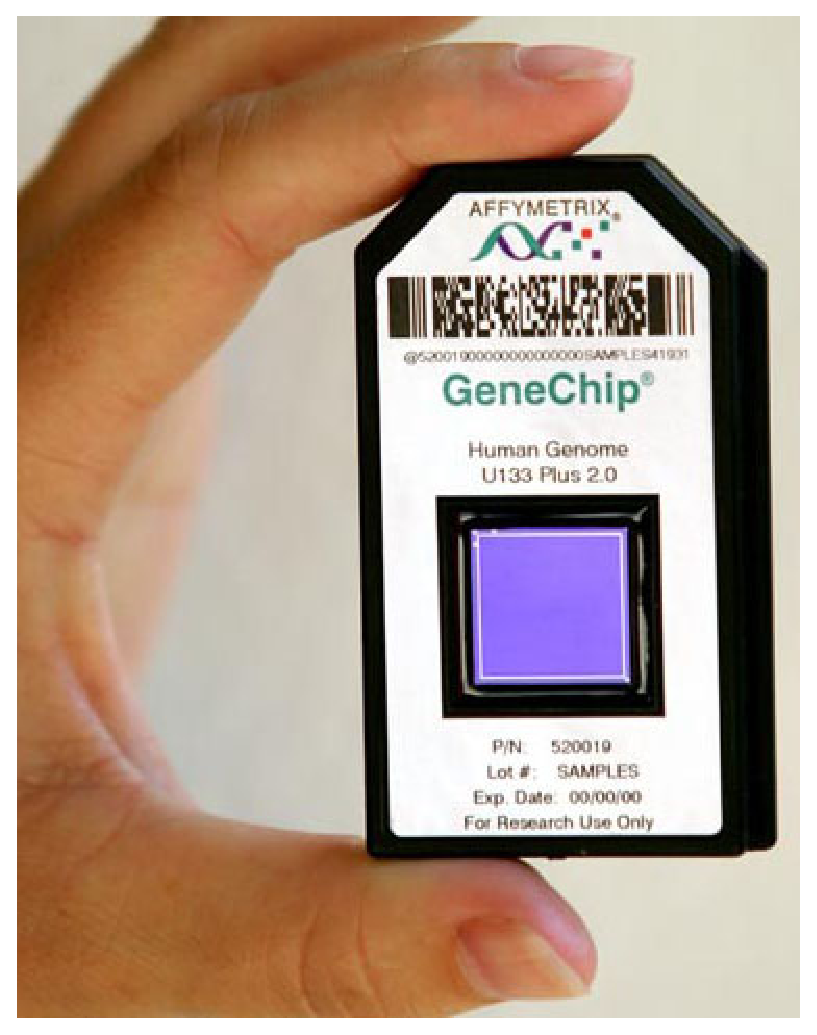
\includegraphics[width=.38\textwidth]{genechip.eps}
\hfill
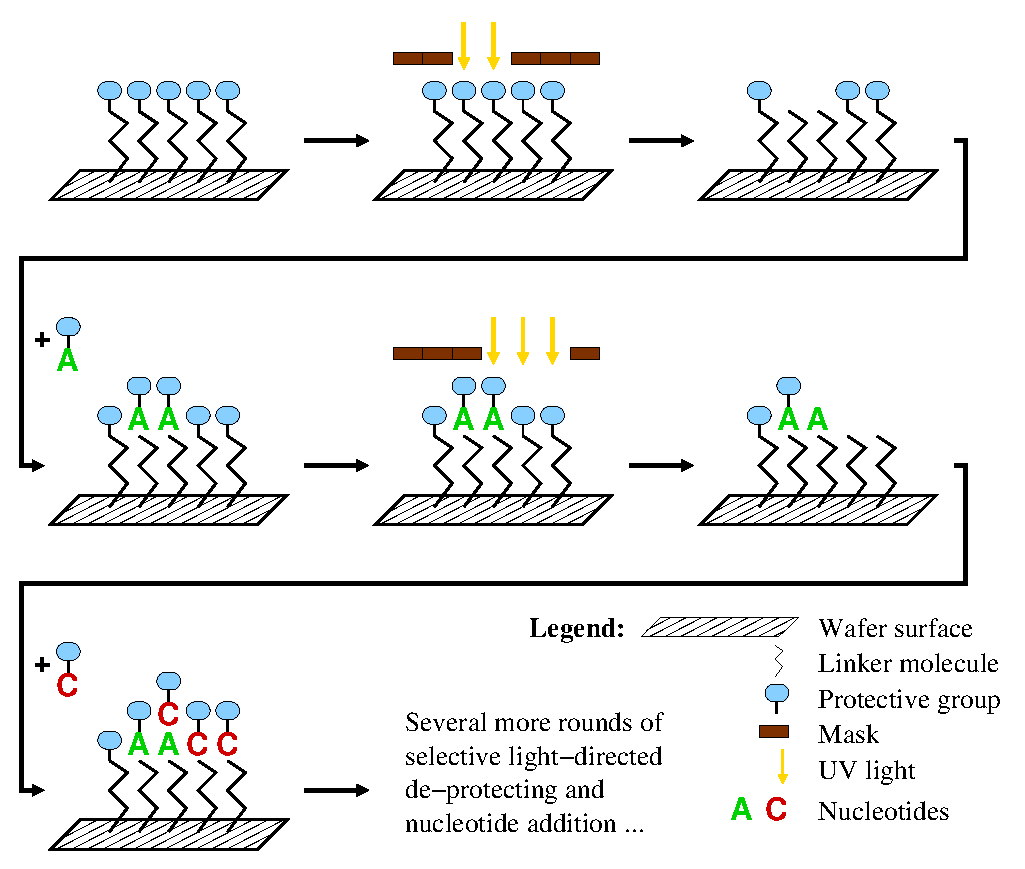
\includegraphics[width=.58\textwidth]{production.eps}
\caption{Left: Affymetrix GeneChip array (source: Affymetrix, Inc.). Right:
probe synthesis via photolithographic masks. The chip is coated with a chemical
compound and a light-sensitive protecting group; masks are used to direct light
and activate selected probes for chemical coupling; nucleotides are appended to
deprotected probes; the process is repeated until all probes have been fully
synthesized.}
\label{fig:photolithography}
\end{figure}

Figure~\ref{fig:photolithography} illustrates this process: The quartz wafer of
a GeneChip array is initially coated with a chemical compound topped with a
light-sensitive protecting group that is removed when exposed to ultraviolet
light, activating the compound for chemical coupling. A lithographic mask is
used to direct light and remove the protecting groups of only those positions
that should receive the nucleotide of a particular synthesis step.  A solution
containing adenine (\tA), thymine (\tT), cytosine (\tC) or guanine (\tG) is then
flushed over the chip surface, but the chemical coupling occurs only in those
positions that have been previously deprotected. Each coupled nucleotide also
bears another protecting group so that the process can be repeated until all
probes have been fully synthesized.

Photolithographic masks are notoriously expensive and cannot be changed once
they have been manufactured. Thus, any change in the chip layout requires the
production of a new set of masks. A similar method of \emph{in situ} synthesis
known as Maskless Array Synthesizer (MAS) was later developed to eliminate the
need of such masks \citep{Singh-Gasson1999}. Probes are still built by repeating
cycles of deprotection and chemical coupling of nucleotides. The illumination,
however, relies on an array of miniature mirrors that can be independently
controlled to direct or deflect the incidence of light on the chip.

NimbleGen Systems, Inc.\ currently uses its Maskless Array Synthesizer (MAS)
technology based on its own Digital Micromirror Device (DMD) similar to Texas
Instruments' Digital Light Processor (DLP) that can control 786\,000 to $4.2$
million individual pixels of light to produce microarrays with spots as small as
16 $\mu$m $\times$ 16 $\mu$m \citep{Nuwaysir2002}. The {\sffamily geniom}\textR\
system of febit biotech GmbH, a highly-automated self-contained platform for
customized microarray production, also uses a micromirror array to direct the
synthesis process \citep{Baum2003}. Recently, the same technology has also been
used to synthesize arrays of peptides using 20 natural amino acids as well as
synthetic amino acid analogs \citep{Pellois2002,Gao2003,Li2004,Bhushan2006}.

\subsection{The unintended illumination problem}

Regardless of which method is used to direct light (masks or micromirror
arrays), it is possible that some probes are accidentally activated for chemical
coupling because of light diffraction, scattering or internal reflection on the
chip surface. This unwanted illumination of regions introduces unexpected
nucleotides that change probe sequences, significantly reducing their chances of
successful hybridization with their targets. Moreover, these faulty probes may
also introduce cross-hybridizations, which can interfere in the experiments
performed with the chip.

This problem is more likely to occur near the borders between a masked and an
unmasked spot (in the case of maskless synthesis, between a spot that is
receiving light and a spot that is not). This observation has given rise to the
term \emph{border conflict}.

It turns out that by carefully designing the \emph{arrangement} of the probes on
the chip and their \emph{embeddings} (the sequences of masked and unmasked steps
used to synthesize each probe), it is possible to reduce the risk of unintended
illumination. This issue becomes even more important as there is a need to
accommodate more probes on a single chip, which requires the production of spots
at higher densities and, consequently, with reduced distances between probes.

%%%%%%%%%%%%%%%%%%%%%%%%%%%%%%%%%%%%%%%%%%%%%%%%%%%%%%%%%%%%%%%%%%%%%%%%%%%%%%%%
\section{Manufacturing and design problems}
\label{sec:intro_problems}

The main focus of this thesis is to design the layout of a microarray in such a
way that we minimize the incidence of the unintended illumination problem, what
we call the \emph{microarray layout problem} (MLP). The MLP is the focus of
Chapters \ref{ch:mlp} to \ref{ch:affy}. A related problem is the \emph{shortest
deposition sequence problem}, which attempts to find the shortest deposition
sequence to synthesize a given set of probes in order to reduce manufacturing
time, cost and probability of errors. This problem is studied in more details in
Chapter \ref{ch:scs}.

We conclude this chapter by briefly describing other interesting mathematical
and computational problems that arise in the design and production of
oligonucleotide microarrays. Recently, \citet{Kahng2003b,Kahng2006} and
\citet{Atlas2004} proposed methodologies to integrate the various steps in the
design of a microarray chip, including probe selection, deposition sequence
design and, ultimely, layout design.

\paragraph{Probe selection.} Although a probe should only hybridize to its
target, it is known that, in practice, cross-hybridizations are likely to occur.
The goal of the probe selection problem is to find the smallest number of probes
with the specified length covering all gene of interest satisfying the three
criteria: homogeneity, sensitivity and specificity as proposed by
\citep{Lockhart1996}. Homogeneity ensures that can hybridize to their targets at
about the same experimental temperature. Sensitivity detects
self-complementarity and prevents probes with secondary structures. Specificity
ensures that probes are unique to each gene and eliminates probes that could
cross-hybridize.

This problem has been extensively studied in the past few years
\citep{Li2001,Kaderali2002}, and many algorithms have been proposed to speed up
the specificity check, regarded as the most computational intensive step
\citep{Rahmann2002,Sung2003,Chou2004}. Among the presented approaches,
\cite{Rahmann2002} proposed a fast algorithm based on suffix arrays
\citep{Manber1990} that eliminates candidates that have a long common factor
with other genes.

\paragraph{Mask decomposition problem.} Once the probes have been selected and
the layout of the chip has been designed, the photolithographic masks must be
produced. The masks used by Affymetrix are fabricated by a series of
``flashes'', with each flash producing a rectangular part of the mask. The cost
of a mask is directly proportional to the number of flashes
\citep{Hubbell1998,Hubbell1999} and, in fact, there may be a limit in the number
of flashes before a more expensive fabrication technology must be used. Ideally,
each mask must be decomposed in the minimum number of rectangles in order to
reduce costs and incidence of errors.

\citet{Hannenhalli2002} studied this problem, called the mask decomposition
problem, as an instance of the rectilinear polygon interior cover problem,
which, according to \citet{Garey1979} was first shown to be NP-hard by
\citet{Masek}. Although approximation algorithms with small performance ratios
are known \citep{Franzblau1986}, \citet{Hannenhalli2002} explored the particular
characteristics of photolithographic masks to devise an efficient algorithm
which found provably optimal decompositions for a set of relatively small
GeneChip arrays.

\paragraph{Probe quality control.} During the production of a microarray chip,
it is possible that one synthesis step may be entirely compromised, resulting in
damages to all probes that receive the nucleotide of that particular step, and,
consequently, invalidating any experimental result obtained with the chip. In
order to detect such failures, Affymetrix have introduced the idea of producing a
set of \emph{quality control probes} (QC) on their chips \citep{Affymetrix2002}.
Target molecules for each QC probe are deliberately added to the biological
mixture during the experiment with the chip. If no synthesis step fails, the QC
probes should exhibit similar signal intensities. Thus, by measuring the
fluorescent signal emitted by each QC probe, it is possible to infer if they
have been correctly synthesized or not.

In fact, several copies of each quality control probe are produced on different
spots of the chip using different synthesis schedules (embeddings) in such a way
that it is possible to check if a synthesis step was compromised
\citep{Hubbell1999a} (and maybe even identify systematic problems in the chip
production). However, the validation proposed by \citet{Hubbell1999a} does not
take into account possible defects on isolated spots containing QC probes caused
by other manufacturing problems. For this reason, robust schemes based on a
combinatorial design approach that guarantee coverage of all synthesis steps and
that are able to tolerate a great number of unreliable QC probes have been
proposed \citep{Alon2001,Sengupta2002,Colbourn2002,Khan2003}.

%%%%%%%%%%%%%%%%%%%%%%%%%%%%%%%%%%%%%%%%%%%%%%%%%%%%%%%%%%%%%%%%%%%%%%%%%%%%%%%%
\chapter{The Microarray Layout Problem}
\label{ch:mlp}
%%%%%%%%%%%%%%%%%%%%%%%%%%%%%%%%%%%%%%%%%%%%%%%%%%%%%%%%%%%%%%%%%%%%%%%%%%%%%%%%

In this chapter we give a more precise definition of the Microarray Layout
Problem (MLP) and define criteria for evaluating a given layout. The description
that follows assumes that probes are synthesized with photolithographic masks,
but the concepts also apply to the maskless production (with micromirror
arrays). Two evaluation criteria are presented: \emph{border length} and
\emph{conflict index}. As shown later, the conflict index model can be seen as a
generalization of the border length model.

Formally, we have a set of probes $\CalP = \{p_{1}, p_{2}, \dots, p_{n}\}$,
where each $p_k \in \{\text{A,C,G,T}\}^\ast$ with $1 \leq k \leq n$ is produced
by a series of $T$
synthesis steps. Frequently, but not necessarily, all probes have the same
length $\ell$. Each synthesis step $t$ uses a mask $M_t$ to induce the addition
of a particular nucleotide $N_t \in \{\text{A,C,G,T}\}$ to a subset of~$\CalP$
(Figure~\ref{fig:masking_process}). The \emph{nucleotide deposition sequence}
$N = N_{1} N_{2} \ldots N_{T}$ corresponding to the sequence of nucleotides
added at each synthesis step is a supersequence of all $p \in \CalP$.

A microarray chip consists of a set of spots, or sites,
$\CalS = \{s_{1}, s_{2}, \dots, s_{m}\}$, where each spot $s$ is specified by
its coordinates on the chip surface and accommodates a unique probe
$p_k \in \CalP$. Note that we usually refer to $s$ as containing a single probe
$p_k$ although, in practice, it contains several million copies of it. Each
probe is synthesized at a unique spot, hence there is a one-to-one assignment
between probes and spots (if we assume that there are as many spots as probes,
i.e., $m=n$). Real microarrays may have complex physical structures but
we assume that the spots are arranged in a rectangular grid with
$n_r$ rows and $n_c$ columns. We also assume that probes can be assigned to any
spot.

In general, a probe can be \emph{embedded} within $N$ in several ways. An
embedding of $p_{k}$ is a $T$-tuple
$\eps_{k} = (\eps_{k,1}, \eps_{k,2}, \dots, \eps_{k,T})$ in which
$\eps_{k,t} = 1$ if probe $p_{k}$ receives nucleotide $N_{t}$ (at step~$t$), and
0 otherwise. In particular, a \emph{left-most embedding} is an embedding in
which the bases are added as early as possible (as in $\eps_1$ in
Figure~\ref{fig:masking_process}). Similarly, a \emph{right-most embedding} is
an embedding in which the bases are added as late as possible (as in $\eps_8$ in
Figure~\ref{fig:masking_process}).

We say that an embedding $\eps_k$ is \emph{productive} (unmasked) at step $t$ if
$\eps_{k,t} = 1$, or \emph{unproductive} (masked) otherwise. The terms
productive and unproductive can also be used to denote unmasked and masked
spots, respectively.

\begin{figure}[t]\centering
\centerline{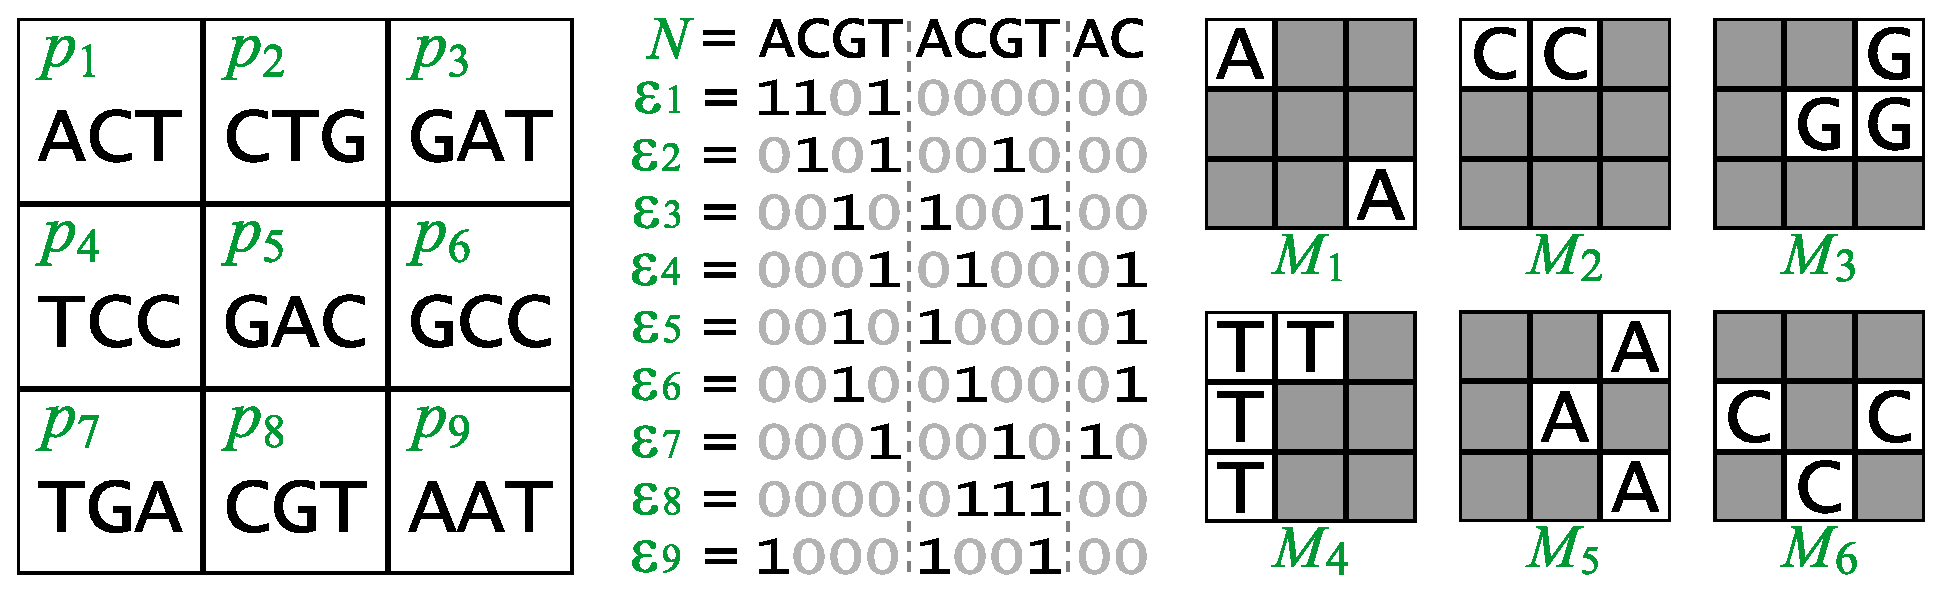
\includegraphics[width=\textwidth]{figures/chip.eps}}
\caption{Synthesis of a hypothetical 3$\times$3 chip with photolithographic
  masks. Left: chip layout and the 3-mer probe sequences. Center: deposition
  sequence with 2.5 cycles (cycles are delimited with dashed lines) and probe
  embeddings (asynchronous). Right: first six masks (masks 7 to 10 not shown).}
\label{fig:masking_process}
\end{figure}

The deposition sequence is often a repeated permutation of the alphabet, mainly
because of its regular structure and because such sequences maximize the number
of distinct subsequences \citep{Chase1976}. The deposition sequence shown in
Figure~\ref{fig:masking_process} is a 2.5-time repetition of ACGT, and we thus
say that it has two and a half \emph{cycles}.

For cyclic deposition sequences, it is possible to distinguish between two types
of embeddings: \emph{synchronous} and \emph{asynchronous}. In the former, each
probe has exactly one nucleotide synthesized in every cycle of the deposition
sequence; hence, 25 cycles or 100 steps are needed to synthesize probes of
length 25. In the latter, probes can have any number of nucleotides synthesized
in any given cycle, allowing shorter deposition sequences. For this reason,
asynchronous embeddings are usually the choice for commercial microarrays.  For
instance, all GeneChip arrays that we know of can be asynchronously synthesized
in 74~steps with 18.5 cycles of TGCA --- we refer to this sequence as the
\emph{standard Affymetrix deposition sequence} (see Chapter~\ref{ch:affy}).

Ideally, the deposition sequence should be as short as possible in order to
reduce manufacturing time, cost and probability of errors \citep{Rahmann2003}.
Finding the shortest deposition sequence to synthesize a set of probes is an
instance of a classical computer science problem known as the Shortest Common
Supersequence problem, which will be the focus of Chapter~\ref{ch:scs}. For the
MLP, however, we assume that $N$ is a fixed sequence given as input.

%%%%%%%%%%%%%%%%%%%%%%%%%%%%%%%%%%%%%%%%%%%%%%%%%%%%%%%%%%%%%%%%%%%%%%%%%%%%%%%%
\section{Problem statement}
\label{sec:mlp_problem}

Given a set of probes $\CalP$, a geometry of spots $\CalS$, and a deposition
sequence $N$ as specified above, the MLP asks to specify a chip layout
$(\lambda,\eps)$ that consists of
\begin{enumerate}
\item a bijective assignment $\lambda: \CalS\to \{1,\dots,n\}$ that specifies a
  probe index $k(s)$ for each spot $s$ (meaning that $p_{k(s)}$ will be
  synthesized at $s$),
\item an assignment $\eps: \{1,\dots,n\}\to \{0,1\}^T$ specifying an embedding
  $\eps_k = (\eps_{k,1},\dots,\eps_{k,T})$ for each probe index $k$, such that
  $N[\eps_k] :\equiv (N_t)_{t: \eps_{k,t}=1} = p_k$,
\end{enumerate}
such that a given penalty function is minimized.  We introduce two such penalty
functions: total border length and total conflict index.

%We may thus speak of $\eps_{k(s)}$ as the embedding at spot $s$.

%%%%%%%%%%%%%%%%%%%%%%%%%%%%%%%%%%%%%%%%%%%%%%%%%%%%%%%%%%%%%%%%%%%%%%%%%%%%%%%%
\section{Border length}
\label{sec:mlp_border_length}

The first formal definition of the unintended illumination problem was given by
\citet{Hannenhalli2002}, who defined the \emph{border length}~$\CalB_t$ of a
mask~$M_{t}$ as the number of borders separating masked and unmasked spots at
synthesis step~$t$, that is, the number of border conflicts in $M_{t}$.
Formally,
%%
\begin{equation}
\label{eq:border_length}
  \CalB_t := \frac{1}{2} \cdot \sum_{s,s' \in \CalS}
    \Ind{s \text{ and } s' \text{ are adjacent}}
    \cdot \Ind{\eps_{k(s),t} \neq \eps_{k(s'),t}}.
\end{equation}
%%
where $\Ind{cond}$ is the indicator function that equals 1 if condition $cond$
is true, and 0 otherwise. The \emph{total border length} of a given layout
$(\lambda,\eps)$ is the sum of border lengths over all masks, that is
%%
\begin{equation}
\label{eq:total_border_length}
  \CalB(\lambda,\eps) := \sum_{t=1}^{T} \CalB_t.
\end{equation}

The \emph{Border Length Minimization Problem} was then defined as the problem of
finding a layout minimizing the total border length \citep{Hannenhalli2002}. As
an example, the six masks shown in Figure~\ref{fig:masking_process} have
$\CalB_1 = 4$, $\CalB_2 = 3$, $\CalB_3 = 5$, $\CalB_4 = 4$, $\CalB_5 = 8$ and
$\CalB_6 = 9$. The total border length of that layout is 52 (masks $M_7$ to
$M_{10}$ are not shown).

\paragraph{Hamming distance.}
In the next chapters, we refer to the \emph{Hamming distance} $H(k,k')$ between
the embeddings $\eps_k$ and $\eps_{k'}$ as the number of synthesis steps in
which they differ. Formally,
%%
\begin{equation}\label{eq:hamming}
  H(k,k') := \sum_{t=1}^{T} \Ind{\eps_{k,t} \neq \eps_{k',t}}.
\end{equation}

Note that $H(k,k')$ gives the number of border conflicts generated when probes
with embeddings $\eps_k$ and $\eps_{k'}$ are placed in adjacent spots.

\subsection{Lower bounds}

Lower bounds for the BLMP with synchronous and asynchronous embeddings were
given by \citet{Kahng2002}, based on a simple graph formulation. Unfortunately,
both lower bounds are not tight, and their computation is time-consuming,
especially for large chips.

\paragraph{Synchronous embeddings.}
Let $L$ be a complete directed graph over the set of probes $\CalP$ with arcs
weighted with the Hamming distance between the (unique) embeddings of the
corresponding probes.

Since a probe can have at most four neighbors on the chip, we delete all but the
four arcs with the least weights of every node. Furthermore, assuming that the
chip is a rectangular grid with $n_r$ rows and $n_c$ columns, we delete the
heaviest $2 \cdot (n_r + n_c)$ remaining arcs, because the spots on the borders
of the chip have less than four neighbors. It is not difficult to see that the
cost of any placement must be greather than the total arc weight of $L$, and we
obtain the following theorem.

\begin{theorem}
  \label{thm:sync_lb}
  The total arc weight of $L$ is a lower bound on the total border length of
  the optimum layout with synchronous embeddings.
\end{theorem}

\paragraph{Asynchronous embeddings.}
With asynchronous embeddings, we can construct a similar complete directed graph
$L'$. For the arc weights, however, it is necessary to estimate the minimum
number of border conflicts between the two probes (among all of their possible
embeddings).

\citet{Kahng2002} observed that the number of bases of a probe $p_k$ that can
be ``aligned'' with bases of $p_{k'}$ cannot exceed the length of $LCS(p_k,p_{k'})$,
where $LCS(p_k,p_{k'})$ is the
\emph{longest common subsequence} of $p_k$ and $p_{k'}$. Therefore, an arc of $L'$
between probes $p_k$ and $p_{k'}$ can be weighted with $\ell - |LCS(p_k,p_{k'})|$,
where $\ell$ is the length of both probe sequences (assuming probes have the same length).

We can then delete all but the four arcs with the least weights of each probe
and, subsequently, the heaviest $2 \cdot (n_r + n_c)$ remaining arcs of $L'$, to
obtain the following theorem.

\begin{theorem}
  \label{thm:async_lb}
  The total arc weight of $L'$ is a lower bound on the total border length of
  the optimum layout with asynchronous embeddings.
\end{theorem}

%%%%%%%%%%%%%%%%%%%%%%%%%%%%%%%%%%%%%%%%%%%%%%%%%%%%%%%%%%%%%%%%%%%%%%%%%%%%%%%%
\section{Conflict index}
\label{sec:mlp_conflict_index}

The border length measures the quality of an individual mask or set of masks.
With this model, however, it is not possible to know how the border conflicts
are distributed among the probes. Ideally, all probes should have roughly the
same risk of being damaged by unintended illumination, so that all signals are
affected in approximately the same way.

The \emph{conflict index} is a quality measure defined with the aim of
estimating the risk of damaging probes at a particular spot
\citep{Carvalho2006a}; it is thus a per-spot or per-probe measure instead of a
per-mask measure. Additionally, it takes into account two practical
considerations observed by \citet{Kahng2003}:
%%
\begin{itemize}
\item[a)] stray light might activate not only adjacent neighbors but also spots
  that lie as far as three cells away from the targeted spot;
\item[b)] imperfections produced in the middle of a probe are more harmful than
  in its extremities.
\end{itemize}

For a proposed layout $(k,\eps)$, the conflict index~$\CalC(s)$ of a spot $s$
whose probe $p_{k(s)}$ is synthesized in $T$~masking steps according to its
embedding vector $\eps_{k(s)}$ is
%%
\begin{equation}
\label{eq:conf_idx}
\CalC(s) := \sum_{t=1}^{T} \Bigl(
  \Ind{\eps_{k(s),t}=0}
  \cdot \omega(\eps_{k(s)},t)
  \cdot \sum_{\substack{s'\text{: neighbor}\\\text{of } s}}
  \Ind{\eps_{k(s'),t}=1}
  \cdot \gamma(s,s') \Bigr).
\end{equation}

The indicator functions ensure the following conflict condition: During
step~$t$, there is a conflict at spot~$s$ if and only if $s$ is masked
($\eps_{k(s),t}=0$) and a close neighbor $s'$ is unmasked ($\eps_{k(s'),t}=1$)
--- since light directed at $s'$ may somehow reach $s$. When $s$ is unmasked, it
does not matter if it accidentally receives light targeted at a neighbor, and
when $s'$ is masked, there is no risk that it damages probes of $s$ since it is
not receiving light.

\begin{figure}[t]\centering
%%
\begin{picture}(435,150)
  \put(0,0){\makebox(180,150){
    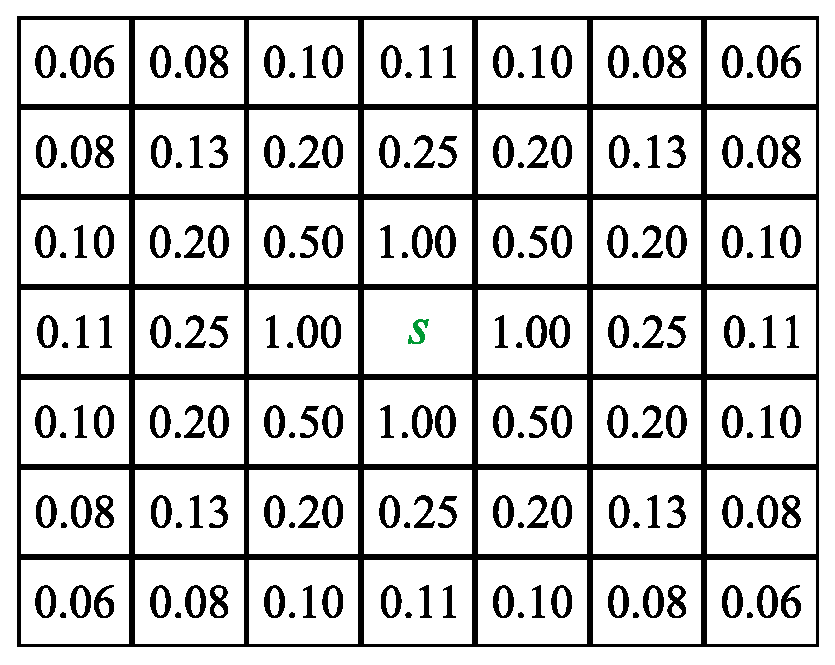
\includegraphics[width=0.4\textwidth]{distweights}
  }}
  \put(180,5){\makebox(255,145){
    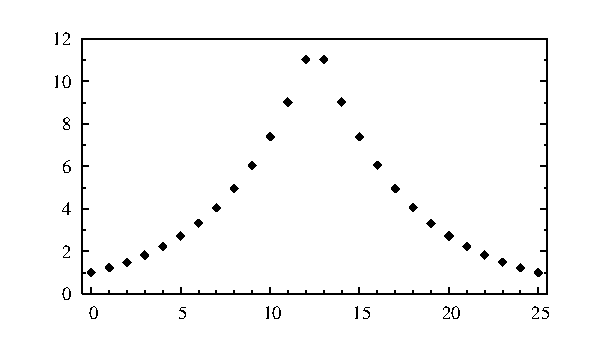
\includegraphics{posweights}
  }}
\end{picture}
%%
\vspace*{-3ex}
\caption{\label{fig:conflictindex}
  Ranges of values for both $\gamma$ and $\omega$ on a typical Affymetrix chip
  where probes of length $\ell=25$ are synthesized in $T=74$ masking steps.
  Left: approximate values of the distance-dependent weighting function
  $\gamma(s,s')$ for a spot $s$ in the center and close neighbors~$s'$. Right:
  position-dependent weights $\omega(\eps,t)$ on the y-axis for each value of~
  $b_{\eps,t}\in\{0,\dots,25\}$ on the x-axis, using $\theta = 5/\ell$ and
  $c = 1/\exp{(\theta)}$.
  }%
\end{figure}

Function $\gamma(s,s')$ is a ``closeness'' measure between $s$ and $s'$ (to
account for observation a). We defined it as
%%
\begin{equation}\label{eq:dist_weight}
\gamma(s,s') := (d(s,s'))^{-2},\nopagebreak
\end{equation}\nopagebreak
%%
where $d(s,s')$ is the Euclidean distance between the spots $s$ and $s'$. Note
that in (\ref{eq:conf_idx}), $s'$ ranges over all neighboring spots that are at
most three cells away from $s$ (see Figure~\ref{fig:conflictindex}, left), which
is in accordance with observation a.

In general, we use the terms \emph{close neighbor} or simply \emph{neighbor} of
a spot $s$ to refer to a spot $s'$ that is at most three cells away (vertically
and horizontally) from $s$. In other words, $s'$ is inside a $7\times 7$ region
centered around $s$. This is in contrast to the terms \emph{direct} or \emph{
immediate neighbor} of $s$, used to denote a spot $s'$ that is adjacent to $s$
(in other words, when $s'$ shares a common border with $s$ on the chip).
Obviously, an immediate neighbor $s'$ is also a close neighbor of $s$.

The position-dependent weighting function $\omega(\eps,t)$ accounts for the
significance of the location inside the probe where the undesired nucleotide is
introduced in case of accidental illumination (observation b). We defined it as:
%%
\begin{equation}\label{eq:pos_mult}
\omega(\eps,t) := c \cdot \exp{\left(\theta \cdot \lambda(\eps,t)\right)}
\end{equation}
%%
where $c>0$ and $\theta>0$ are constants, and for $1\leq t\leq T$,
%%
\begin{equation}\label{eq:base_pos}
  \lambda(\eps,t) := 1 + \min(b_{\eps,t},\ell_{\eps} - b_{\eps,t}),
\end{equation}
%%
\begin{equation}\label{eq:b_ell}
  b_{\eps,t} := \sum_{t'=1}^{t} \eps_{t'},
  \qquad
  \ell_{\eps} := \sum_{t=1}^{T} \eps_t = b_{\eps,T}.
\end{equation}

In other words, $\ell_\eps$ is the length of the final probe specified by $\eps$
(equal to the number of ones in the embedding), and $b_{\eps,t}$ denotes the
number of nucleotides synthesized up to and including step~$t$.

We can now speak of the \emph{total conflict index} of a given layout
$(\lambda,\eps)$ as the sum of conflict indices over all spots, that is
%%
\begin{equation}
\label{eq:total_conf_idx}
  \CalC(\lambda,\eps) := \sum_{s} \CalC(s).
\end{equation}

\paragraph{Conflict index distance.}
Many of the algorithms discussed in later chapters were initially developed for
border length minimization, and they usually rely on the Hamming distance
defined earlier (\ref{eq:hamming}). We have adapted some of these algorithms to
work with conflict index minimization by using the \emph{conflict index
distance}, which extends the Hamming distance by taking into account the
position inside the probe where the conflict occurs (observation b). The
conflict index distance $C(k,k')$ between the embeddings $\eps_k$ and
$\eps_{k'}$ is defined as:
%%
\begin{equation}
\label{eq:ci_dist}
C(k,k') := \sum_{t=1}^{T}
  \Bigl(
    \Ind{\eps_{k,t}=0 \text{ and } \eps_{k',t}=1}
    \cdot \omega(\eps_{k},t)
    +
    \Ind{\eps_{k',t}=0 \text{ and } \eps_{k,t}=1}
    \cdot \omega(\eps_{k'},t)
  \Bigr).
\end{equation}

The conflict index distance $C(k,k')$ can be interpreted as the sum of the
conflict indices resulting from placing probes with embeddings $\eps_k$ and
$\eps_{k'}$ at hypothetical neighboring spots, ignoring the distance between
these spots (note that there is no dependency on $\gamma$) and the conflicts
generated by other neighbors.

\subsection{The choices of $\gamma$ and $\omega$}

The conflict index $\CalC(s)$ attempts to estimate the risk of damaging the
probes of a spot $s$ due to unintended illumination. The definitions of $\gamma$
and $\omega$ given here are an arbitrary choice in an attempt to capture the
characteristics of the problem.

However, the most appropriate choice of $\gamma$ depend on several attributes of
the specific technology utilized to produce the chips such as the size of the
spots, the density of the probes on the chip, the physical properties of the
light being used (intensity, frequency, etc.), the distance between the light
source and the mask, and the distance between the mask (or the micromirrors) and
the chip surface.

The most appropriate choice of $\omega$ depend on the chemical properties of the
hybridization between probes and targets. Although it is generally agreed that
the chances of a successful hybridization are higher if a mismatched base occurs
at the extremities of the formed duplex instead of at its center
\citep{Hubbell1999}, the precise effects of this position is not yet fully
understood and has been an active topic of research \citep{Binder2005}.

We propose the use of an exponential function, so that $\omega$ grows
exponentially from the extremities of the probe to its center (see
Figure~\ref{fig:conflictindex}, right). The motivation behind this definition is
that the probability of a successful stable hybridization of a probe with its
target should increase exponentially with the absolute value of its Gibbs free
energy, which increases linearly with the length of the longest perfect match
between probe and target.

The parameter $\theta$ controls how steeply the exponential weighting function
rises towards the middle of the probe. In our experiments, unless stated
otherwise, we use probes of length $\ell=25$, and parameters $\theta = 5/\ell$
and $c = 1/\exp{(\theta)}$.

Finding the best choice of $\gamma$ and $\omega$ for a particular technology is
beyond the scope of this thesis. We note, however, that all algorithms discussed
in the next chapters were developed to work independently of the values given by
these functions. In other words, should $\gamma$ and $\omega$ be defined
differently, no changes to the algorithms are necessary.

%%%%%%%%%%%%%%%%%%%%%%%%%%%%%%%%%%%%%%%%%%%%%%%%%%%%%%%%%%%%%%%%%%%%%%%%%%%%%%%%
\section{Chip quality measures}
\label{sec:mlp_bl_vs_ci}

Most of the algorithms discussed in the next chapters can work with border
length as well as conflict index minimization. In our experiments, we will
usually present results with both measures, making a distinction between border
length minimization (BLM) and conflict index minimization (CIM).

The relation between these two
measures becomes clear if $\gamma(s,s')$ and $\omega(\eps,t)$ are re-defined as
follows: Set $\gamma(s,s') := 1$ if $s'$ is a direct neighbor of~ $s$, and $:=0$
otherwise. Also, set $c=1/2$ and $\theta=0$ so that $\omega(\eps,t) := 1/2$
independently of the position in the probe where the conflict occurs. Now
$\sum_s\, \CalC(s) = \sum_{t=1}^T\, \CalB_t$; that is, total border length is
equivalent to the total conflict index for a particular choice of $\gamma$ and
$\omega$. For the choices~(\ref{eq:dist_weight}) and~(\ref{eq:pos_mult}), they
are not equivalent but still correlated, since a good layout has low border
lengths as well as low conflict indices.

To better compare border lengths for chips of different sizes, we usually divide
the total border length by the number $n_b$ of internal borders of the chip,
which equals $n_r(n_c - 1) + n_c(n_r - 1)$ if the the chip is a rectangular grid
with $n_r$ rows and $n_c$ columns. We thus call $\CalB(\lambda,\eps)/n_b$ the
\emph{normalized border length}, NBL for short, of a given layout
$(\lambda,\eps)$. This can be further divided by the number of synthesis steps
to give the \emph{normalized border length per mask}
$\CalB(\lambda,\eps)/(n_b \cdot T)$. We may also refer to the normalized border
length of a particular mask $M_t$ as $B_t/n_b$. Since $B_t \leq n_b$,
$B_t/n_b \leq 1$ and thus $\CalB(\lambda,\eps)/n_b \leq T$.

Similarly, it is useful to divide the total conflict index by the number of
probes on the chip, and we define the \emph{average conflict index}, ACI for
short, of a layout as $\CalC(\lambda,\eps)/|\CalP|$.

%%%%%%%%%%%%%%%%%%%%%%%%%%%%%%%%%%%%%%%%%%%%%%%%%%%%%%%%%%%%%%%%%%%%%%%%%%%%%%%%
\section{How hard is the Microarray Layout Problem?}
\label{sec:mlp_how_hard}

The MLP appears to be hard because of the super-exponential number of possible
arrangements, although no NP-hardness proof is yet known. A formulation of the
MLP as a Quadratic Assignment Problem (QAP) is given in Chapter~\ref{ch:qap}.
The QAP is a classical combinatorial optimization problem that is, in general,
NP-hard, and particularly hard to solve in practice \citep{Cela1997}. Optimal
solutions are thus unlikely to be found even for small chips and even if we
assume that all probes have a single predefined embedding.

If we consider all possible embeddings (up to several million for a typical
Affymetrix probe), the MLP is even harder. For this reason, the problem has been
traditionally tackled in two phases. First, an initial embedding of the probes
is fixed and an arrangement of these embeddings on the chip with minimum
conflicts is sought. This is usually referred to as the \emph{placement} phase.
Second, a post-placement optimization phase \emph{re-embeds} the probes
considering their location on the chip, in such a way that the conflicts with
neighboring spots are further reduced. Often, the chip is \emph{partitioned}
into smaller sub-regions before the placement phase in order to reduce running
times, especially on larger chips.

The most important placement algorithms are surveyed in
Chapter~\ref{ch:placement}, whereas re-embedding algorithms are discussed in
Chapter~\ref{ch:reembed}. Partitioning algorithms are the focus of
Chapter~\ref{ch:part}. Finally, we present recent developments that
simultaneously place and re-embed probes in Chapter~\ref{ch:merge}.

%%%%%%%%%%%%%%%%%%%%%%%%%%%%%%%%%%%%%%%%%%%%%%%%%%%%%%%%%%%%%%%%%%%%%%%%%%%%%%%%
\chapter{Placement Algorithms}
\label{ch:placement}
%%%%%%%%%%%%%%%%%%%%%%%%%%%%%%%%%%%%%%%%%%%%%%%%%%%%%%%%%%%%%%%%%%%%%%%%%%%%%%%%

The input for a placement algorithm consists of the deposition sequence $N$,
a set of probes $\mathcal{P}$ (each probe is assumed to have at least one
embedding in $N$) and a geometry of spots $\mathcal{S}$. In practice,
microarrays may have complex physical structures but we assume that the spots
are arranged in a rectangular grid with $n_r$ rows and $n_c$ columns. We also
assume that probes can be assigned to any spot.

The output of a placement algorithm is a one-to-one assignment of probes to
spots. If there are more spots than probes to place, we can add enough ``empty''
probes that do not introduce any conflicts with the other probes (since light
is never directed to such spots).

All algorithms discussed in this section assume that an initial embedding
of the probes is given, which can be a left-most, right-most, synchronous or
otherwise pre-computed embedding --- a placement algorithm typically does not
change the given embeddings.


\section{Early approaches}
\label{sec:placement_early}

\begin{figure}
\begin{picture}(330,100)
\put(0,0){\makebox(110,15){a)}}
\put(110,0){\makebox(110,15){b)}}
\put(220,0){\makebox(110,15){c)}}
\put(-3,15){  \makebox(110,85){\includegraphics[width=0.3\textwidth]{0threading}}}
\put(110,15){\makebox(110,85){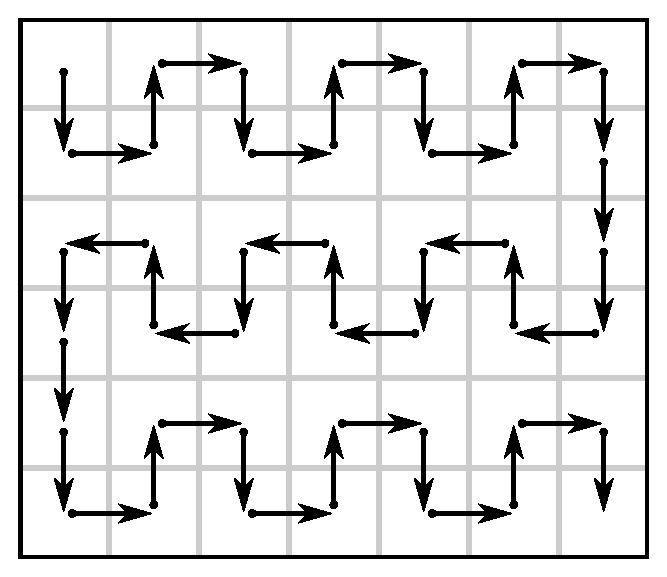
\includegraphics[width=0.3\textwidth]{1threading}}}
\put(220,15){\makebox(110,85){\includegraphics[width=0.3\textwidth]{2threading}}}
\end{picture}
\caption{\label{fig:threading}%
  Different ways of \emph{threading} probes on a chip. a) Standard
  row-by-row (0-threading); b) 1-threading; c) 2-threading.}%
\end{figure}

\citet{Feldman1994} were the first to formally address the unintended
illumination problem. They showed how an optimal placement can be constructed
based on a two-dimensional Gray code.  Their work, however, is restricted to
\emph{uniform arrays} (arrays containing all $4^\ell$ probes of a given length
$\ell$) and synchronous embeddings, being thus of limited practical importance
for current microarrays.

The border length problem on arrays of arbitrary probes was first
discussed by \citet{Hannenhalli2002}. The article reports that the
first Affymetrix chips were designed using a heuristic for the
traveling salesman problem (TSP). The idea is to build a weighted
graph with nodes representing probes, and edges containing the Hamming
distances between their embeddings, that is, the number of times their
embeddings differ at a particular synthesis step. A TSP tour on this
graph is heuristically constructed, resulting in consecutive probes in
the tour being likely similar. The TSP tour is then \emph{threaded} on
the array in a row-by-row fashion (Fig.~\ref{fig:threading}a).

Hannenhalli and co-workers studied several threading alternatives,
which they collectively called \emph{$k$-threading}
(Fig.~\ref{fig:threading}b,c). A $k$-threading is a variation of the
standard row-by-row threading, in which the right-to-left and
left-to-right paths are interspaced with alternating upward and
downward movements over $k$ sites. (The row-by-row threading can be
seen as a $k$-threading with $k=0$.) Hannenhalli and co-workers
experimentally observed that 1-threading may reduce border length in up to
20\% for large chips when compared to row-by-row threading.

A different strategy, called Epitaxial placement, was proposed by
\citet{Kahng2002}. It was originally designed for chips with synchronous
embeddings, but it can be trivially implemented for asynchronous embeddings as
well. The algorithm starts by placing a random probe in the center of the array
and continues to insert probes in spots adjacent to already-filled spots.
Priority is given to spots whose all four neighbors are full, in which case a
probe with the minimum number of border conflicts with the neighbors is placed.
Otherwise, all spots~$s$ with $i \geq 1$ filled neighbors are examined. For each
spot, the algorithm finds a non-assigned probe~$p$ whose number of conflicts
with the filled neighbors, $c(s,p)$, is minimal, and assigns a cost
$C(s,p) = k_i \cdot c(s,p) / i$ for this assignment, where $0 < k_i \leq 1$ are
scaling coefficients (the authors propose $k_1 = 1$, $k_2 = 0.8$, and
$k_3 = 0.6$). The assignment with minimum $C(s,p)$ is made and the procedure is
repeated until all probes have been placed. With this algorithm, Kahng and
co-workers claim a further 10\% reduction in border conflicts over
TSP\,+\,1-threading.

Both the Epitaxial algorithm and the TSP approach have at least quadratic time
complexity and hence do not scale well to large chips. This observation
motivated the design of two new placement algorithms: Sliding-Window Matching
(SWM) and Row-Epitaxial \citep{Kahng2003}.



\section{Sliding-Window Matching}
\label{sec:placement_swm}

\begin{figure}[t!]
\centerline{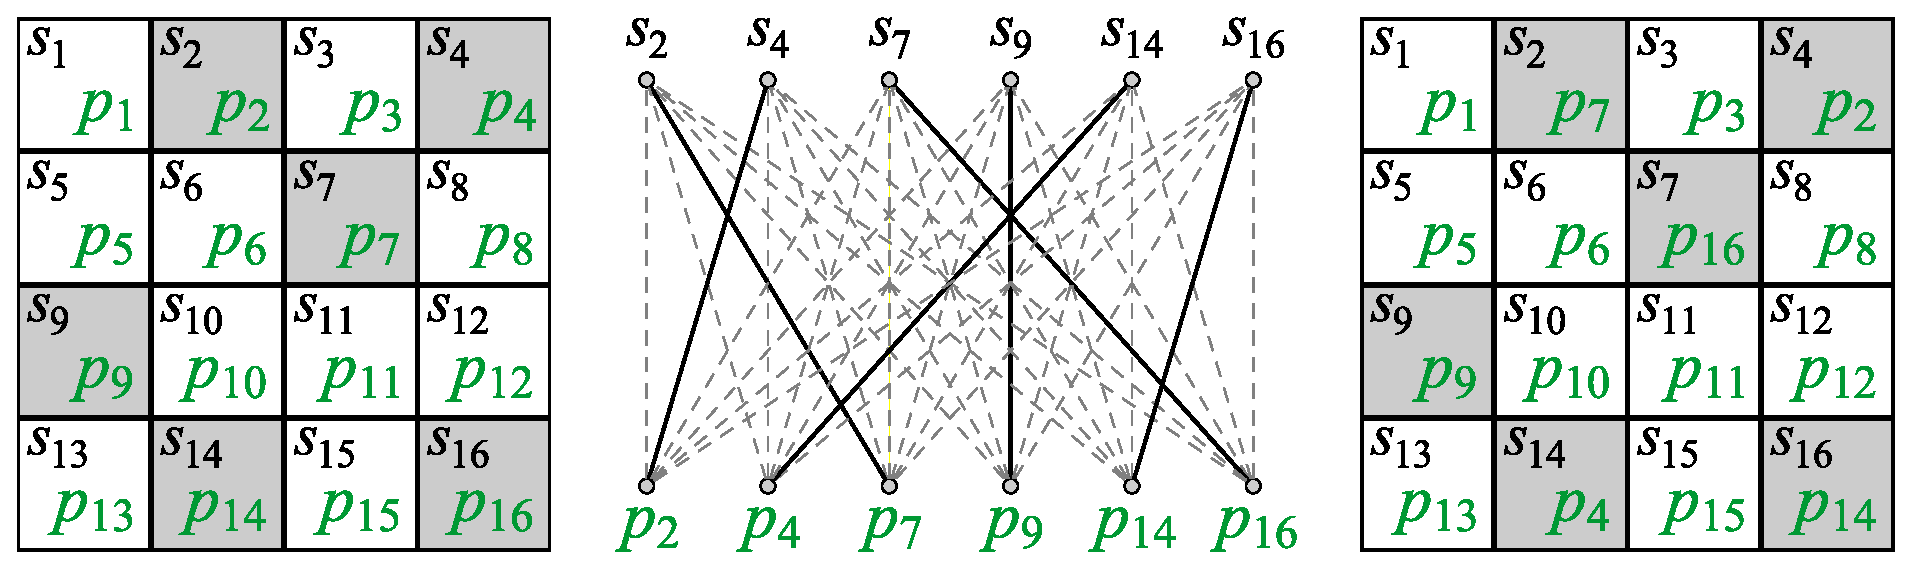
\includegraphics[width=\textwidth]{swm.eps}}
\begin{picture}(340,15)
\put(0,0){\makebox(95,15){a)}}
\put(95,0){\makebox(145,15){b)}}
\put(240,0){\makebox(95,15){c)}}
\end{picture}
\caption{\label{fig:swm}%
  Sliding-Window Matching algorithm. a) Initial arrangement of probes
  $p_1 \dots p_{16}$ inside a $4 \times 4$ window and the selected independent
  set of spots (shaded). b) Bipartite graph and a minimum weight perfect
  matching (dark edges). c) New arrangement inside the window.}%
\end{figure}

The SWM is not exactly a placement algorithm as it iteratively improves an
existing placement that can be constructed, for instance, by
TSP\,+\,1-threading, or much simpler, by lexicographically sorting the binary
embedding vectors with a linear-time radix sort. The sorting is several times
faster but it is also likely to produce a worse initial placement than the
TSP, with consecutive embeddings being similar only in their first synthesis
steps. This, however, should be of little importance given that this placement
is only used as a starting point for the SWM algorithm.

The SWM works inside a window that starts at the top left of the chip
and slides from left to right, top to bottom, while maintaining a
certain amount of overlap between each iteration. When the window
reaches the right-end of the chip, it is re-started at the left-end of
the next set of rows, also retaining an overlap with the preceding
rows.

At each iteration, the algorithm attempts to reduce the total border
length inside the window by relocating some probes
(Fig.~\ref{fig:swm}a).  First, a random maximal independent set
of spots is selected, and the probes assigned to these spots are
removed. The term independent refers to the fact that selected spots
can be re-assigned to probes without affecting the border length of
other selected spots. The algorithm creates a bipartite graph with
nodes representing the removed probes and the now vacant spots
(Fig.~\ref{fig:swm}b). The edges of this graph are weighted
with the number of border conflicts that are generated by the
corresponding assignment.  Finally, a minimum weight perfect matching
on this graph is computed, and the indicated assignments are made
(Fig.~\ref{fig:swm}c).

Selecting an independent set of spots ensures that the cost of each
new assignment can be computed independently of the other assignments.
The SWM was designed for border length minimization and it takes
advantage of the fact that, in this model, an independent set of spots
can be constructed by selecting sites that are not immediate
neighbors (spots that do not share a common border).
SWM can be adapted for conflict index minimization (to our knowledge,
this has not been implemented) by using larger windows containing
relatively sparse independent sets. Therefore several random
independent sets should be constructed before moving the window.


\section{Row-Epitaxial}
\label{sec:placement_reptx}

The Row-Epitaxial algorithm is a variant of the Epitaxial algorithm
with two main differences introduced to improve scalability: i) spots
are filled in a pre-defined order, namely, from top to bottom, left to
right, and ii) only a limited number $Q$ of probes are considered
for filling each spot.

Like SWM, Row-Epitaxial improves an initial placement that is
constructed by TSP\,+\,1-threading or Radix-sort\,+\,1-threading. For
each spot $s$ of the chip, it looks at the next $Q$ probes that lie in
close proximity (to the right or below $s$), and swaps the current
probe of $s$ with the probe that generates the minimum number of
border conflicts with the top and left neighbors of $s$.
Row-Epitaxial can be adapted to conflict index minimization by
restricting the computation of the conflict index of $s$ to those
neighboring probes that are to the left or above $s$ (those which have
already found their final positions).

Fig.~\ref{fig:rowepitaxial} shows computational results for normalized border
length and average conflict index for various chip dimensions and different
values of $Q$.  The running time of Row-Epitaxial is $O(Qn)$, i.e., linear in
the chip size, where $Q$ is a user-defined constant.  In this way, solution
quality can be traded for running time: More candidates yield better layouts
but also demand more time.  For border length minimization, increasing $Q$
above 10\,000 has little positive effect.

According to experiments conducted by \citet{Kahng2003},
Row-Epitaxial is the best known large-scale placement algorithm,
achieving up to 9\% reduction in border length over the
TSP\,+\,1-threading, whereas SWM achieves slightly worse results but
requires significantly less time.


\begin{figure}
%%
\begin{picture}(334,145)\footnotesize{
  \put(0,0){\makebox(167,145){
    %GNUPLOT: LaTeX picture with Postscript
    \begin{picture}(0,0)%
    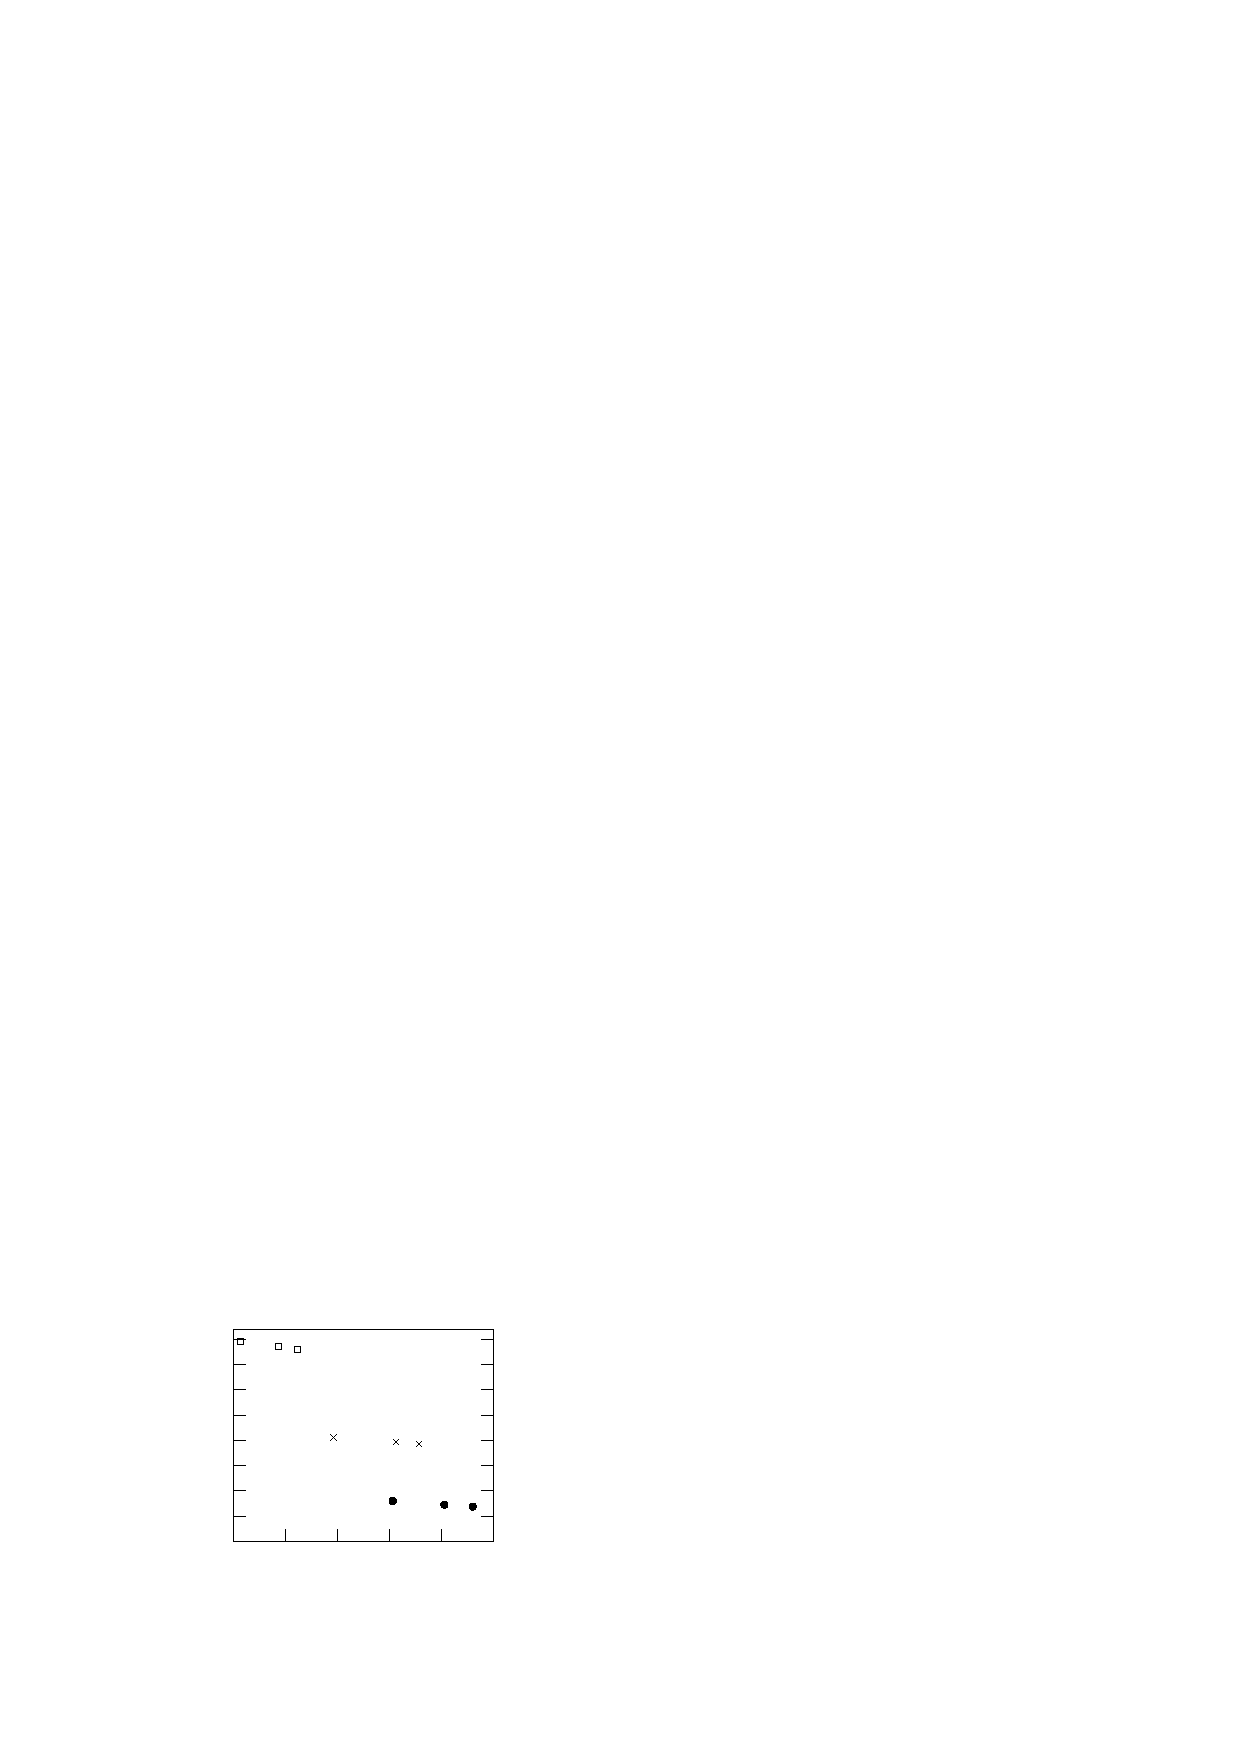
\includegraphics{reptx/reptx-bl}%
    \end{picture}%
    \begingroup
    \setlength{\unitlength}{0.0200bp}%
    \begin{picture}(9000,8100)(0,0)%
    \put(1750,1500){\makebox(0,0)[r]{\strut{} 44}}%
    \put(1750,2107){\makebox(0,0)[r]{\strut{} 44.5}}%
    \put(1750,2714){\makebox(0,0)[r]{\strut{} 45}}%
    \put(1750,3321){\makebox(0,0)[r]{\strut{} 45.5}}%
    \put(1750,3929){\makebox(0,0)[r]{\strut{} 46}}%
    \put(1750,4536){\makebox(0,0)[r]{\strut{} 46.5}}%
    \put(1750,5143){\makebox(0,0)[r]{\strut{} 47}}%
    \put(1750,5750){\makebox(0,0)[r]{\strut{} 47.5}}%
    \put(1750,6357){\makebox(0,0)[r]{\strut{} 48}}%
    \put(2000,1000){\makebox(0,0){\strut{} 8}}%
    \put(3250,1000){\makebox(0,0){\strut{} 16}}%
    \put(4500,1000){\makebox(0,0){\strut{} 32}}%
    \put(5750,1000){\makebox(0,0){\strut{} 64}}%
    \put(7000,1000){\makebox(0,0){\strut{} 128}}%
    \put(8250,1000){\makebox(0,0){\strut{} 256}}%
    \put(5125,250){\makebox(0,0){\strut{}Time (min)}}%
    \put(5125,7350){\makebox(0,0){\strut{}Normalized border length}}%
    \end{picture}%
    \endgroup
  }}
  \put(167,0){\makebox(167,145){
    %GNUPLOT: LaTeX picture with Postscript
    \begin{picture}(0,0)%
    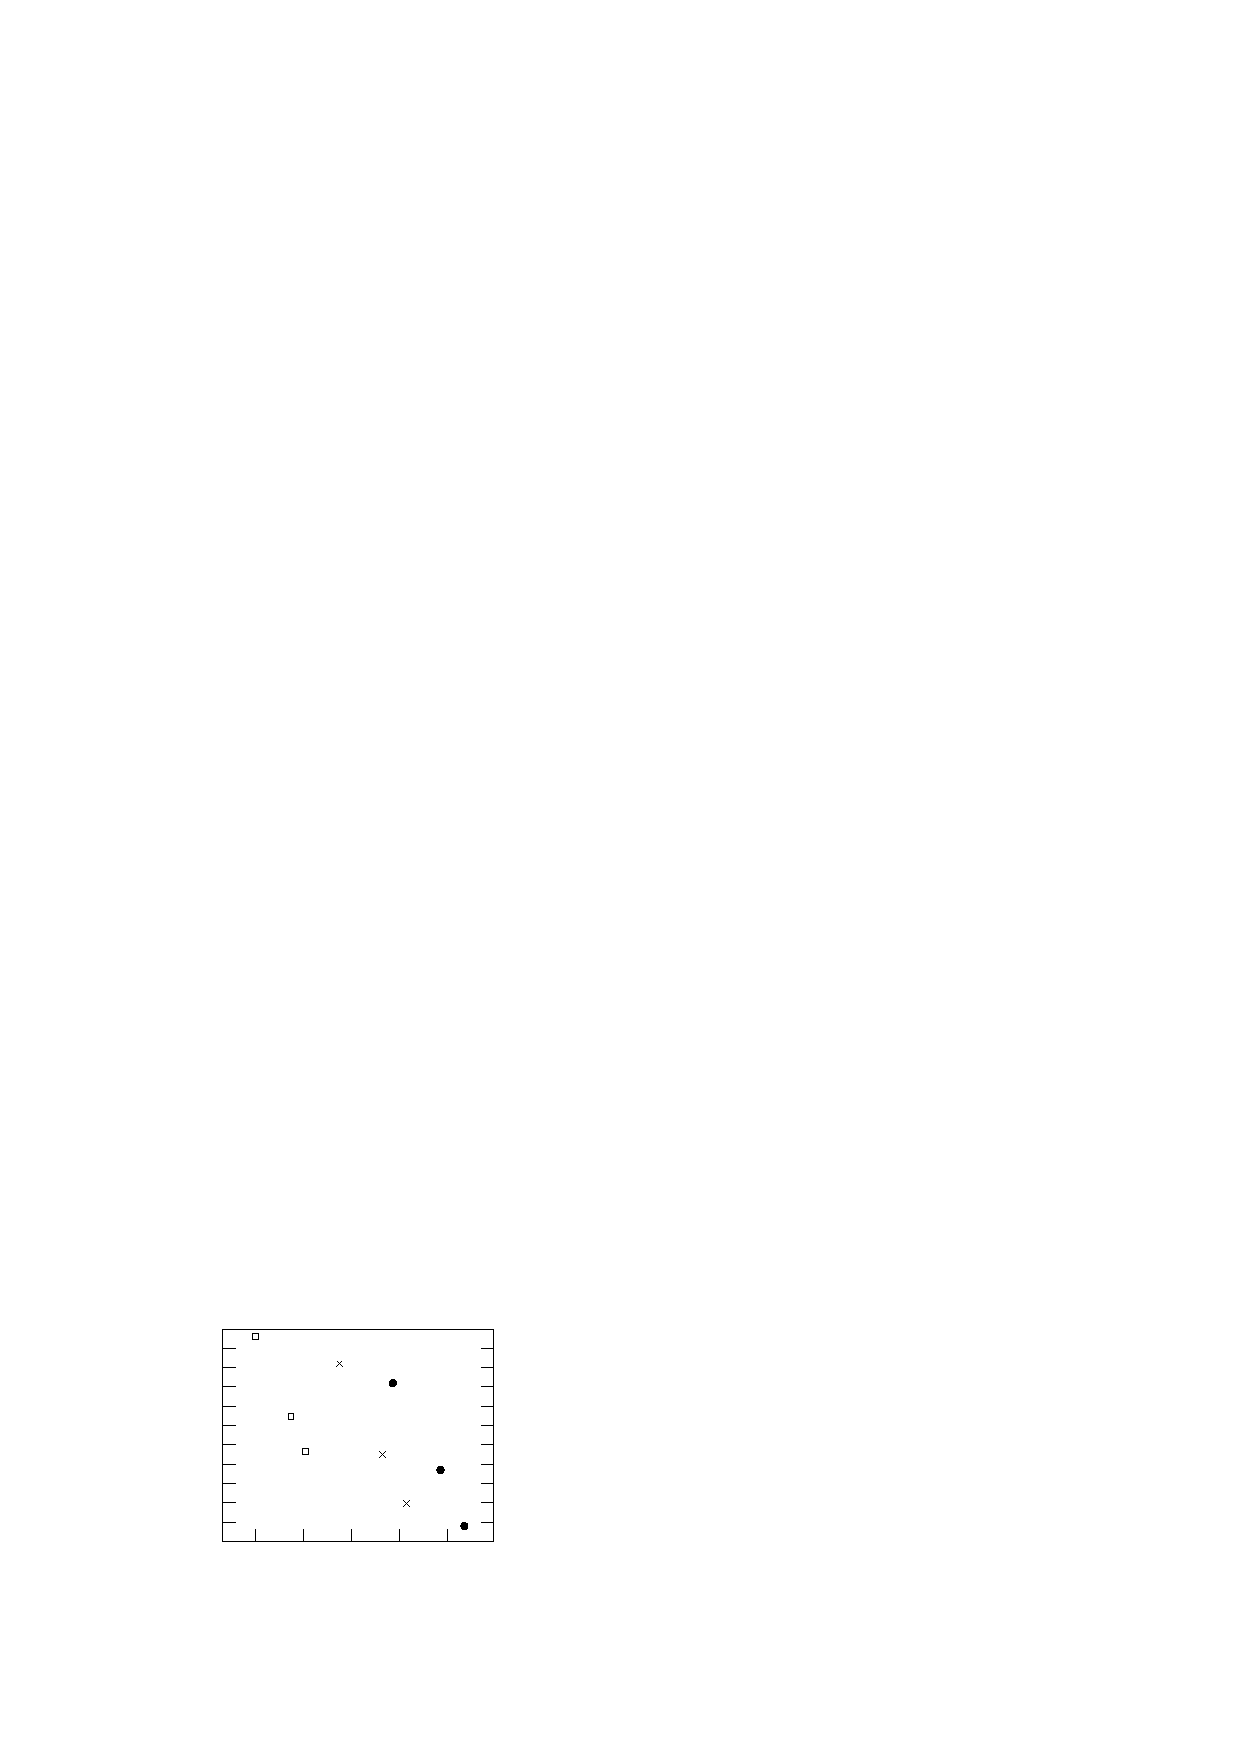
\includegraphics{reptx/reptx-ci}%
    \end{picture}%
    \begingroup
    \setlength{\unitlength}{0.0200bp}%
    \begin{picture}(9000,8100)(0,0)%
    \put(1500,1500){\makebox(0,0)[r]{\strut{} 535}}%
    \put(1500,1964){\makebox(0,0)[r]{\strut{} 540}}%
    \put(1500,2427){\makebox(0,0)[r]{\strut{} 545}}%
    \put(1500,2891){\makebox(0,0)[r]{\strut{} 550}}%
    \put(1500,3355){\makebox(0,0)[r]{\strut{} 555}}%
    \put(1500,3818){\makebox(0,0)[r]{\strut{} 560}}%
    \put(1500,4282){\makebox(0,0)[r]{\strut{} 565}}%
    \put(1500,4745){\makebox(0,0)[r]{\strut{} 570}}%
    \put(1500,5209){\makebox(0,0)[r]{\strut{} 575}}%
    \put(1500,5673){\makebox(0,0)[r]{\strut{} 580}}%
    \put(1500,6136){\makebox(0,0)[r]{\strut{} 585}}%
    \put(1500,6600){\makebox(0,0)[r]{\strut{} 590}}%
    \put(2531,1000){\makebox(0,0){\strut{} 16}}%
    \put(3683,1000){\makebox(0,0){\strut{} 32}}%
    \put(4834,1000){\makebox(0,0){\strut{} 64}}%
    \put(5986,1000){\makebox(0,0){\strut{} 128}}%
    \put(7138,1000){\makebox(0,0){\strut{} 256}}%
    \put(5000,250){\makebox(0,0){\strut{}Time (min)}}%
    \put(5000,7350){\makebox(0,0){\strut{}Average conflict index}}%
    \end{picture}%
    \endgroup
  }}
}\end{picture}
%%
\caption{\label{fig:rowepitaxial}
  Trade-off between solution quality and running time with the
  Row-Epitaxial algorithm, on random chips of dimensions $200 \times
  200$ ({\tiny $\Box$}), $300 \times 300$ ({\tiny $\times$}) and $500
  \times 500$ ({\tiny $\bullet$}).  The number $Q$ of candidates per
  spot are $10\,000$, $20\,000$, and $30\,000$ from left to right.
  Layouts are measured by normalized border length (left) and average
  conflict index (right).}
\end{figure}

%%%%%%%%%%%%%%%%%%%%%%%%%%%%%%%%%%%%%%%%%%%%%%%%%%%%%%%%%%%%%%%%%%%%%%%%%%%%%%%%
\chapter{MLP and the Quadratic Assignment Problem}
\label{ch:qap}
%%%%%%%%%%%%%%%%%%%%%%%%%%%%%%%%%%%%%%%%%%%%%%%%%%%%%%%%%%%%%%%%%%%%%%%%%%%%%%%%

In this chapter, we show that the Microarray Placement Problem (MLP) with
general distance-dependent and position-dependent weights is an instance of the
\emph{Quadratic Assignment Problem} (QAP), a classical combinatorial
optimization problem introduced by~\citet{Koopmans1957}, which opens up the way
for using QAP techniques to design microarray chips.

We then use an existing QAP heuristic algorithm called GRASP to design the
layout of small artificial chips, comparing our results with the best known
placement algorithm. The chapter ends with a discussion about how this approach
can be combined with other existing algorithms to design and improve larger
microarrays.

%%%%%%%%%%%%%%%%%%%%%%%%%%%%%%%%%%%%%%%%%%%%%%%%%%%%%%%%%%%%%%%%%%%%%%%%%%%%%%%%
\section{Quadratic assignment problem}
\label{sec:qap_qap}

The quadratic assignment problem (QAP) can be stated as follows. Given
$n \times n$ real-valued matrices $F = (f_{ij})\geq 0$ and $D = (d_{kl})\geq 0$,
find a permutation $\pi$ of $\{1, 2, \ldots n\}$ such that
\begin{equation}\label{eq:qap_def}
  \sum_{i=1}^{n} \sum_{j=1}^{n}\,  f_{ij} \cdot d_{\pi(i)\pi(j)} \to \min.
\end{equation}

The attribute \emph{quadratic} stems from the fact that the target function can
be written with $n^2$ binary indicator variables $x_{ik}\in\{0,1\}$, where
$x_{ik}:=1$ if and only if $k=\pi(i)$. The objective~(\ref{eq:qap_def}) then
becomes
%%
\[
  \sum_{i=1}^{n} \sum_{j=1}^{n}\,  f_{ij} \cdot 
  \sum_{k=1}^{n} \sum_{l=1}^{n}\,  d_{kl} \cdot x_{ik}\cdot x_{jl}
  \to \min,
\]
%%
such that $\sum_{k}\, x_{ik}=1$ for all $i$, $\sum_{i}\, x_{ik}=1$ for all $k$,
and $x_{ik}\in\{0,1\}$ for all $(i,k)$. The objective function is a quadratic
form in $x$.

The QAP has been used to model a variety of real-life problems. One common
example is the facility location problem where $n$ facilities must be assigned
to $n$ locations. The facilities could be, for instance, the clinics, doctors or
services (X-ray, emergency room, etc.) provided by a hospital and the locations
could be the available rooms of the hospital building.

In this scenario, $F$ is called the \emph{flow matrix} as $f_{ij}$ represents
the flow of materials or persons from facility $i$ to facility $j$. Matrix $D$
is called the \emph{distance matrix}, as $d_{kl}$ gives the distance between
locations $k$ and $l$. One unit of flow is assumed to have an associated cost
proportional to the distance between the facilities, and the optimal permutation
$\pi$ defines a one-to-one assignment of facilities to locations with minimum
cost.

%%%%%%%%%%%%%%%%%%%%%%%%%%%%%%%%%%%%%%%%%%%%%%%%%%%%%%%%%%%%%%%%%%%%%%%%%%%%%%%%
\section{QAP formulation of the MLP}
\label{sec:qap_mlp}

The MLP can be seen as an instance of the QAP, where we want to find a
one-to-one correspondence between spots and probes minimizing a given penalty
funtion such as total border length or total conflict index (defined in Chapter
\ref{ch:mlp}). To formulate it, we use the facility location example by viewing
the probes as locations and the spots as facilities, i.e., the spots are
assigned to the probes. The flow matrix $F$ then contains the ``closeness''
values between spots, while the distance matrix $D$ contains the conflicts
between probe embeddings.

We first give the general formulation for conflict index minimization case; the
border length minimization case is obtained by using the particular weight
functions given in Section~\ref{sec:mlp_bl_vs_ci}.

In a realistic setting, we may have more spots available than probes to place.
Below, we show that this does not cause problems as we can add enough ``empty''
probes and define their weights appropriately.

Perhaps more severely, we assume that all probes have a single pre-defined
embedding in order to force a one-to-one relationship.  A more elaborate
formulation would consider all possible embeddings of a probe, but then it
becomes necessary to ensure that only one embedding of each probe is used. This
still leads to a quadratic integer programming problem, albeit with slightly
different side conditions.

Our goal is to design a microarray minimizing the sum of conflict indices over
all spots~$s \in \CalS$, i.e.,
%%
\[
\sum_{s \in \CalS} \mathcal{C}(s) \to \min.
\]

The ``flow'' $f_{ij}$ between spots $i$ and $j$ depends on their distance on the
chip; in accordance with the conflict index model, we set
%%
\begin{equation}
  f_{ij} := \Ind{i,j \text{ neighbors}} \cdot \gamma(i,j)
\end{equation}
%%
where ``neighbors'' means that spots $i$ and $j$ are at most three cells away
(horizontally and vertically) from each other. Note that most of the flow values
on large arrays are zero. For border length minimization, the case is even
simpler: We set $f_{ij}:=1$ if spots $i$ and $j$ are adjacent, and $f_{ij}:=0$
otherwise.

The ``distance'' $d_{kl}$ between probes $k$ and $l$ depends on the conflicts
between their embeddings $\eps_k$ and $\eps_l$. To account for possible
``empty'' probes to fill up surplus spots, we set $d_{kl}:=0$ if $k$ or $l$ or
both refer to an empty probe --- i.e., empty probes never contribute to the
target function since we do not mind if nucleotides are erroneously synthesized
on spots assigned to empty probes. For real probes, we set
%%
\begin{equation}
  d_{kl} := \sum_{t=1}^{T} \Bigl(
    \Ind{\eps_{k,t}=0}
    \cdot \omega(\eps_k,t)
    \cdot \Ind{\eps_{l,t}=1} \Bigr).
\end{equation}

Note that $d_{kl}$ is related to the conflict index distance $C(k,l)$ defined in
Section~\ref{sec:mlp_conflict_index} (Equation~\ref{eq:ci_dist}):
%%
\begin{eqnarray*}
 &   & d_{kl} + d_{lk} \\
 & = & \sum_{t=1}^{T} \Bigl( \Ind{\eps_{k,t}=0} \cdot \omega(\eps_k,t) \cdot \Ind{\eps_{l,t}=1} \Bigr)
     + \sum_{t=1}^{T} \Bigl( \Ind{\eps_{l,t}=0} \cdot \omega(\eps_l,t) \cdot \Ind{\eps_{k,t}=1} \Bigr) \\
 & = & \sum_{t=1}^{T} \Bigl( \Ind{\eps_{k,t}=0 \text{ and } \eps_{l,t}=1} \cdot \omega(\eps_k,t) \Bigr)
     + \sum_{t=1}^{T} \Bigl( \Ind{\eps_{l,t}=0 \text{ and } \eps_{k,t}=1} \cdot \omega(\eps_l,t) \Bigr) \\
 & = & \sum_{t=1}^{T} \Bigl(
                        \Ind{\eps_{k,t}=0 \text{ and } \eps_{l,t}=1} \cdot \omega(\eps_k,t) +
                        \Ind{\eps_{l,t}=0 \text{ and } \eps_{k,t}=1} \cdot \omega(\eps_l,t)
                      \Bigr) \\
 & = & C(k,l)
\end{eqnarray*}

In the case of border length minimization, where $\theta=0$ and $c=1/2$ (see
Section~\ref{sec:mlp_bl_vs_ci}), we obtain that
$d_{kl} + d_{lk} = H(k,l) = H(l,k)$, where $H_{kl}$ denotes the Hamming distance
between the embeddings $\eps_k$ and $\eps_l$ (Equation~\ref{eq:hamming}).

It now follows that for a given assignment $\pi$, we have,
%%
\[
f_{ij} \cdot d_{\pi(i)\pi(j)} = \sum_{t=1}^{T} \Bigl(
  \Ind{\eps_{\pi(i),t}=0}
  \cdot \omega(\eps_{\pi(i)},t)
  \cdot \Ind{\eps_{\pi(j),t}=1}
  \cdot \Ind{i,j \text{ neighbors}}
  \cdot \gamma(i,j) \Bigr).
\]

The objective function~(\ref{eq:qap_def}) then becomes
%%
\begin{eqnarray*}
 &   & \sum_i \sum_j\, f_{ij} \cdot d_{\pi(i)\pi(j)} \\
 & = & \sum_i \sum_j\, \sum_{t=1}^{T}
                       \Bigl(
                         \Ind{\eps_{\pi(i),t}=0}
                         \cdot \omega(\eps_{\pi(i)},t)
                         \cdot \Ind{\eps_{\pi(j),t}=1}
                         \cdot \Ind{i,j \text{ neighbors}}
                         \cdot \gamma(i,j)
                       \Bigr) \\
 & = & \sum_i \sum_{t=1}^T\,
              \Bigl(
                 \Ind{\eps_{\pi(i),t}=0}
                 \cdot \omega(\eps_{\pi(i)},t)
                 \cdot \sum_j\,
                 \Ind{i,j \text{ neighbors}}
                 \cdot \Ind{\eps_{\pi(j),t}=1}
                 \cdot \gamma(i,j)
              \Bigr) \\
 & = & \sum_i \sum_{t=1}^T\,
              \Bigl(
                 \Ind{\eps_{\pi(i),t}=0}
                 \cdot \omega(\eps_{\pi(i)},t)
                 \cdot \sum_{\substack{j \text{: neighbor}\\\text{of } i}}\,
                 \Ind{\eps_{\pi(j),t}=1}
                 \cdot \gamma(i,j)
              \Bigr) \\
 & = & \sum_i \mathcal{C}(i), \\
\end{eqnarray*}
%%
and indeed equals the total conflict index with our definitions of $F=(f_{ij})$
and $D=(d_{kl})$.

\paragraph{Remark.}
Note that it is technically possible to switch the definitions of $F$ and $D$,
i.e., to assign probes to spots instead of spots to probes as we do now, without
modifying the mathematical problem formulation. However, this would lead to high
distance values for neighboring spots and many zero distance values for
independent spots, a somewhat counterintuitive model. Also, some QAP heuristics
initially find pairs of objects with large flow values and place them close to
each other. Therefore, the way of modeling $F$ and $D$ may be significant.

%%%%%%%%%%%%%%%%%%%%%%%%%%%%%%%%%%%%%%%%%%%%%%%%%%%%%%%%%%%%%%%%%%%%%%%%%%%%%%%%
\section{QAP heuristics}
\label{sec:qap_heuristics}

We have shown how the microarray placement problem can be modeled as a
quadratic assignment problem. However, the QAP is known to be NP-hard and
particularly hard to solve in practice. Instances of size larger than
$n = 20$ are generally considered to be impossible to solve to
optimality. Fortunately, several heuristics exist, including approaches based on
tabu search, simulated annealing and genetic algorithms
\citep[for a survey, see][]{Cela1997}. Our formulation is thus of interest
because we can now use existing QAP heuristics to design the layout of
microarrays minimizing either the sum of border lengths or conflict indices.

As an example, we briefly describe a general QAP heuristic known as GRASP \citep
{Li1994}, which was first used for solving the QAP by \citet{Feo1995}, and an
improved version called GRASP with path-relinking \citep{Oliveira2004}, that we
used to design small microarray chips with our formulation.

\subsection{GRASP with Path-relinking}
\label{sec:qap_grasp}

GRASP (Greedy Randomized Adaptive Search Procedure) is comprised of two phases:
a construction phase where a random feasible solution is built, and a local
search phase where a local optimum in the neighborhood of that solution is
sought. In the following description we use the terms of the facility location
problem: $f_{ij}$ is the flow between facilities $i$ and $j$, $d_{kl}$ is the
distance between locations $k$ and $l$.

The construction phase starts by sorting the $(n^2 - n)$ elements of the
distance matrix in increasing order and keeping the smallest
$E:= \lfloor \beta (n^2 - n) \rfloor$ elements, where $0 < \beta < 1$ is a
restriction parameter given as input.
%%
\begin{displaymath}
d_{k_1 l_1} \le d_{k_2 l_2} \le \cdots \le d_{k_E l_E}.
\end{displaymath}

Similarly, the $(n^2 - n)$ elements of the flow matrix are sorted, this time in
decreasing order, and the largest $E$ elements are kept:
%%
\begin{displaymath}
f_{i_1 j_1} \ge f_{i_2 j_2} \ge \cdots \ge f_{i_E j_E}.
\end{displaymath}

Then, the costs of assigning pairs of facilities to pairs of locations are
computed. The cost of initially assigning facility $i_q$ to location $k_q$ and
facility $j_q$ to location $l_q$ for some $q\in\{1,\ldots,E\}$ is
$d_{k_q l_q} f_{i_q j_q}$. GRASP sorts the vector
%%
\begin{displaymath}
(d_{k_1 l_1} f_{i_1 j_1},\;
 d_{k_2 l_2} f_{i_2 j_2},\; \ldots,\;
 d_{k_E l_E} f_{i_E j_E}),
\end{displaymath}
%%
keeping the $\lfloor \alpha E \rfloor$ smallest elements, where $0 < \alpha < 1$
is another restriction parameter. A simultaneous assignment of a pair of
facilities to a pair of locations is selected at random among those with the
$\lfloor \alpha E \rfloor$ smallest costs, and a feasible solution is then built
by making a series of greedy assignments.

In the local search phase, GRASP searches for a local optimum in the
neighborhood of the constructed solution. Several search strategies and
definitions of neighborhood can be used. One possible approach is to check every
possible swap of assignments and make only those which improve the current
solution until no further improvements can be made.

The construction and local search phases are repeated for a given number of
times, and the best solution found is returned.

\paragraph{Path-relinking.}
GRASP takes no advantage of the knowledge gained in previous iterations to
build or improve an obtained solution, i.e., each new solution is built from
scratch.

GRASP with path-relinking is an extension of the basic GRASP algorithm that uses
an ``elite set'' to store the best solutions found. It incorporates a third
phase that chooses, at random, one elite solution that is used to improve the
solution produced at the end of the local search phase.

Solutions $p$ and $q$ are combined as follows. For every location
$k = 1, \ldots, n$, the path-relinking algorithm attempts to exchange facility
$p_k$ assigned to location $k$ in  solution $p$ with facility $q_k$ assigned to
location $k$ in the elite solution. In order to keep the solution $p$ feasible,
it exchanges $p_k$ with $p_l$, where $p_l = q_k$. This exchange is performed
only if it results in a better solution. The result of the path-relinking phase
is a solution $r$ that is at least as good as the better of $p$ and $q$.

%%%%%%%%%%%%%%%%%%%%%%%%%%%%%%%%%%%%%%%%%%%%%%%%%%%%%%%%%%%%%%%%%%%%%%%%%%%%%%%%
\section{Results}
\label{sec:qap_results}

We present experimental results of using GRASP with path-relinking (GRASP-PR)
for designing the layout of small artificial chips, and compare them with the
layouts produced by the Greedy placement algorithm (described in
Section~\ref{sec:placement_greedy}), with the number $Q$ of candidates per spot
set to a sufficiently large value so that all available probes are considered
for each spot.

We used a C implementation of GRASP-PR provided by \citet{Oliveira2004} with
default parameters (32 iterations, $\alpha=0.1$, $\beta=0.5$, and elite set of
size $10$). The main routine takes three arguments: the dimension $n$ of the
problem (in our case, the number of spots or probes) and matrices $F$ and $D$.
The matrices were generated using the formulations presented in Section
\ref{sec:qap_mlp}.

The data set consists of chips with probes of length 25 uniformly generated and
asynchronously embedded in a deposition sequence of length 74. The running times
and the border lengths of the resulting layouts are shown in
Table~\ref{tab:graspr_greedy_bl} (all results are averages over a set of ten
chips).

\begin{table}[t]\centering
\caption{\label{tab:graspr_greedy_bl}
  Total border length of random chips compared with the layouts produced by
  Greedy and GRASP with path-relinking. Reductions in border length are reported
  in percentages compared to the random layout.}
\footnotesize{
\begin{tabular}{crcrrrcrrr}
          & Random & & \multicolumn{3}{c}{Greedy placement}  & & \multicolumn{3}{c}{GRASP with path-relinking}  \\ \cline{2-2} \cline{4-6} \cline{8-10}
Chip      & Border & & Border & Reduction & Time             & & Border & Reduction & Time   \\
dimension & length & & length & (\%)      & (sec.)           & & length & (\%)      & (sec.) \\
\hline
$6\times 6$   & 1\,989.20 & & 1\,714.60 & 13.80 & 0.01 & & 1\,672.20 & 15.94 &   2.73 \\
$7\times 7$   & 2\,783.20 & & 2\,354.60 & 15.40 & 0.02 & & 2\,332.60 & 16.19 &   6.43 \\
$8\times 8$   & 3\,721.20 & & 3\,123.80 & 16.05 & 0.03 & & 3\,099.13 & 16.72 &  12.49 \\
$9\times 9$   & 4\,762.00 & & 3\,974.80 & 16.53 & 0.05 & & 3\,967.20 & 16.69 &  25.96 \\
$10\times 10$ & 5\,985.20 & & 4\,895.60 & 18.20 & 0.06 & & 4\,911.40 & 17.94 &  47.57 \\
$11\times 11$ & 7\,288.40 & & 5\,954.40 & 18.30 & 0.10 & & 5\,990.73 & 17.80 &  87.48 \\
$12\times 12$ & 8\,714.00 & & 7\,086.20 & 18.68 & 0.11 & & 7\,159.80 & 17.84 & 152.42 \\
\hline
\end{tabular}}
\end{table}

Our results show that GRASP-PR produces layouts with lower border lengths than
Greedy on the smaller chips. On $6\times 6$ chips, GRASP-PR outperforms Greedy
by $2.14$ percentage points on average ($15.94\% - 13.80\%$), when compared to
the initial random layout. On $9\times 9$ chips, however, this difference drops
to $0.16$ percentage points, while Greedy generates better layouts on
$11\times 11$ or larger chips. In terms of running time, Greedy is faster and
shows little variation as the number of probes grows. In contrast, the time
required to compute a layout with GRASP-PR increases at a fast rate.

Table~\ref{tab:graspr_greedy_ci} shows better results in terms of conflict
indices. GRASP-PR consistently produces better layouts on all chip dimensions,
achieving up to $6.38$\% less conflicts on $10\times 10$ chips, for example,
when compared to Greedy. In terms of running times, GRASP-PR is even slower than
in the border length case. The reason is not clear, but it could be because the
distance matrix contains fewer zero entries with the conflict index formulation.

The gains in terms of conflict index of both Greedy and GRASP-PR are clearly
less than the gains in terms of border length (when compared to the initial
random layout). This may be because the probe embeddings are fixed and the
reduction of conflicts is restricted to the relocation of the probes, which only
accounts for one part of the conflict index model.

\begin{table}[t]\centering
\caption{\label{tab:graspr_greedy_ci}
  Average conflict indices of random chips compared with the layouts produced by
  Greedy and GRASP with path-relinking.}
\footnotesize{
\begin{tabular}{crcrrrcrrr}
          & Random & & \multicolumn{3}{c}{Greedy placement}  & & \multicolumn{3}{c}{GRASP with path-relinking}  \\ \cline{2-2} \cline{4-6} \cline{8-10}
Chip      & Avg. C.& & Avg. C.& Reduction & Time             & & Avg. C.& Reduction & Time   \\
dimension & Index  & & Index  & (\%)      & (sec.)           & & Index  & (\%)      & (sec.) \\
\hline
$6\times 6$   & 524.28 & & 495.15 & 5.56 & 0.05 & & 467.08 & 10.91 &   3.68 \\
$7\times 7$   & 558.25 & & 521.90 & 6.51 & 0.07 & & 489.32 & 12.35 &   8.84 \\
$8\times 8$   & 590.51 & & 551.84 & 6.55 & 0.09 & & 515.69 & 12.67 &  19.48 \\
$9\times 9$   & 613.25 & & 568.62 & 7.28 & 0.11 & & 533.79 & 12.96 &  38.83 \\
$10\times 10$ & 628.50 & & 576.49 & 8.28 & 0.11 & & 539.69 & 14.13 &  73.09 \\
$11\times 11$ & 642.72 & & 588.91 & 8.37 & 0.12 & & 551.41 & 14.21 & 145.67 \\
$12\times 12$ & 656.86 & & 598.21 & 8.93 & 0.12 & & 561.21 & 14.56 & 249.19 \\
\hline
\end{tabular}}
\end{table}

%%%%%%%%%%%%%%%%%%%%%%%%%%%%%%%%%%%%%%%%%%%%%%%%%%%%%%%%%%%%%%%%%%%%%%%%%%%%%%%%
\section{Discussion}
\label{sec:qap_discussion}

The QAP is notoriously hard to solve, and currently known exact methods start to
take prohibitively long already for slightly more than $20$ objects, i.e., we
could barely solve the problem exactly for $5\times 5$ arrays. Fortunately, the
literature on QAP heuristics is rich, as many problems in operations research
can be modeled as QAPs. Here we used one such heuristic to identify the
potential of the MLP-QAP-relation.

As our results show, however, even heuristic algorithms are too slow to deal
with chips of dimensions larger than $12 \times 12$, and although we could
design a $20 \times 20$ chip with a QAP heuristic within a day, we have to keep
in mind that this would still be a very small part of bigger problem as real
microarray dimensions range from $200 \times 200$ up to $1164 \times 1164$.

For this reason, we restricted our experiments to such small chips and QAP
heuristics that could handle the problems within a few minutes. Up to now,
finding exact solutions even to these small microarrays seems to be an
incredible hard task. We mention here experiments conducted by Dr. Peter Hahn,
who used two branch-and-bound algorithms to solve some problem instances from
Table \ref{tab:graspr_greedy_bl}. With RTL-2 \citep{Adams}, it was possible to
find two solutions with total border length of $1\,652$ for a selected
$6\times 6$ chip, being only $1.43\%$ better than the solution found with GRASP-
PR ($1\,676$), although it took RTL-2 about $6.5$ hours, in contrast with the
less than 3 seconds needed by GRASP-PR. A lower bound calculation for the same
problem resulted in $1\,624$, so the RTL-2 solution is only $1.69\%$ higher,
while the gap to the GRASP-PR solution is about $3.10\%$.

For another selected problem of dimension $7\times 7$, Dr. Hahn found one
solution with border length $2\,290$ using RTL-1 \citep{Hahn1998}, being about
$1.72\%$ better than the solution found by GRASP-PR ($2\,330$), although it took
RTL-1 some 29 hours, in contrast with the less than 7 seconds needed for the
GRASP-PR run. The results obtained with exact QAP solvers give an idea of how
hard the quadratic assignment problem actually is, and show that the results
with GRASP-PR are a good compromise when time is limited.

Improved results for several selected problem instances from Tables
\ref{tab:graspr_greedy_bl} and \ref{tab:graspr_greedy_ci} were also reported by
Chris MacPhee using GATS, a hybrid genetic / tabu search algorithm, although
these results were obtained on a number of large memory SMP machines, each
having 144 processors and 576 GB of global memory. The latest results for these
selected problems are available online at \url{
http://gi.cebitec.uni-bielefeld.de/assb/chiplayout/qap}.

\subsection{Alternatives}

It is clear that, because of the large number of probes on industrial
microarrays, it is not feasible to use GRASP-PR (or any other currently
available QAP method) to design an entire microarray chip. However, we showed
that it is certainly possible to use it on small sub-regions of a chip, which
opens up the way for two alternatives.

First, the QAP approach could be used combined with a partitioning algorithm
such as those discussed in Chapter \ref{ch:part} to the design the smaller
regions that result from the partitioning. This, however, does not seem
promising because, as we will see later, a partitioning is a compromise in
solution quality, and level of partitioning required to achieve the dimensions
supported by the QAP approach is too high.

It is interesting to extrapolate the times shown on Table
\ref{tab:graspr_greedy_bl} to predict the total time that would be required to
design the layout of commercial microarrays, if we were to combine GRASP-PR with
a partitioning algorithm. If the partitioning produced $6\times 6$ regions,
$37\,636$ sub-regions would be created from the $1164\times 1164$ Affymetrix
Human Genome U133 Plus 2.0 GeneChip array, one of the largest Affymetrix chips.
Since each sub-region takes around 3 seconds to compute with GRASP-PR, the total
time required for designing such a chip would be a little over 31 hours
(ignoring the time for the partitioning itself).

If the partitioning produced $12\times 12$ regions, $9\,409$ sub-regions would
be created and, at 2.4 minutes each, the total time would be more than 16 days.
This is probably prohibitive, although it is certainly possible to reduce the
time of each GRASP-PR execution by running it on faster machines or run them in
parallel.

A better alternative is to use the QAP approach to improve an existing layout,
iteratively, by relocating probes inside a defined region of the chip, in a
sliding-window fashion. Each iteration of this method would produce an instance
of a QAP whose size equals the number of spots inside the window.The QAP
heuristics could then be used to check whether a different arrangement of the
probes inside the window can reduce the conflicts. For this approach to work,
however, we also need to take into account the conflicts due to the spots around
the window. Otherwise, a new layout with less internal conflicts could be
achieved at the expense of increasing conflicts on the borders of the window.

A simple way of preventing this problem is to solve a larger QAP instance
consisting of the spots inside the window as well as those in a layer (of three
spots) around it. The spots outside the window obviously must remain unchanged,
and that can be done by fixing the corresponding elements of the permutation
$\pi$. Note that there is no need to compute $f_{ij}$ if spots $i$ and $j$ are
both outside the window, nor $d_{kl}$ if probes $k$ and $l$ are assigned to
spots outside the window.


%%%%%%%%%%%%%%%%%%%%%%%%%%%%%%%%%%%%%%%%%%%%%%%%%%%%%%%%%%%%%%%%%%%%%%%%%%%%%%%%
\chapter{Re-embedding Algorithms}
\label{ch:reembed}
%%%%%%%%%%%%%%%%%%%%%%%%%%%%%%%%%%%%%%%%%%%%%%%%%%%%%%%%%%%%%%%%%%%%%%%%%%%%%%%%

After the placement phase, it is no longer possible to reduce conflicts if
probes are synchronously embedded. With asynchronous embeddings, however,
layouts can usually be further improved by \emph{re-embedding} the probes
without changing their locations on the chip, in what is sometimes called a
\emph{post-placement optimization} phase.

All re-embedding algorithms discussed in this chapter are based on the Optimum
Single Probe Embedding (OSPE) introduced by \citet{Kahng2002}. OSPE is a dynamic
programming algorithm for computing an optimum embedding of a single probe with
respect to its neighbors, whose embeddings are considered as fixed. The
algorithm was originally developed for border length minimization (BLM) but here
we present a more general form designed for conflict index minimization (CIM)
that first appeared in \citep{Carvalho2006}.

\section{Optimum Single Probe Embedding}
\label{sec:reembed_ospe}

The Optimum Single Probe Embedding algorithm, OSPE for short, can be seen as a
special case of a global alignment between a probe sequence $p$ of length $\ell$
and the deposition sequence $N$ of length $T$, disallowing mismatches and gaps
in $N$. We assume that $p$ is placed at spot $s$, and that we know the
embeddings of all probes placed at spots near $s$ (spots that are at most three
cells away from $s$, horizontally and vertically, in accordance with the
conflict index model).

The optimal embedding of $p$ into $N$ is built by determining the minimum cost
of embedding a prefix of $p$ into a prefix of $N$: We use an
$(\ell + 1) \times (T + 1)$ matrix $D$, where $D[i,t]$ is defined as the minimum
cost of an embedding of $p[1..i]$ into $N[1..t]$. The cost is the sum of
conflicts induced by the embedding of $p[1..i]$ on its neighbors (when $s$ is
unmasked and a neighbor is masked), plus the conflicts suffered by $p[1..i]$
because of the embeddings of its neighbors (when $s$ is masked and a neighbor is
unmasked).

We can compute the value for $D[i,t]$ by looking at two previous entries in the
matrix: $D[i,t-1]$ and $D[i-1,t-1]$. The reason is that $D[i,t]$ is the minimum
cost of embedding $p[1..i]$ up to the $t$-th synthesis step of $N$, which can
only be obtained from the previous synthesis step ($t-1$) by either masking or
unmasking spot~$s$ at step~$t$.

If $s$ is productive (unmasked) at step $t$, base $N_t$ is appended to
$p[1..i-1]$; this is only possible if $p[i]=N[t]$. In this case a cost $U_t$ is
added for the risk of damaging probes at neighboring spots $s'$. We know that
$p[1..i-1]$ can be embedded in $N[1..t-1]$ with optimal cost $D[i-1,t-1]$.
Hence, the minimum cost at step $t$, if $s$ is productive, is $D[i-1,t-1] +
U_t$.  According to the conflict index model,
\[
U_t := \sum_{\substack{s'\text{: neighbor}\\\text{of } s}}
  \Ind{\eps_{k(s'),t}=0}
  \cdot \omega(\eps_{k(s')},t)
  \cdot \gamma(s',s).
\]

If $s$ is unproductive (masked) at step $t$, no base is appended to $p[1..i]$,
but a cost $M_{i,t}$ must be added for the risk of damaging $p$ (by light
directed at neighboring spots $s'$). Since $D[i,t-1]$ is the minimum cost of
embedding $p[1..i]$ in $N[1..t-1]$, the minimum cost up to step $t$, if $s$ is
unmasked, is $D[i,t-1] + M_{i,t}$.

Note that $M_{i,t}$ depends on the number of bases $p$ already contains (that
is, on $i$): Each unmasked neighbor $s'$ generates a conflict on $p$ with cost
\[
\gamma(s,s') \cdot c \cdot \exp[\theta\cdot (1+\min\{i,\ell-i\})],
\]
in accordance with (\ref{eq:pos_mult})--(\ref{eq:b_ell}). Thus,
\[
M_{i,t} := c \cdot \exp[\theta\cdot (1+\min\{i,\ell-i\})] \cdot
\sum_{\substack{s'\text{: neighbor}\\\text{of } s}}
\Ind{\eps_{k(s'),t}=1}  \cdot \gamma(s,s').
\]

Finally, $D[i,t]$ is computed as the minimum cost of the possible actions,
\[
D[i,t] := \begin{cases}
  \min \{\, D[i,t-1] + M_{i,t},\;  D[i-1,t-1] + U_t \,\}
  & \text{ if $p[i]=N[t]$,}\\
  D[i,t-1] + M_{i,t}
  & \text{ if $p[i]\neq N[t]$.}
  \end{cases}
\]

The first column of $D$ is initialized as follows: $D[0,0] = 0$ and
$D[i,0] = \infty$ for $0 < i \leq \ell$, since no probe of length $\ell > 0$ can
be embedded into an empty deposition sequence. The first row is initialized by
setting $D[0,t] = D[0,t-1]+M_{0,t}$ for $0<t\leq T$.

If we assume that costs $U_t$ and $M_{i,t}$ can be computed in constant time,
the time complexity of the OSPE algorithm is $O(\ell T)$ since there are
$O(\ell T)$ entries in $D$ to compute. The algorithm can be rather
time-consuming in the general form presented here, since we have to look at the
embeddings of up to 48 neighbors around~$s$. Naturally, it runs much faster for
border length minimization, since there are only four neighbors to look at, and
there are neither position-dependent ($\omega$) nor distance-dependent
($\gamma$) weights to compute. In practice, a simple optimization can
significantly reduce running time: in each row, only the columns between the
left-most and right-most embeddings of $p$ in $N$ need to be computed (see
Figure~\ref{fig:ospe}).

\begin{figure}[t]\centering
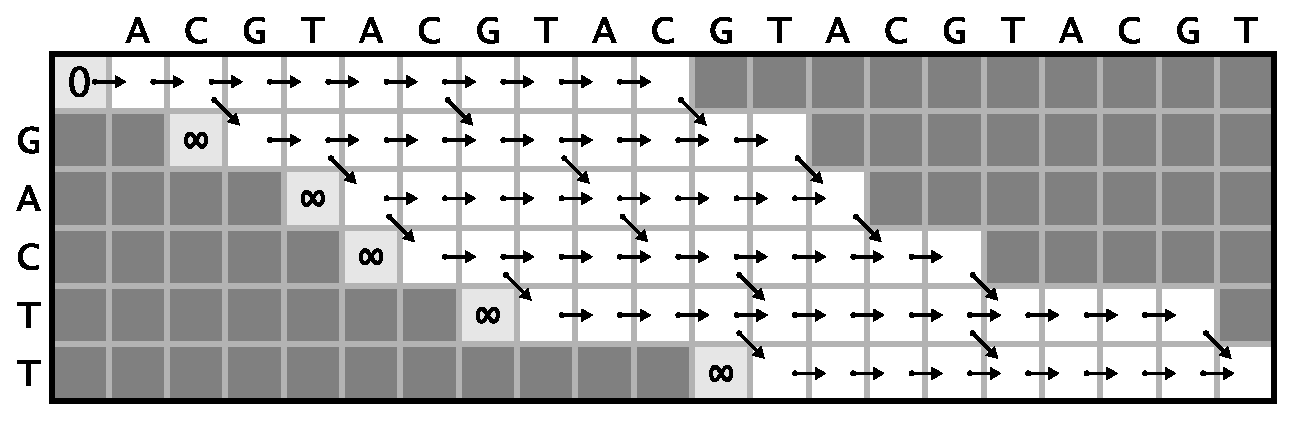
\includegraphics[width=\textwidth]{reembed/ospe}
\caption{\label{fig:ospe}%
  OSPE's dynamic programming matrix for computing an optimal embedding of a
  probe $p=\text{GACTT}$ in a deposition sequence $N=\text{\{ACGT\}}^5$. Dark
  shaded cells are not computed. Arrows show all paths in the matrix leading to
  a valid embedding of $p$ in $N$.}
\end{figure}

Once $D$ is computed, the minimum cost is $D[\ell,T]$, and an optimal embedding
of $p$ in $N$ can be constructed by tracing a path from $D[\ell,T]$ back to
$D[0,0]$, similarly to the procedure used to build an optimal global alignment.
This takes $O(T)$ time.

The OSPE algorithm is the basic operation of several post-placement optimization
algorithms: Chessboard, Greedy and Batched Greedy, Sequential as well as our new
Priority re-embedding algorithm. The main difference between these algorithms
lies in the order in which the probes are re-embedded.

Since OSPE never increases the amount of conflicts in the region around the
re-embedded probe, optimization algorithms can execute several re-embedding
operations without risk of worsening the current layout. Moreover, each probe
may be re-embedded several times since new improvements may be possible once its
neighbors have been changed. In fact, all algorithms presented here work in
repeating cycles of optimization until no more improvements are possible (when a
local optimal solution is found), until improvements drop below a given
threshold $W$, or until a given number of cycles (or \emph{passes}) have been
executed.

%%%%%%%%%%%%%%%%%%%%%%%%%%%%%%%%%%%%%%%%%%%%%%%%%%%%%%%%%%%%%%%%%%%%%%%%%%%%%%%%
\section{Chessboard}
\label{sec:reembed_chessboard}

The Chessboard re-embedding algorithm \citep{Kahng2002} was initially designed
for border length minimization, and it takes advantage of the fact that, in this
model, a chip can be bi-colored like a chessboard, in such a way that the
embeddings of probes located on white spots are independent of those placed on
black spots (Figure~\ref{fig:chessboard}a).

Chessboard uses this coloring to alternate the optimal re-embedding of probes
located on black and white spots with respect to their neighbors: Each pass of
Chessboard consists of re-embedding all probes of black spots and then all probe
of white spots.

The chessboard coloring guarantees that probes re-embedded in the same step are
independent with respect to the border length model, i.e. they can be
re-embedded without affecting the border conflicts of other spots with the same
color. For conflict index minimization, the same principle can be applied by
using $4\times 4=16$ colors instead of~$2$ as illustrated in
Figure~\ref{fig:chessboard} (to the best of our knowledge this has not yet been
implemented).

\begin{figure}[t]\centering
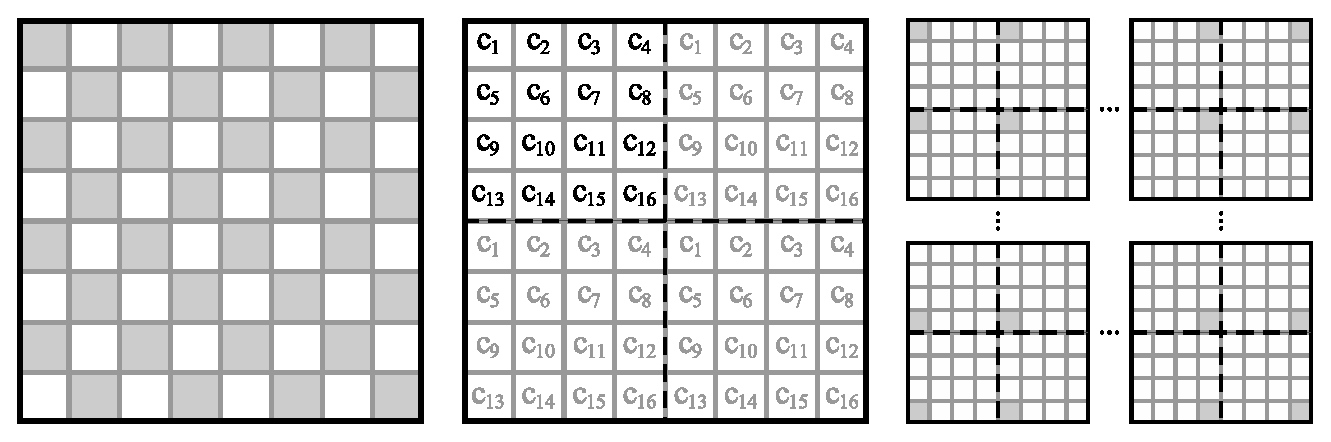
\includegraphics[width=\textwidth]{reembed/chessboard}
\begin{picture}(435,20)
\put(-3,0){ \makebox(136,20){a)}}
\put(150,0){\makebox(137,20){b)}}
\put(301,0){\makebox(136,20){c)}}
\end{picture}
\caption{\label{fig:chessboard}%
  a) The chessboard-like bi-coloring of a chip used by the Chessboard
  re-embedding algorithm for border length minimization; b) a possible coloring
  of the chip for conflict index minimization using 16 colors
  ($c_1 \dots c_{16}$), resulting in sets of independent spots; c) four of the
  16 sets of independent spots (shaded) that can be re-embedded in the same
  iteration.}
\end{figure}

%%%%%%%%%%%%%%%%%%%%%%%%%%%%%%%%%%%%%%%%%%%%%%%%%%%%%%%%%%%%%%%%%%%%%%%%%%%%%%%%
\section{Greedy and Batched Greedy}
\label{sec:reembed_greedy}
  
As its name implies, the Greedy re-embedding algorithm \citep{Kahng2002}
utilizes a greedy strategy for choosing the order in which probes are
re-embedded. At each iteration, Greedy examines every spot of the chip and
computes the maximum reduction of border conflicts achievable by optimally
re-embedding its probe. It then selects a spot with the highest gain (reduction
of conflicts) and re-embeds its probe optimally, updating the gains of adjacent
spots.

A faster version of this algorithm, called Batched Greedy \citep{Kahng2002},
pre-selects several independent spots for re-embedding and thus sacrifices its
greedy nature in favour of running time by postponing the update of gains.

Like Chessboard, Greedy and Batched Greedy were initially developed for border
length minmization, but they can also be extended for conflict index
minimization. The main difference is that, once a probe is re-embedded, more
neighbors need to be updated. For Batched Greedy, the selection of independent
spots need to take into account the minimum distance of four cells (horizonally
and vertically) between spots, in accordance with the conflict index model
(Section~\ref{sec:mlp_conflict_index}). Hence fewer spots may be be re-embedded
in the same iteration.

%%%%%%%%%%%%%%%%%%%%%%%%%%%%%%%%%%%%%%%%%%%%%%%%%%%%%%%%%%%%%%%%%%%%%%%%%%%%%%%%
\section{Sequential re-embedding}
\label{sec:reembed_sequential}

The Sequential algorithm \citep{Kahng2003a} employs a much simpler and,
surprisingly, more efficient strategy. The algorithm just proceeds spot by spot,
from top to bottom, left to right, re-embedding each probe optimally in regards
to its neighbors. Once the end of the array is reached, Sequential restarts at
the top left of the array for the next iteration.

The algorithm is not only simple but also fast since there is no need to compute
achievable gains for each spot. Nonetheless, Sequential achieved the greatest
reduction of border conflicts in the experiments of \citet{Kahng2003a}. The
authors argue that the main shortcoming of Chessboard and Greedy is that they
always re-embed an independent set of spots at a time, and dropping this
requirement should allow faster propagation of the effects of new embeddings and
hence convergence to a better local optimum.

Tables \ref{tab:sequential_bl} and \ref{tab:sequential_ci} show the results of
using Sequential to re-embed the probes of chips produced by the Greedy
placement algorithm (Section~\ref{sec:placement_greedy}). The chips initially
contained random probes of length 25, uniformly generated, and left-most
embedded in the standard Affymetrix deposition sequence.
The threshold $W$ was set to $0.2\%$ (Sequential stopped as soon as the total
reduction of conflicts in one pass droped below $0.2\%$). In all cases, the
threshold was reached after two passes.

\begin{table}[t]\centering
\caption{\label{tab:sequential_bl}
  Normalized border length (NBL) before and after an optimization phase with the
  Sequential re-embedding algorithm. Placement was produced by the Greedy
  placement algorithm (Section~\ref{sec:placement_greedy}) with border length
  minimization, $0$-threading, and number $Q$ of candidates per spot set to 5K
  and 20K. The average number of passes executed by Sequential before the
  threshold $W=0.2\%$ was reached is shown. The reduction of conflicts is also
  shown in percentage. Running times are reported in seconds and all results are
  averages over a set of five chips. The time spent by Sequential is also shown
  as a percentage of the total time (placement plus re-embedding).}
\footnotesize{
\begin{tabular}{crrrlrrrrr}
\vspace{1pt}
     & \multicolumn{3}{c}{Greedy placement} & & \multicolumn{5}{c}{Sequential re-embedding} \\ \cline{2-4} \cline{6-10}
\vspace{1pt}
Dim. & $Q$ & NBL & Time & & NBL & Reduct. & Passes & Time & \%Total time \\
\hline
$300\times 300$ &  5K & 18.3182 &     98.5 & & 18.2121 & 0.579\% & 2.0 &  4.8 & 4.617\% \\
                & 20K & 18.0576 &    577.9 & & 17.9726 & 0.471\% & 2.0 &  4.8 & 0.830\% \\
\hline
$500\times 500$ &  5K & 17.5830 &    345.7 & & 17.4851 & 0.557\% & 2.0 & 12.7 & 3.538\% \\
                & 20K & 17.3554 & 1\,999.8 & & 17.2779 & 0.446\% & 2.0 & 12.6 & 0.625\% \\
\hline
$800\times 800$ &  5K & 16.9124 &    916.8 & & 16.8201 & 0.546\% & 2.0 & 32.6 & 3.437\% \\
                & 20K & 16.6980 & 5\,749.7 & & 16.6258 & 0.432\% & 2.0 & 32.4 & 0.560\% \\
\hline
\end{tabular}}
\end{table}

\begin{table}[ht]\centering
\caption{\label{tab:sequential_ci}
  Average conflict index (ACI) before and after an optimization phase with the
  Sequential re-embedding algorithm with $W=0.2\%$. Placement was produced by
  the Greedy placement algorithm with conflict index minimization,
  $0$-threading, and $Q$ set to 5K and 20K.}
\footnotesize{
\begin{tabular}{crrrlrrrrr}
\vspace{1pt}
     & \multicolumn{3}{c}{Greedy placement} & & \multicolumn{5}{c}{Sequential re-embedding} \\ \cline{2-4} \cline{6-10}
\vspace{1pt}
Dim. & $Q$ & ACI & Time & & ACI & Reduct. & Passes & Time & \%Total time \\
\hline
$300\times 300$ &  5K & 440.5166 &     322.4 & & 436.8630 & 0.829\% & 2.0 &    188.9 & 36.944\% \\
                & 20K & 415.5003 &  1\,818.6 & & 412.5536 & 0.709\% & 2.0 &    189.9 &  9.457\% \\
\hline
$500\times 500$ &  5K & 432.3023 &     952.5 & & 428.7410 & 0.824\% & 2.0 &    527.3 & 35.632\% \\
                & 20K & 401.4609 &  4\,027.2 & & 398.6096 & 0.710\% & 2.0 &    528.3 & 11.597\% \\
\hline
$800\times 800$ &  5K & 426.0757 &  2\,512.1 & & 422.6277 & 0.809\% & 2.0 & 1\,357.9 & 35.087\% \\
                & 20K & 392.1786 & 11\,182.8 & & 389.3929 & 0.710\% & 2.0 & 1\,352.5 & 10.790\% \\
\hline
\end{tabular}}
\end{table}

The reduction of conflicts achieved by Sequential were small (at most $0.579\%$
with border length and $0.829\%$ for CIM), which shows that there is little room
for improvements once the placement is fixed. In fact, the more time is spent
during placement (greater $Q$), the less reduction of conflicts is achieved by
re-embedding. For instance, on a $300\times 300$ chip, the reduction in average
conflict index dropped by $0.12$ percentage point (from $0.829\%$ to $0.709\%$)
when the number of candidades per spot considered by Greedy during placement was
increased from 5K to 20K.

Although the reductions of conflicts were relatively small, Sequential required
approximately half a minute to re-embedded (two times) all probes of a
$800\times 800$ chip in the BLM case, which represented about $3.44\%$ of the
aggregate time (placement and re-embedding) when $Q=5$K and only $0.56\%$ when
$Q=20$K.

In some cases, Sequential even provided comparable reduction of border
conflicts, in less time, than increasing $Q$ for Greedy. For instance, on a
$800\times 800$ chip, Greedy placement with $Q=20$K and two passes of Sequential
re-embedding produced, in approximately half of the time, a layout with only
$0.14\%$ more border conflicts than Greedy with $Q=40$K and no re-embedding
($16.6258$ NBL in $96.4$ minutes versus $16.6026$ in $189.0$ minutes,
respectively; data not shown).

Figure~\ref{fig:sequential-bl_blm} shows the normalized border length per
masking step of a selected $500\times 500$ chip before and after a re-embedding
phase with Sequential for BLM. It is clear that the reduction of conflicts is
achieved mainly between steps 45 and 65, at the expense of a small increase in
conflicts in the final synthesis steps. This is a result of fixing the placement
with left-most embedded probes, which leaves no room for improvements in the
first masks.

In terms of CIM, the reductions were slightly higher but Sequential was over 40
times slower than in the BLM case, taking up to $36.9\%$ of the aggregate time.
This, coupled with the fact that Greedy gives significant reductions of
conflicts with increasing $Q$ even beyond 40K, makes it difficult to justify the
time spent with re-embedding, unless when $Q$ is approaching its limit (number
of probes on the chip) and one is looking for the best layout possible.

Figure~\ref{fig:sequential-ci_blm} shows the normalized border length per
masking step of the same $500\times 500$ chip of
Figure~\ref{fig:sequential-bl_blm} before and after a re-embedding phase with
Sequential for CIM (placement was produced by Greedy also for CIM). Again,
reduction of conflicts is restricted to the second half of synthesis steps
because of the left-most embeddings, although with relatively better
improvements when compared with the border length case.

Our results also confirm that Sequential has a linear time complexity (if we
consider that each OSPE operation can be done in constant time). Sequential
performed around $19\,400$ re-embeddings per second in the BLM case and around
$475$ re-embeddings per second in the CIM case, on average.

\begin{figure}[t]\centering
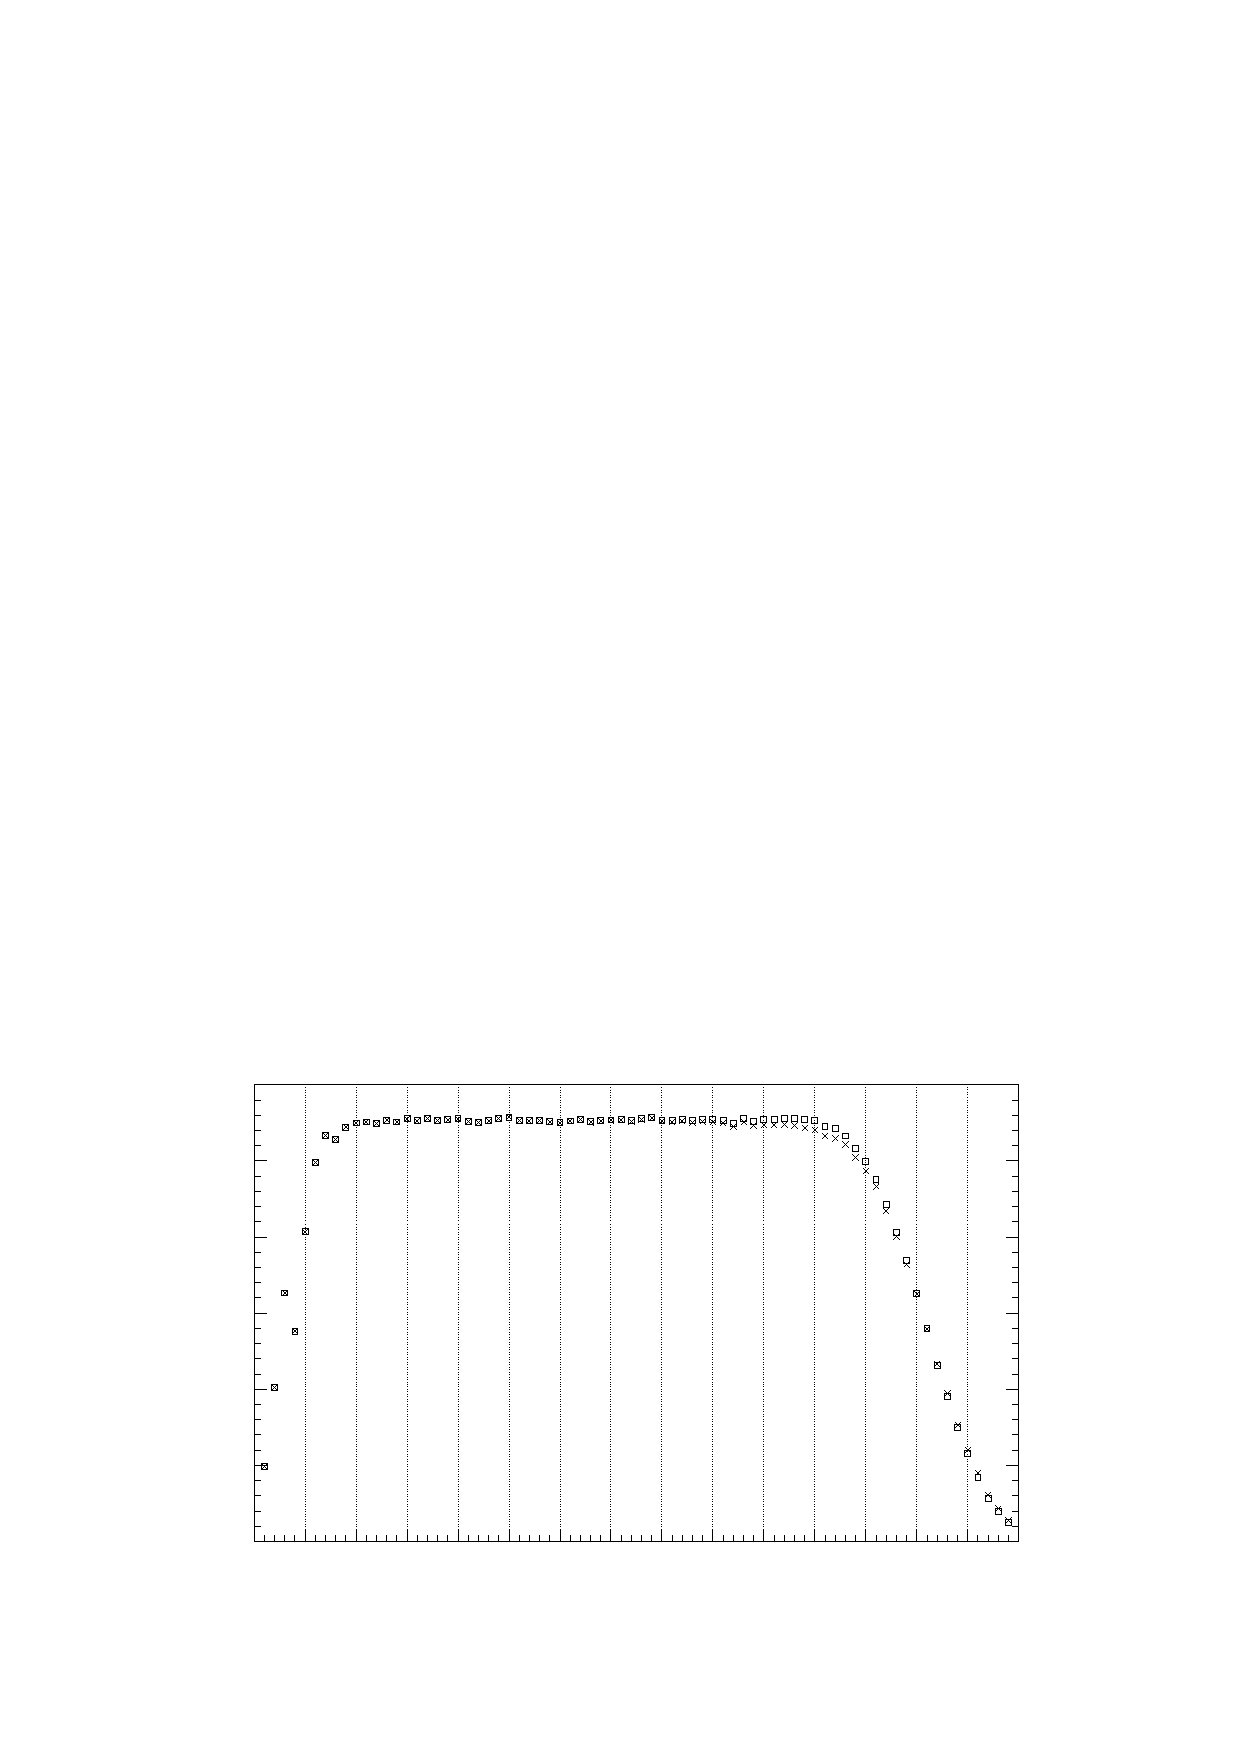
\includegraphics{reembed/sequential/bl}
\caption{\label{fig:sequential-bl_blm}
  Normalized border length per masking step of a $500\times 500$ chip before
  ({\tiny $\boxdot$}) and after ({\tiny $\times$}) a re-embedding phase with
  Sequential for border length minimization. Layout was produced by the Greedy
  placement algorithm for border length minimization with $0$-threading and
  $Q=20$K.}
\end{figure}

\begin{figure}[t]\centering
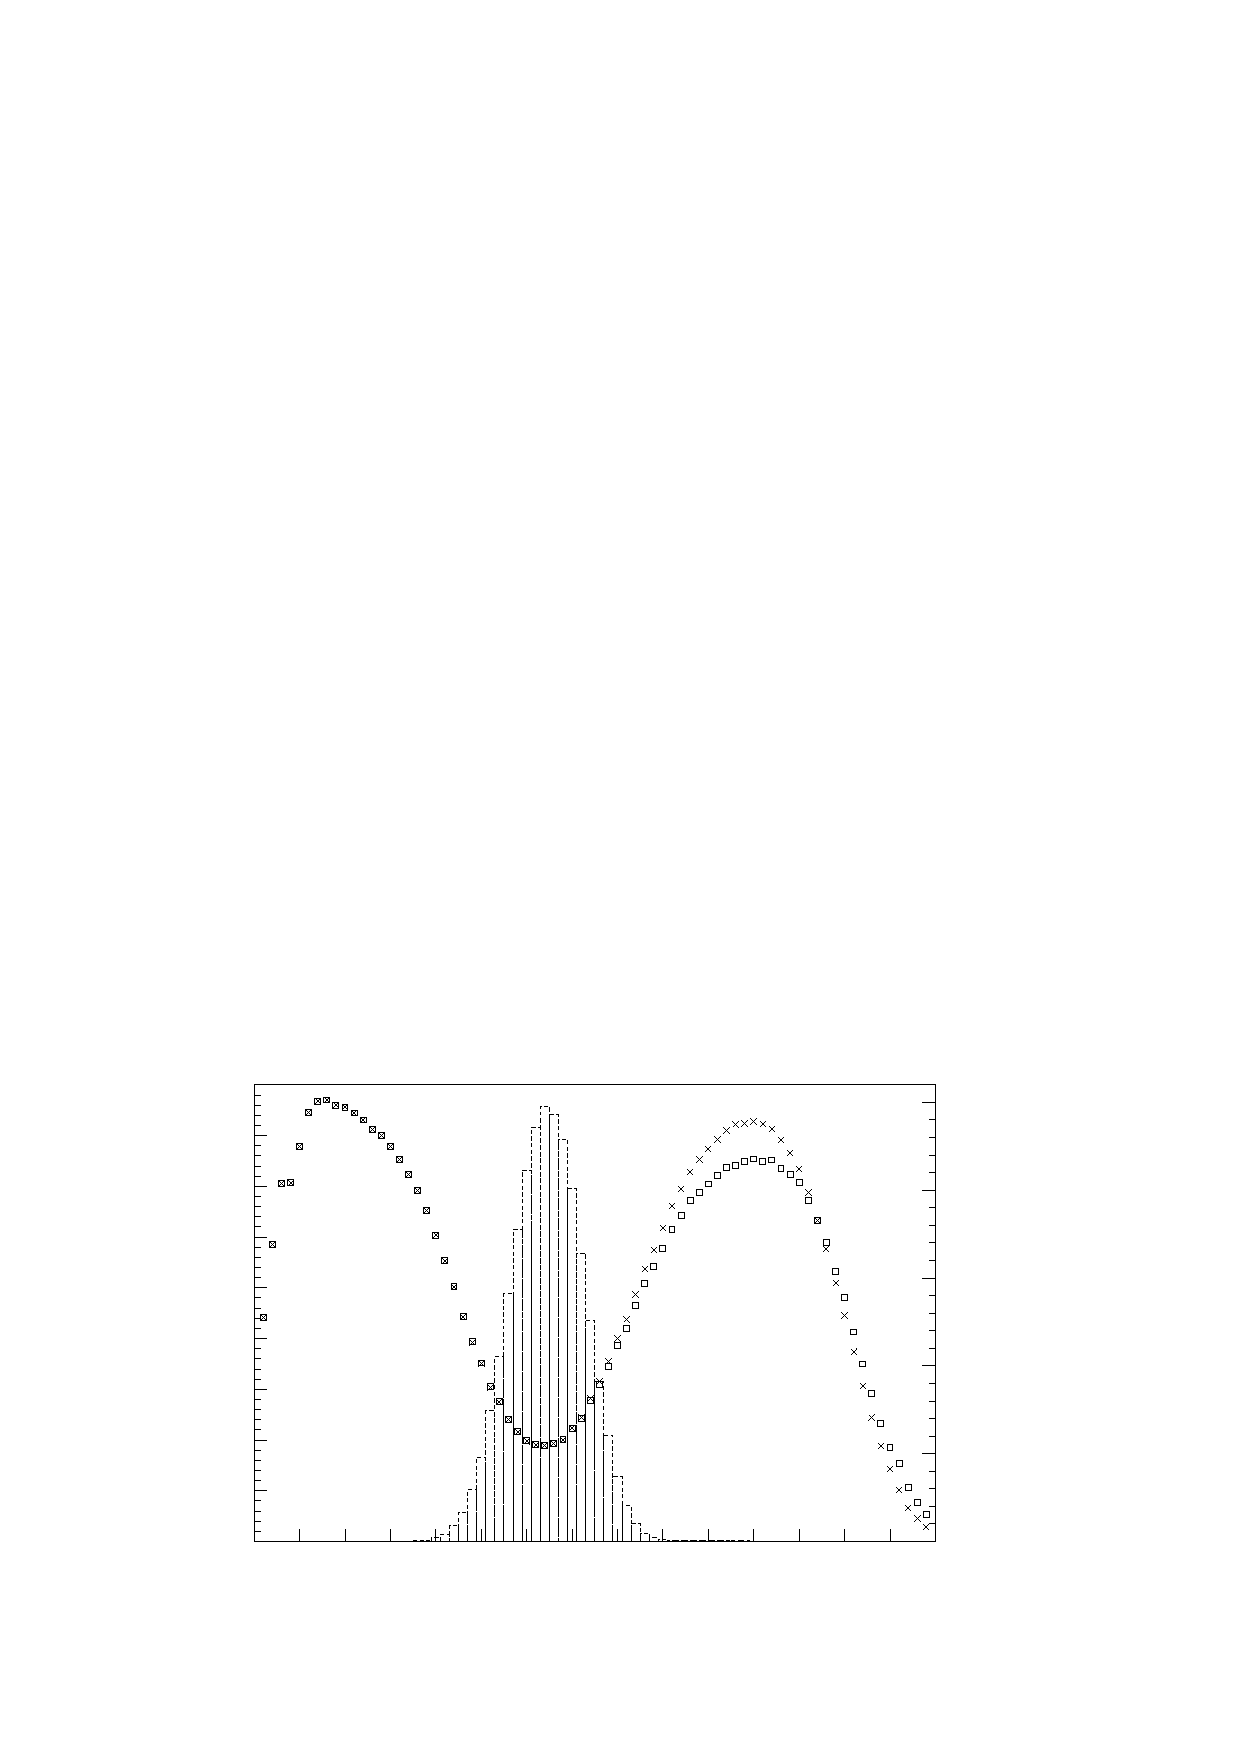
\includegraphics{reembed/sequential/ci}
\caption{\label{fig:sequential-ci_blm}
  Normalized border length per masking step of a $500\times 500$ chip before
  ({\tiny $\boxdot$}) and after ({\tiny $\times$}) a re-embedding phase with
  Sequential for conflict index minimization. Layout was produced by the Greedy
  placement algorithm for conflict index minimization with $0$-threading and
  $Q=20$K. The number of middle bases synthesized at each step is shown in boxes
  (right y-axis)}
\end{figure}

%%%%%%%%%%%%%%%%%%%%%%%%%%%%%%%%%%%%%%%%%%%%%%%%%%%%%%%%%%%%%%%%%%%%%%%%%%%%%%%%
\section{Priority re-embedding}
\label{sec:reembed_priority}

In this section we describe a new re-embedding algorithm, called Priority
re-embedding (PR), which uses a priority queue to control the order in which
probes are re-embeded.

The algorithm starts by scanning the chip for probes which have a unique
embedding in the deposition sequence. These are called \emph{pivots} and
they are used as starting locations from where the re-embeddings propagate to
other spots of the chip: Once a pivot is found, all of its four adjacent
spots on the chip are added to the priority queue. (We assume that the chip
has at least one pivot, otherwise the deposition sequence could be shortened. If
this is not the case, however, we can also use probes with the minimum number of
embeddings among all probes as pivots.)

The priority queue is used to retrieve the next spot $s$ whose probe $p$ should
be re-embedded, according to the defined priority. Once a probe $p$ is
retrieved, it is optimally re-embedded in regards to its neighbors, and all four
spots adjacent to $s$ are added to the queue (if they have not been added
previously).

We have implemented two different priorities: one based on the number of
embeddings of each probe, and one based on the number re-embedded neighbors.

\paragraph{Priority I:} Re-embed probes with fewer embeddings first.

The argument behind this priority is based on the observation that probes with
more possible embeddings have a greater degree of freedom and can more easily
``adapt'' to its neighbors. Probes with a restricted number of embeddings, on
the other hand, have less choices and should be re-embedded first.

\paragraph{Priority II:} Re-embed probes with greater number of re-embedded
neighbors first.

This priority tries to mimic the \emph{seeded crystal growth} used by the
Epitaxial placement algorithm (Section~\ref{sec:placement_epitaxial}), giving
preference to probes with a greater number of re-embedded neighbors. The
argument behind this priority is that probes should not be re-embedded until a
sufficient number of its neighbors have found their final embeddings.

With this priority, we assign a weight $w(s)$ for each spot $s$ in the queue,
and the spot with the highest weight is retrieved. In case of border length
minimization, $w(s)$ is set to the the number of immediate neighbors of $s$ that
have already been re-embedded in the current iteration.

In case of conflict index minimization, the algorithm looks at all 48 neighbors
in the $7\times 7$ region centered around $s$, and assigns a weight taking into
account the distance-dependent function $\gamma$
(Equation~\ref{eq:dist_weight}):
\[
w(s) := \sum_{\substack{s'\text{: neighbor}\\\text{of } s}}
        \Ind{s'\text{ has been re-embedded}}
        \cdot \gamma(s,s'),
\]
%%
where $s'$ ranges over all neighboring spots that are at most three cells away
(horizontally and vertically) from $s$, in accordance with the conflict index
model (Section~\ref{sec:mlp_conflict_index}).

With Priority II, once a probe is re-embedded, it is necessary to update the
weights of its neighbors that habe been previously added to the queue (up to 4
with border length minimization, and 48 with conflict index minimization).

\subsection{Results}

Tables \ref{tab:priority_bl} and \ref{tab:priority_ci} shows the results of
using Priority re-embedding on the same set of arrays used for Sequential
(Tables \ref{tab:sequential_bl} and \ref{tab:sequential_ci}). In terms of BLM,
both priorites resulted in negligible improvements when compared to Sequential
(with Priority I giving the best results). The greatest difference was only
$0.0032\%$ (from $18.2121$ with Sequential to $18.2115$ with Priority I on
$300\times 300$ chips and Greedy placement with $Q=5$K). Moreover, Priority I
was between $8.8\%$ and $12.7\%$ slower than Sequential, whereas Priority II was
between 2 to 5 times slower than Sequential.

Priority II is slower than Priority I because after it re-embeds a spot $s$, it
needs to update the weights of all neighbors of $s$ that have been previously
added to the queue. With Priority I, the nuber of embeddings of each probe does
not change, so they are computed only once, before the first iteration.

In terms of CIM, Priority I produced the worse layouts, whereas Priority II once
again achieved negligible improvements when compared to Sequential --- at most
$0.0029\%$ (from $412.5536$ to $412.5418$ on $300\times 300$ chips and Greedy
placement with $Q=20$K). The difference in running times between Sequential and
Priority dropped in comparison with the same difference in the BLM case. This is
because OSPE is significantly slower with CIM, so the extra time spent
re-embedding probes reduces the impact of the extra work with the priority
queue. For this reason, Priority I was always within $0.1\%$ of the time
required by Sequential, whereas Priority II was at most $11.37\%$ slower.

\begin{table}[t]\centering
\caption{\label{tab:priority_bl}
  Normalized border length (NBL) before and after an optimization phase with
  various re-embedding algorithms. Placement was produced by the Greedy
  placement algorithm with border length minimization, $0$-threading, and number
  $Q$ of candidates per spot set to 5K and 20K. In all cases, each re-embedding
  algorithm executed two passes before the threshold $W=0.2\%$ was reached. Best
  results are highlighted in bold.}
\footnotesize{
\begin{tabular}{crrlrrlrrlrr}
\vspace{1pt}
     & \multicolumn{2}{c}{Greedy placement} & & \multicolumn{2}{c}{Sequential} & & \multicolumn{2}{c}{Priority I} & & \multicolumn{2}{c}{Priority II} \\ \cline{2-3} \cline{5-6} \cline{8-9} \cline{11-12}
\vspace{1pt}
Dim. & $Q$ & NBL & & NBL & Time & & NBL & Time & & NBL & Time \\
\hline
$300\times 300$ &  5K & 18.3182 &  & 18.2121 &  4.8 &  & {\bf 18.2115} &  5.4 &  & 18.2118 &  22.0 \\
                & 20K & 18.0576 &  & 17.9726 &  4.8 &  & {\bf 17.9721} &  5.4 &  & 17.9723 &  14.5 \\
\hline
$500\times 500$ &  5K & 17.5830 &  & 17.4851 & 12.7 &  & {\bf 17.4848} & 13.9 &  & 17.4849 &  76.7 \\
                & 20K & 17.3554 &  & 17.2779 & 12.6 &  & {\bf 17.2776} & 13.7 &  & 17.2777 &  63.9 \\
\hline
$800\times 800$ &  5K & 16.9124 &  & 16.8201 & 32.6 &  & {\bf 16.8198} & 36.1 &  & 16.8199 & 187.0 \\
                & 20K & 16.6980 &  & 16.6258 & 32.4 &  & {\bf 16.6256} & 35.3 &  & 16.6257 & 200.0 \\
\hline
\end{tabular}}
\end{table}

\begin{table}[t]\centering
\caption{\label{tab:priority_ci}
  Average conflict index (ACI) before and after an optimization phase with
  various re-embedding algorithms. Placement was produced by the Greedy
  placement algorithm with conflict index minimization, $0$-threading, and number
  $Q$ of candidates per spot set to 5K and 20K. In all cases, each re-embedding
  algorithm executed two passes before the threshold $W=0.2\%$ was reached. Best
  results are highlighted in bold.}
\footnotesize{
\begin{tabular}{crrlrrlrrlrr}
\vspace{1pt}
     & \multicolumn{2}{c}{Greedy placement} & & \multicolumn{2}{c}{Sequential} & & \multicolumn{2}{c}{Priority I} & & \multicolumn{2}{c}{Priority II} \\ \cline{2-3} \cline{5-6} \cline{8-9} \cline{11-12}
\vspace{1pt}
Dim. & $Q$ & NBL & & NBL & Time & & NBL & Time & & NBL & Time \\
\hline
$300^2$ &  5K & 440.5166 &  & 436.8630 &  188.9 &  & 436.8881 &  190.7 &  & {\bf 436.8626} &  209.0 \\
                & 20K & 415.5003 &  & 412.5536 &  189.9 &  & 412.5613 &  190.0 &  & {\bf 412.5418} &  205.1 \\
\hline
$500^2$ &  5K & 432.3023 &  & 428.7410 &  527.3 &  & 428.7640 &  527.2 &  & {\bf 428.7375} &  581.6 \\
                & 20K & 401.4609 &  & 398.6096 &  528.3 &  & 398.6261 &  530.0 &  & {\bf 398.6065} &  569.5 \\
\hline
$800^2$ &  5K & 426.0757 &  & 422.6277 & 1357.9 &  & 422.6478 & 1357.9 &  & {\bf 422.6223} & 1512.2 \\
                & 20K & 392.1786 &  & 389.3929 & 1352.5 &  & 389.4075 & 1355.3 &  & {\bf 389.3903} & 1488.9 \\
\hline
\end{tabular}}
\end{table}

%%%%%%%%%%%%%%%%%%%%%%%%%%%%%%%%%%%%%%%%%%%%%%%%%%%%%%%%%%%%%%%%%%%%%%%%%%%%%%%%
\section{Summary}
\label{sec:reembed_summary}

In this chapter, we have presented an extension of the Optimum Single Probe
Embedding algorithm (OSPE) of \citet{Kahng2002} that is general enough to work
with border length as well as conflict index minimization. We have also surveyed
re-embeddings algorithms based on OSPE and presented experimental results with
Sequential, the best known algorithm to date.

In our results, it is evident that there is little room for improvements by
re-embedding probes once a placement is fixed. Nonetheless, we have also
introduced a new re-embedding algorithm that attempts to obtain better results
by changing the order of re-embeddings based on priorities. We have experimented
with two priorities: probes with fewer embeddings first (Priority I) and probes
with more re-embedded neighbors (Priority II).

Our results show that our algorithm can achive negligible improvements when
compared to Sequential, with Priority I being the best for BLM and Priority II
the best for CIM. However, because of the extra time required by Priority,
Sequential offers a better trade-off between solution quality and running time,
and it should still be the algorithm of choice unless when time is not
constrained. The results with our new algorithm also give further indication
that the improvements achievable in the re-embedding phase are rather small.

%%%%%%%%%%%%%%%%%%%%%%%%%%%%%%%%%%%%%%%%%%%%%%%%%%%%%%%%%%%%%%%%%%%%%%%%%%%%%%%%
\chapter{Partitioning Algorithms}
\label{ch:part}
%%%%%%%%%%%%%%%%%%%%%%%%%%%%%%%%%%%%%%%%%%%%%%%%%%%%%%%%%%%%%%%%%%%%%%%%%%%%%%%%

We mentioned earlier that the Microarray Layout Problem is usually approached in
two phases: placement and re-embedding. The placement, however, can be preceded
by a \emph{partitioning} phase that breaks the problem into smaller sub-problems
that are easier to manage. This is especially helpful for placement algorithms
with non-linear time or space complexities that are otherwise unable to handle
very large chips.

A partitioning algorithm divides the set of probes $\mathcal{P}$ into smaller
subsets, and assigns them to defined regions of the chip. Each region can then
be treated as an independent chip (and processed by a placement algorithm) or be
recursively partitioned. Linear-time placement algorithms may also benefit from
a partitioning since probes with similar embeddings are typically assigned to
the same region --- Greedy and Row-Epitaxial (Chapter~\ref{ch:placement}), for
instance, are more likely to find good candidates for filling the spots.

We describe four partitioning algorithms: 1-Dimensional Partitioning (1-DP),
2\hyph Dimensional Partitioning (2-DP), Centroid-based Quadrisection (CQ), and
Pivot Partitioning (PP). Like placement algorithms, they assume that an initial
(left-most, right-most, synchronous or otherwise pre-computed) embedding of the
probes is given. Pivot Partitioning is the only algorithm that modifies these
embeddings.  As we shall see, 1-DP and 2-DP generate a few masks with extremely
few conflicts, but leave the remaining masks with high levels of conflicts that
are difficult to handle. CQ and PP offer a more uniform optimization over all
masks. Earlier results indicate that PP produces better layouts than CQ on large
chips \citep{Carvalho2006}.

Partitioning is clearly a compromise in solution quality since it restricts the
space of solutions and may lead to conflicts at partition borders, although it
can improve solution quality when the placement algorithm cannot handle large
regions well. Hence, it is not advisable to perform too many levels of
partitioning because smaller sub-regions mean less freedom for optimization
during placement. The right balance depends on the chip dimensions as well as on
the placement and partitioning algorithms.

%%%%%%%%%%%%%%%%%%%%%%%%%%%%%%%%%%%%%%%%%%%%%%%%%%%%%%%%%%%%%%%%%%%%%%%%%%%%%%%%
\section{1-Dimensional Partitioning}
\label{sec:part_1d}

1-Dimensional Partitioning (1-DP) divides the set of probes based on the state
of their embeddings at a particular synthesis step. It starts by creating two
subsets of $\mathcal{P}$:
%%
\[
\mathcal{P}_0 = \{ p_k \in \mathcal{P} | \eps_{k,1} = 0 \},
\qquad
\mathcal{P}_1 = \{ p_k \in \mathcal{P} | \eps_{k,1} = 1 \}.
\]

In other words, $\mathcal{P}_0$ contains all probes whose embeddings are
unproductive during the first synthesis step, whereas $\mathcal{P}_1$ contains
probes with productive embeddings. The chip is then divided into two horizontal
(or vertical) bands, proportionally to the number of probes in $\mathcal{P}_0$
and $\mathcal{P}_1$, so each band accommodates one subset of $\mathcal{P}$.

This procedure is recursively applied to each band, using the the next synthesis
steps to further divide each subset of probes. For instance, the following
subsets of $\mathcal{P}_0$ and $\mathcal{P}_1$ are created during step $t=2$:
%%
\[
\mathcal{P}_{00} = \{ p_k \in \mathcal{P}_0 | \eps_{k,2} = 0 \},
\qquad
\mathcal{P}_{01} = \{ p_k \in \mathcal{P}_0 | \eps_{k,2} = 1 \},
\]
\[
\mathcal{P}_{10} = \{ p_k \in \mathcal{P}_1 | \eps_{k,2} = 0 \},
\qquad
\mathcal{P}_{11} = \{ p_k \in \mathcal{P}_1 | \eps_{k,2} = 1 \}.
\]

\begin{figure}\centering
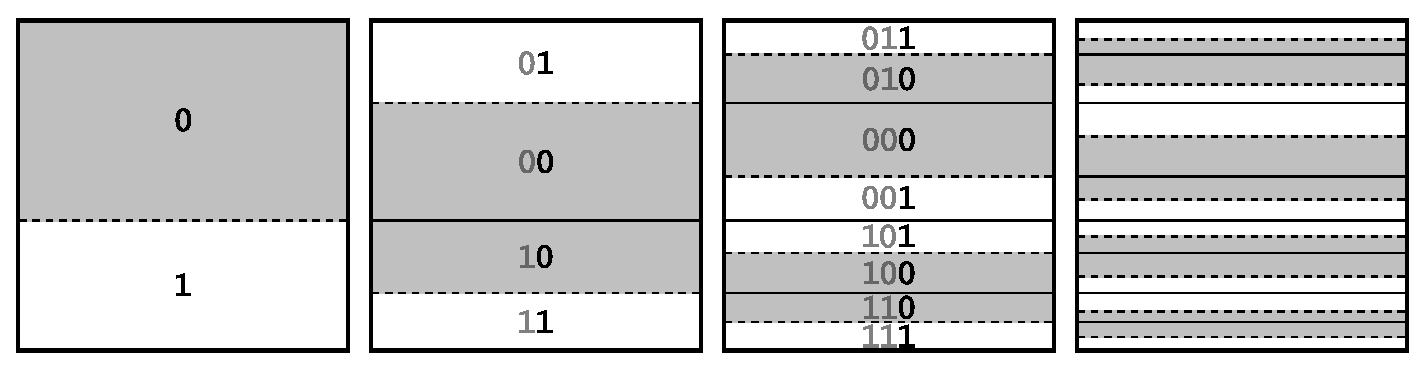
\includegraphics[width=\textwidth]{1dpart.eps}
\caption{\label{fig:1dpart}%
  First four levels of 1-Dimensional Partitioning. Dashed lines show the
  divisions performed in each step; solid lines indicate regions delimited in
  previous steps (there are no border conflicts between spots separated by
  solid lines). Masked (shaded) regions are labeled ``0'',
  unmasked (white) regions are labeled ``1''. This labeling forms
  a binary Gray code (shown in the first three steps only).}
\end{figure}

The next assignments of subsets to the upper or lower band of their regions are
made in such a way that regions with the same ``state'' --- productive
(unmasked) or unproductive (masked) --- are joined as far as possible, resulting
in masks that consist of alternating layers of masked and unmasked spots. This
process is illustrated in Figure~\ref{fig:1dpart}, where at each step~$t$, a
band is labeled ``0'' when its embeddings are unproductive, and ``1'' when its
embeddings are productive. The resulting binary numbers from top to bottom form
a binary Gray code, that is, a permutation of the binary numbers between 0 and
$2^n - 1$ such that neighboring elements have exactly one differing bit, as do
the first and last elements \citep{Kreher1999}.

The Gray code highlights an interesting property of 1-DP. After $d$~levels of
partitionings (based on steps $1$ to $d$), the embeddings of any two immediate
neighbors differ among the first $d$~steps in at most one step.  As a result,
masks $M_1 \dots M_d$ exhibit a layered structure that effectively reduces
border conflicts.

Unfortunately, the Gray code is disrupted as soon as a region cannot be divided
(because all probes of that region are, for instance, masked at a particular
step). This will certainly happen as several binary numbers are unlikely to be
substrings of embeddings (think of, for example, a long run of zeros).

Moreover, 1-DP can optimize only a limited number of masks because the
sub-regions soon become too narrow to be further divided. The maximum
\emph{partitioning depth} $d_{max}$ is primarily limited by the number of rows
(or columns) on the chip. In practice, since regions are likely to be unevenly
divided, $d_{max}$ varies between regions. The algorithm can also be configured
to stop partitioning a region once its height drop below a given threshold
$H_{max}$ (i.e., the maximum height of any final region will not exceed
$H_{max}$).

1-DP is easier to implement if the partitionings always produce rectangular
regions (i.e., splitting a row between two regions is not allowed). In order to
force an exact division of a region, however, it might be necessary to move a
few probes from one subset of probes to the other one.

For example, imagine that a chip with $|\mathcal{P}| = 900$ probes, $n_r = 30$
rows and $n_c = 30$ columns is to be partitioned based on the state of the
embeddings at the first synthesis step, resulting in sub-sets $\mathcal{P}_0$
and $\mathcal{P}_1$ with, say, 638 and 262 probes, respectively. The chip must
thus be divided into two sub-regions, the upper one containing
$[30 \cdot 638/900]=21$ rows and the lower one with $[30 \cdot 262/900]=9$ rows
($[x]$ is $x$ rounded to the nearest integer). The problem is that the upper
region then contains $21 \cdot 30 = 630$ spots but it has to accommodate 638
probes, whereas the lower region contains $9 \cdot 30 = 270$ spots but only 262
probes. The solution is to (arbitrarily) move 8 probes from $\mathcal{P}_0$ to
$\mathcal{P}_1$, which, results in some imperfections in the layers of the
corresponding mask (a few masked spots in a region of unmasked spots and
vice-versa).

%%%%%%%%%%%%%%%%%%%%%%%%%%%%%%%%%%%%%%%%%%%%%%%%%%%%%%%%%%%%%%%%%%%%%%%%%%%%%%%%
\section{2-Dimensional Partitioning}
\label{sec:part_2d}

\begin{figure}[t]\centering
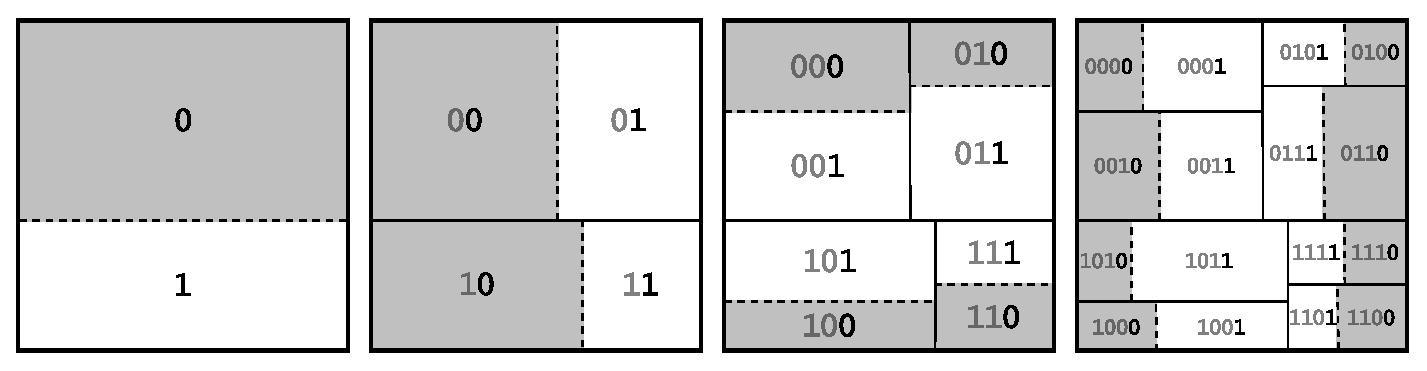
\includegraphics[width=\textwidth]{2dpart.eps}
\caption{\label{fig:2dpart}%
  First four levels of 2-Dimensional Partitioning. Dashed lines show the
  divisions performed in each step; solid lines indicate regions delimited in
  previous steps. Masked regions are labeled with ``0'', unmasked regions with
  ``1''; this labeling forms an approximation to a two-dimensional binary Gray
  code.}%
\end{figure}

The 2-Dimensional Partitioning algorithm extends the idea of 1-DP to two
dimensions, with the potential of optimizing twice as many masks. The algorithm
is similar: $\mathcal{P}$ is divided into subsets based on the state of the
embeddings at a particular synthesis step. The differences are that 2-DP
alternates horizontal and vertical divisions of regions, and that the
assignments of probes to regions obey a two-dimensional binary Gray code (Figure
\ref{fig:2dpart}). In a 2-D Gray code, the binary numbers are arranged in a
matrix in such a way that two neighboring numbers differ in at most one bit. As
a result, regions whose embeddings are at the same state (productive or
unproductive) are joined as far as possible.

If regions were always equally divided, 2-DP would have the same property as 1-
DP: After $d$~levels of partitionings (based on steps $1$ to $d$), the
embeddings of any two immediate neighbors would differ among the first $d$ steps
in at most one step. However, this is not always the case since 2-DP is likely
to create regions with different dimensions, forcing some regions to share a
border with more than its four natural neighbors. For instance, in
Figure~\ref{fig:2dpart} region ``0010'' borders with ``0000'', ``1010'', and
``0011'', but also with ``0001'' and ``1011''.

Like 1-DP, the maximum partitioning depth, $d_{max}$, is limited by the number
of rows and columns on the chip, and it varies since regions are likely to be
unevenly divided. 2-DP can also be configured to stop partitioning a region once
its dimensions (height and width) drop bellow a given threshold $L_{max}$ (the
largest final region will contain at most ${L_{max}}^2$ spots).

Figure \ref{fig:2dpart_bl} shows the normalized border length per masking step
of layouts produced by 2-DP for a $1\,000\times 1\,000$ chip. With maximum
partitioning depth ($L_{max}=1$), 2-DP produced a layout with the best masks for
the first 22 synthesis steps. However, because the chip is partitioned until all
regions are $1\times 1$ (containing a single probe), the placement algorithm has
no freedom for reducing border conflicts in the remaining masks. As a result,
from step 33 on, the levels of border conflicts are as high as in the random
layout.

With $L_{max}=10$, there is more room for optimization during placement since
the final regions can be as large as $10\times 10$. In this case, we used the
Greedy placement algorithm (Section~\ref{sec:placement_greedy}) with $Q=100$ so
that all probes of a region were considered for filling its spots. This resulted
in a reduction of about $13.4\%$ in normalized border length compared to the
layout produced with $L_{max}=1$ (from $21.5588$ to $18.6670$, data not shown),
although we observed an increase of border conflicts in the first 24 masks.
Increasing $L_{max}$ even further to 50 and using Greedy with $Q=2\,500$
resulted in a reduction of $8.1\%$ in normalized border length compared to
$L_{max}=10$ (from $18.6670$ to $17.1629$) but, again, this came at the expense
of an increase of border conflicts in the first 20 masks.

\begin{figure}[t]\centering
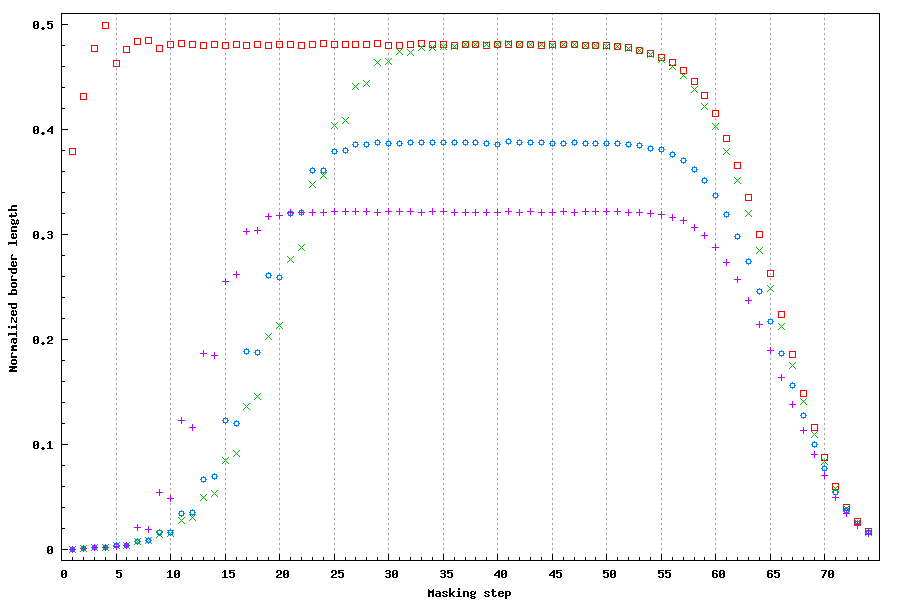
\includegraphics{part/2dpart/bl}
\caption{\label{fig:2dpart_bl}
  Normalized border length per masking step of several layouts for a
  $1\,000\times 1\,000$ chip with random probes left-most embedded in the
  standard Affymetrix depostion sequence: random layout ({\tiny $\boxdot$}); 2-D
  Partitioning with $L_{max}=1$ ({\scriptsize $\times$}); 2-D Partitioning with
  $L_{max}=10$ and Greedy placement with $Q=100$ ({\tiny $\odot$}); 2-D
  Partitioning with $L_{max}=50$ and Greedy placement with $Q=2\,500$
  ({\tiny $+$}).}
\end{figure}

Figure~\ref{fig:1dp_versus_2dp} compares the results obtained by 1-DP and 2-DP
on the same $1\,000\times 1\,000$ chip of Figure \ref{fig:2dpart_bl}. We first
compare both algorithms with their maximum partitioning depths ($H_{max}=1$ for
1-DP and $L_{max}=1$ for 2-DP). With $L_{max}=1$, 2-DP produces $1\times 1$
regions and leaves no room for optimization during placement. In constrast, 1-DP
with $H_{max}=1$ produces regions with a single row but, in this case, with
$1\,000$ columns (and $1\,000$ probes), leaving a considerable degree of
flexibility for the placement algorithm. To be fair, we thus compare 1-DP and
2-DP using a placement algorithm that places probes randomly inside each final
region, so that the results are only due to the partitionings (and not to the
placement algorithm). In our results, with maximum partitioning depths, 1-DP and
2-DP produced layouts with similar levels of border conflicts in mask
$M_{33} \dots M_{74}$, although the layout produced by 2-DP was slightly better
in masks $M_{58} \dots M_{69}$. However, while 1-DP was able to produce masks
with relatively few conflicts in the first 17 steps, 2-DP achieved even greater
reductions of border conflicts in the first 32 steps. The normalized border
length of these layouts are $25.8543$ (with 1-DP) and $21.5588$ (with 2-DP).

In Figure~\ref{fig:1dp_versus_2dp} we also compare 1-DP with $H_{max}=1$ and
2-DP with $L_{max}=50$ using Greedy for the placement. With $L_{max}=50$, 2-DP
produces regions containing at most $2\,500$ probes. For this particular chip,
2-DP produced $1\,005$ regions, containing $995.02$ probes on average (the
largest region contained $2\,209$ and the smallest $210$ probes), so Greedy had
about the same degree of freedom provided by 1-DP with $H_{max}=1$. We used a
sufficiently large number $Q$ of candidates per spot so that all probes of a
region were considered for filling its spots. With these settings, the layouts
produced by 1-DP and 2-DP have similar levels of border conflicts in masks
$M_{20} \dots M_{74}$. In the first 18 synthesis steps, however, 2-DP produced
better masks, especially after step 5. The normalized border length of these
layouts are $18.0078$ (1-DP) and $17.1629$ (2-DP).

\begin{figure}[t]\centering
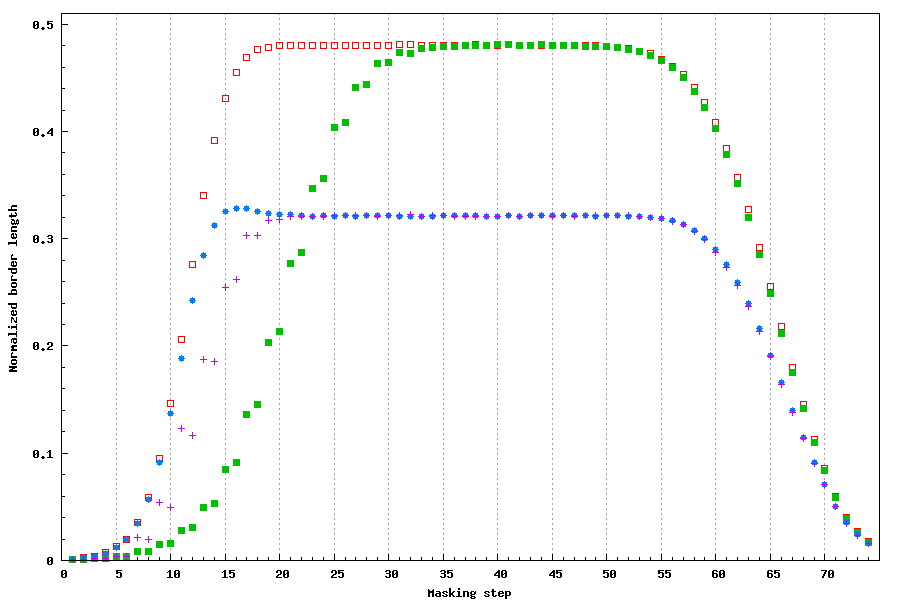
\includegraphics{part/1d_versus_2d/bl}
\caption{\label{fig:1dp_versus_2dp}
  Normalized border length per masking step of layouts produced by 1-D and 2-D
  Partitioning for a $1\,000\times 1\,000$ chip with random probes left-most
  embedded in the standard Affymetrix depostion sequence: 1-DP with $H_{max}=1$
  and random placement ({\scriptsize $\times$}); 2-DP with $L_{max}=1$
  ({\tiny $\boxdot$}); 1-DP with $L_{max}=1$ and Greedy placement with $Q=1$K
  ({\tiny $+$}); 2-DP with $L_{max}=50$ and Greedy placement with $Q=2.5$K
  ({\tiny $\odot$}) .}
\end{figure}

A representation of selected photolithographic masks generated by 2-DP for a
$300\times 300$ chip are shown in Figure \ref{fig:2dpart_masks}. The resulting
rectangular regions can be seen, clearly, up to mask $M_{18}$. In the first
eight masks it is possible to see some ``imperfections'' (unmasked spots on
masked regions or vice-versa) that result from arbitrarily moving probes between
regions in order to force exact divisions. On a chip of this size, 2-DP can
usually reduce conflicts up to the $25^{\mathrm{th}}$ synthesis step, although
this is not noticeable in $M_{25}$ of Figure \ref{fig:2dpart_masks}.

\begin{figure}[p]\centering
%%
\begin{picture}(435,567)\footnotesize{
\put( -2,439){\makebox(145,128){
\includegraphics{part/2dmasks/mask01}}}
\put(147,439){\makebox(145,128){
\includegraphics{part/2dmasks/mask02}}}
\put(292,439){\makebox(145,128){
\includegraphics{part/2dmasks/mask03}}}
\put( -2,429){\makebox(145, 10){$M_1$}}
\put(147,429){\makebox(145, 10){$M_2$}}
\put(292,429){\makebox(145, 10){$M_3$}}
\put( -2,296){\makebox(145,128){
\includegraphics{part/2dmasks/mask04}}}
\put(147,296){\makebox(145,128){
\includegraphics{part/2dmasks/mask05}}}
\put(292,296){\makebox(145,128){
\includegraphics{part/2dmasks/mask06}}}
\put( -2,286){\makebox(145, 10){$M_4$}}
\put(147,286){\makebox(145, 10){$M_5$}}
\put(292,286){\makebox(145, 10){$M_6$}}
\put( -2,153){\makebox(145,128){
\includegraphics{part/2dmasks/mask07}}}
\put(147,153){\makebox(145,128){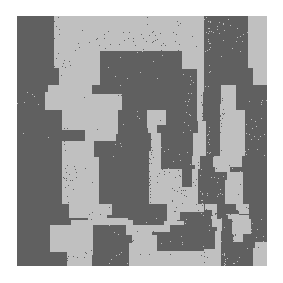
\includegraphics{part/2dmasks/mask08}}}
\put(292,153){\makebox(145,128){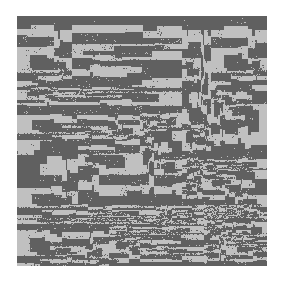
\includegraphics{part/2dmasks/mask13}}}
\put( -2,143){\makebox(145, 10){$M_7$}}
\put(147,143){\makebox(145, 10){$M_8$}}
\put(292,143){\makebox(145, 10){$M_{13}$}}
\put( -2, 10){\makebox(145,128){
\includegraphics{part/2dmasks/mask18}}}
\put(147, 10){\makebox(145,128){
\includegraphics{part/2dmasks/mask25}}}
\put(292, 10){\makebox(145,128){
\includegraphics{part/2dmasks/mask68}}}
\put( -2,  0){\makebox(145, 10){$M_{18}$}}
\put(147,  0){\makebox(145, 10){$M_{25}$}}
\put(292,  0){\makebox(145, 10){$M_{68}$}}
}\end{picture}
%%
\caption{\label{fig:2dpart_masks}%
  Selected masks generated by 2-Dimensional Partitioning with $L_{max}=1$ for a
  random $300\times 300$ chip with 25-mer probes leftmost embedded into the
  standard Affymetrix deposition sequence. Unmasked (masked) spots are
  represented by light (dark) dots.}
\end{figure}

So far we have described both 1-DP and 2-DP using the state of the first $d$
synthesis steps to divide the set of probes. The result of this approach is
that, while the first masks are optimized, the remaining masks are left with
high levels of border conflicts; we call this a \emph{left-most mask
optimization}.

However, a defect in the middle of the probe is more harmful than in its
extremities, so it is more important to optimize the central masks that are more
likely to synthesize the probes' middle bases. Fortunately, it is possible to
reduce conflicts in the central masks using 1-DP and 2-DP by partitioning the
probe set based on the following sequence of synthesis steps, assuming that $T$
is even and $d$ is odd:
$T/2, (T/2)\pm 1, (T/2)\pm 2, \dots, (T/2)\pm\lfloor d/2\rfloor$; we call this a
\emph{centered mask optimization}.

\begin{figure}[t]\centering
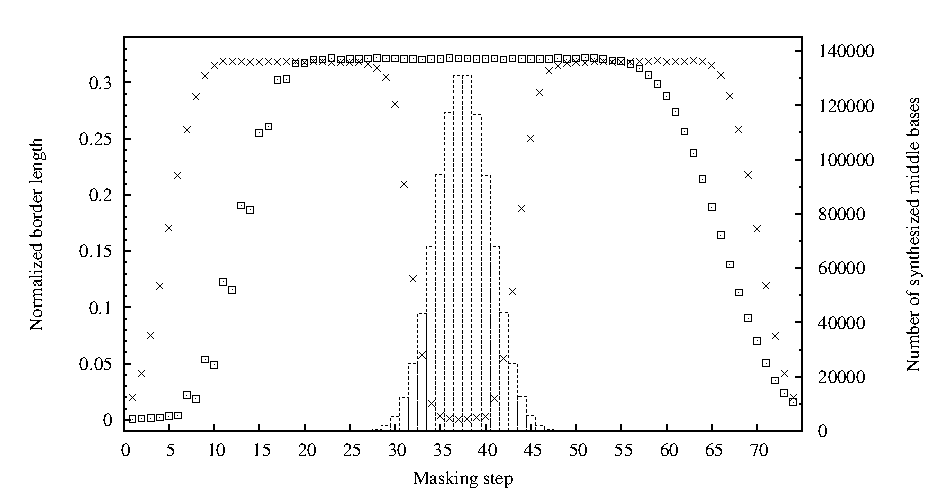
\includegraphics{part/left_versus_central/bl}
\caption{\label{fig:2d_left_center}
  Normalized border length per masking step (on the left y-axis) of two layouts
  produced by 2-Dimensional Partitioning with $L_{max}=50$ and Greedy placement
  with border length minimization and $Q=2.5$K for a $1\,000 \times 1\,000$ chip
  with random probe sequences: left-most mask optimization with left-most
  embeddings ({\tiny $\boxdot$}); centered mask optimization with centered
  embeddings ({\scriptsize $\times$}). The number of middle bases synthesized at
  each step (with centered embeddings) is shown in boxes (right y-axis).}
\end{figure}

For left-most optimization, it makes sense to embed the probes in a left-most
fashion in order to reduce conflicts in the last masks (which are not optimized
by the partitioning). The left-most embeddings reduce the number of unmasked
spots in the last steps, resulting in masks that largely consist of masked
spots and consequently low levels of border conflicts. In contrast, centered
mask optimization produces better results with \emph{centered} embeddings. A
centered embedding is constructed by shifting a left-most embedding to the right
until the number of masked steps to the left of the first productive step is
approximately equal to the number of masked steps to the right of the last
productive step.

\ignore{An aligned
embedding is constructed by shifting a left-most embedding in such a
way that the probe's middle base is synthesized during the middle cylce (or as
close as possible to it).
}%% aligned embeddings are giving worse results than centered embeddings

Figure~\ref{fig:2d_left_center} shows the results of using 2-D Partitioning with
$L_{max}=50$ on a $1\,000\times 1\,000$ chip with left-most and centered mask
optimization. With left-most mask optimization, we obtain a normalized border
length of $17.1629$ (up to approximately $0.32$ per step). With centered mask
optimization, the normalized border length improves by $1.03\%$ to $16.9855$
(not shown in the figure). The average conflict index, however, is reduced by as
much as $34.89\%$ (from $577.3353$ to $375.9232$) because of the higher weight
of the middle bases in the conflict index measure.

\begin{table}[t!]\centering
\caption{\label{tab:2dp_greedy}
  Average conflict index (ACI) of layouts produced by Greedy placement and 2-D
  Partitioning on random $800\times 800$ chips with left-most and centered
  embeddings. 2-DP was configured for centered mask optimization and used Greedy
  for the placement. In all cases, Greedy was configured for conflict index
  minimization and used $0$-threading. Results are averages over a set of five
  arrays and running times are reported in minutes.}
\footnotesize{
\begin{tabular}{clrr}
Embeddings & Algorithm & ACI & Time \\
\hline
Leftmost   & Greedy with $Q=20$K & 392.1786 & 186.4 \\
Leftmost   & Greedy with $Q=40$K & 378.3110 & 357.0 \\
Leftmost   & Greedy with $Q=80$K & 366.8446 & 680.9 \\
\hline
Centered   & Greedy with $Q=20$K & 387.5974 & 205.1 \\
\hline
Centered   & 2-DP with $L_{max}=10$ and Greedy with $Q=100$    &      345.9908  & 0.6 \\
Centered   & 2-DP with $L_{max}=20$ and Greedy with $Q=400$    &      342.2031  & 1.3 \\
Centered   & 2-DP with $L_{max}=30$ and Greedy with $Q=900$    & {\bf 341.2786} & 2.3 \\
Centered   & 2-DP with $L_{max}=40$ and Greedy with $Q=1\,200$ &      341.6185  & 4.0 \\
Centered   & 2-DP with $L_{max}=50$ and Greedy with $Q=2\,000$ &      341.7515  & 6.1 \\
Centered   & 2-DP with $L_{max}=60$ and Greedy with $Q=3\,600$ &      341.8634  & 8.4 \\
\hline
\end{tabular}}
\end{table}

%% data removed from table {tab:2dp_greedy}
%% Centered   & 2-DP with $L_{max}=25$ and Greedy with $Q=625$    &      341.4105  & 1.8 \\
%% Centered   & 2-DP with $L_{max}=35$ and Greedy with $Q=1\,225$ & {\bf 341.2372} & 2.7 \\

When carefully used, 1-DP and 2-DP can improve placement by producing a few
masks with very low levels of border conflicts and breaking the problem into
smaller sub-problems that are easier to handle. Table \ref{tab:2dp_greedy} shows
results on $800\times 800$ arrays using 2-DP with centered mask optimization and
Greedy with conflict index minimization for the placement, in comparison to
using Greedy alone (results with Greedy as shown on Table \ref{tab:greedy} and
Figure \ref{fig:greedy_tradeoff}). Results of Greedy with centered embeddings
are also shown. In our results, the layouts produced by 2-DP are even better
than the ones produced by Greedy with $Q=80$K. This is a consequence of the
importance of the middle bases in the conflict index measure. Moreover, while
Greedy required about $680.9$ minutes with $Q=80$K, the combination of 2-DP and
Greedy required at most $8.4$ minutes because the partitioning restricts the
number of candidates Greedy can look at for each spot.

Increasing $L_{max}$ provides more room for optimization during placement but
worsens the central masks, while reducing $L_{max}$ improves the central masks
at the expense of an increase of conflicts in the remaining masks (in this case,
reducing $L_{max}$ also improves running time as Greedy has fewer candidates
available for each spot). The best trade-off depends on several aspects of the
problem such as chip dimension, probe embeddings, type of optimization (border
length or conflict index), and placement algorithm. For this case, the best
results were achieved with $L_{max}=30$.

%%%%%%%%%%%%%%%%%%%%%%%%%%%%%%%%%%%%%%%%%%%%%%%%%%%%%%%%%%%%%%%%%%%%%%%%%%%%%%%%
\section{Centroid-based Quadrisection}
\label{sec:part_cq}

\begin{figure}\centering
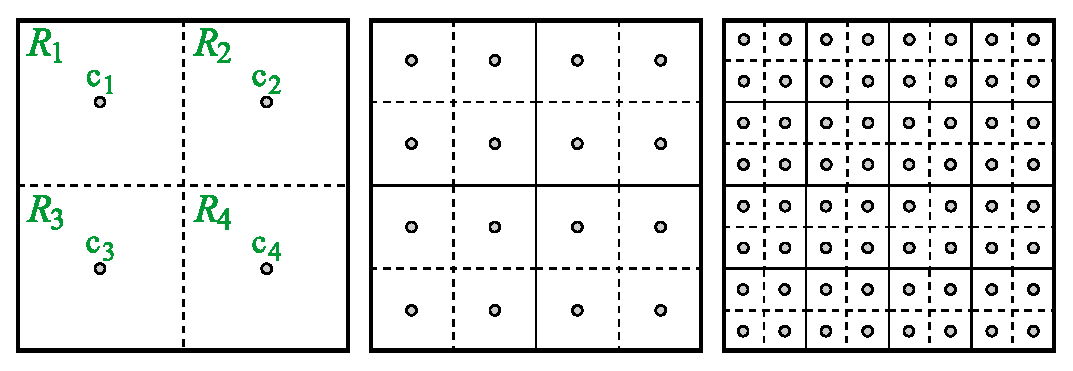
\includegraphics[width=\textwidth]{quadrisect.eps}
\caption{\label{fig:quadrisect}%
  First three levels of Centroid-based Quadrisection. Dashed lines show the
  divisions performed in each step; solid lines indicate regions delimited in
  previous steps. The centroids of each partition $R_{c_1} \dots R_{c_4}$ are
  represented by small circles (labeled with $p_{c_1} \dots p_{c_4}$ in the
  first step).}
\end{figure}

Centroid-based Quadrisection \citep{Kahng2003a}, CQ for short, employs a
different criterion for dividing the probe set and a different approach for
partitioning. At each iteration, a region $R$ is quadrisectioned into $R_{c_1}$,
$R_{c_2}$, $R_{c_3}$, and $R_{c_4}$. Each sub-region $R_{c_i}$ is associated
with a selected probe $p_{c_i}\in \mathcal{P}$, called \emph{centroid}, that is
used to guide the assignment of the remaining probes to the sub-regions.

A centroid is a representative of its region: It should symbolize the ``average
embedding'' in that region. The remaining probes
$p_k \in \CalP \setminus \{p_{c_1},p_{c_2},p_{c_3},p_{c_4}\}$ are compared to
each centroid and assigned to the sub-region $R_{c_i}$ whose centroid's
embedding $\eps_{c_i}$ has minimum $H(k,c_i)$, where $H(k,k')$ is the Hamming
distance between the embeddings $\eps_k$ of $p_k$ and $\eps_{k'}$ of $p_{k'}$
(see Section \ref{sec:mlp_border_length}).

The authors argue that, in order to improve the ``clustering'' of similar
probes, the four centroids should be as different from each other as possible.
The following heuristic is proposed: First, a probe index $c_1$ is randomly
selected from $\{1,\dots,|\mathcal{P}|\}$.  Then, a probe index $c_2\neq c_1$
maximizing $H(c_2,c_1)$ is selected.  Similarly, $c_3$ maximizing
$H(c_3,c_1) + H(c_3,c_2)$ and $c_4$ maximizing
$H(c_4,c_1) + H(c_4,c_2) + H(c_4,c_3)$ are selected.  The assignment of
centroids to the quadrisections of the chip is arbitrary.

Since the partitioning must always produce four regions of the same size,
sometimes it is necessary to make non-optimal assignment of probes to regions.
In order to recover from a possibly bad choice of centroids, a ``multi-start
heuristic'' is used, running the centroid selection procedure several times with
different ``seeds'' for $c_1$ and keeping the centroids that lead to the best
partitioning. For measuring partitioning quality, the algorithm uses the sum of
Hamming distances between the embeddings of the probes and the embedding of the
centroid (the partitioning that results in the least sum is selected).

The maximum partitioning depth $d_{max}$ of CQ is $\sqrt{n_r}$, assuming that
$n_r$ is square and that $n_c=n_r$ ($n_r$ and $n_c$ are the number of rows and
columns on the chip, respectively). In practice, the partitioning continues
until a pre-defined depth $D$ has been reached.

CQ was developed for border length minimization (BLM), but it can be adapted for
conflict index minimization (CIM) by using the \emph{conflict index distance}
$C(k,k')$ between the embeddings $\eps_k$ and $\eps_{k'}$ (as defined in Section
\ref{sec:mlp_conflict_index}) instead of the Hamming distance $H(k,k')$ for
selecting the centroids as well as for deciding which partition a probe should
be assigned to.

As mentined in Section \ref{sec:placement_greedy}, placement algorithms such as
Row-Epitaxial and Greedy have the drawback of treating the last $Q - 1$ filled
spots unfairly since fewer than $Q$ probe candidates are available to fill them.
This issue is aggravated by a partitioning because in each final partition
$Q - 1$ spots have fewer than $Q$ probe candidates. In order to attenuate this
problem, a \emph{borrowing heuristic} was implemented in CQ to allow the
placement algorithm (Row-Epitaxial, in the original implementation) to look at
$Q$ probes ``in the current and the next region''. Although the authors did not
specify the exact meaning of ``next region'', it can be, for instance, the next
region to be processed by the placement algorithm. Borrowing probes from a
region $R_{c_i}$ to fill spots of $R_{c_j}$ obviously requires using the
unplaced probes of $R_{c_j}$ to fill spots of $R_{c_i}$.

%%%%%%%%%%%%%%%%%%%%%%%%%%%%%%%%%%%%%%%%%%%%%%%%%%%%%%%%%%%%%%%%%%%%%%%%%%%%%%%%
\section{Pivot Partitioning}
\label{sec:part_pp}

Pivot Partitioning \citep{Carvalho2006}, PP for short, is to a certain extent
similar to CQ: Sub-regions are recursively associated with special probes, here
called \emph{pivots} instead of centroids, that are used to guide the assignment
of the other probes to the sub-regions. The main differences between PP and CQ
are as follows.

Instead of quadrisectioning the chip, PP creates sub-regions by alternating
horizontal and vertical divisions (like 2-D Partitioning). At each iteration, a
region $R$ is partitioned into sub-regions $R_{c_1}$ and $R_{c_2}$ associated
with pivots $q_{c_1}$ and $q_{c_2}$, respectively. The advantage of alternating
horizontal and vertical divisions over the quadrisectioning approach of CQ is
that regions are not required to have the same size. Instead, regions are
divided proportionally to the size of each subset of probes, which reduces the
need for making non-optimal assignments, although it may still be necessary to
move some probes from one sub-region to the other in order to obtain rectangular
regions. Moreover, for each partitioning, only two pivots need to be selected.

Another distinction is motivated by the same observation that inspired the
development of the Priority re-embedding algorithm (Section
\ref{sec:reembed_priority}), i.e., that different probes have different numbers
of embeddings, ranging from a single one to several millions on a typical
Affymetrix GeneChip array. Probes with more embeddings can more easily adapt to
the other probes, that is, they are more likely to have an embedding with fewer
conflicts to fill a particular spot than a probe that has only a limited number
of embeddings. PP uses probes with a single embedding (or few embeddings) as
pivots, and chooses the other probes' embeddings and region assignments
accordingly. Indeed, the most important feature of PP is the simultaneous
embedding and assignment of probes to sub-regions.

\begin{algorithm}[t!]
\caption{PivotPartitioning}
\label{alg:pp_pivots}
\begin{minipage}{\textwidth}\footnotesize{
%%
\begin{tabbing}
Output: \= \kill
Input:  \> rectangular region R consisting of all rows and columns of the chip, \\
        \> set of probes $\CalP = \{p_{1}, p_{2}, \dots p_{n}\}$, \\
        \> deposition sequence $N$, \\
        \> and maximum partitioning depth $D$ \\
Output: \> set of assignments $\CalA = \{a_1, a_2, \dots a_{2^D}\}$ \\
        \> where $a_i = (\CalP_i, R_i)$, $\CalP_i \subset \CalP$,
           and $R_i$ is a sub-region of the chip
\end{tabbing}
%%
\begin{enumerate}
\item (Select pivot candidates.) Select probes $p \in \CalP$ with minimum number
      of embeddings $E(p)$ as pivot candidates:
  \begin{enumerate}
    \item Let $\CalQ = \{p \in \CalP \;|\; E(p,N) \mbox{ is minimal}\}$
    \item Set $\CalP \leftarrow \CalP \setminus \CalQ$
  \end{enumerate}
\item (Call RecursivePartitioning.) Call recursive procedure with initial
      partitioning depth 1 and return:
  \begin{enumerate}
    \item Return RecursivePartitioning $(1, D, R, \CalQ, \CalP)$
  \end{enumerate}
\end{enumerate}
}\end{minipage}
\end{algorithm}

The first part of the algorithm consists of selecting a sub-set of probes that
will be used as pivots (Algorithm \ref{alg:pp_pivots}). First, it examines each
probe $p \in \CalP$ and computes $E(p,N)$, the number of embeddings of $p$ in
the deposition sequence $N$; this can be done in $O(\ell \cdot T)$ time with
dynamic programming, where $\ell$ is the length of the probe and $T$ is the
length of the deposition sequence. The set of pivot candidates $\CalQ$ then
consists of all probes $p$ with $E(p,N)=1$. In practice, this usually results in
a sufficient number of pivots. For instance, around $6\%$ of the probes in a
randomly generated chip have a single embedding. If this is not the case, we can
set a threshold $e$ for the maximum number of embeddings of a pivot in such a
way that the number of probes $p$ with $E(p,N)\leq e$ is at least $2^D$.

Using probes with fewer embeddings as pivots has two advantages. First, less
time is spent choosing the pivots in each iteration since fewer candidates need
to be examined. Second, probes with fewer embeddings are usually better
``representatives'' to drive the partitioning. The problem is that some
embeddings may have their productive steps concentrated in one part of the
deposition sequence. For instance, some Affymetrix probes, when left-most
embedded, are synthesized in the first 37 masking steps, thus using only half of
the total 74 steps. Such probes are not good choices for pivots. In our
experience, probes with fewer embeddings are better pivots because they cover
most (if not all) cycles of the deposition sequence.

\begin{algorithm}[t!]
\caption{RecursivePartitioning with conflict index minimization}
\label{alg:pp_recurse}
\begin{minipage}{\textwidth}\footnotesize{
%%
\begin{tabbing}
Output: \= \kill
Input:  \> current partitioning depth $d$, \\
        \> maximum partitioning depth $D$, \\
        \> rectangular region $R$ of the chip, \\
        \> set of pivot candidates $\CalQ$, \\
        \> and set of probes $\CalP$, \\
Output: \> set of assignments $\CalA = \{a_1, a_2, \dots a_{2^{(D-d)}}\}$ \\
        \> where $a_i = (\CalP_i \cup \CalQ_i, R_i)$, $\CalP_i \subset \CalP$,
           $\CalQ_i \subset \CalQ$, and $R_i$ is a sub-region of $R$
\end{tabbing}
%%
\begin{enumerate}
\item \label{step:pp_stop} (Stopping condition.) When $d = D$:
  \begin{enumerate}
    \item Re-embed each $p \in \mathcal{P}$ optimally with respect to all
          $q \in \mathcal{Q}$
    \item Return $(\CalP \cup \CalQ, R)$
  \end{enumerate}
\item (Choose pivot pair.) \label{step:pp_pivots} Select
      $q_{c_1}, q_{c_2} \in \CalQ$ such that $C(c_1,c_2)$ is maximal
\item \label{step:pp_part_pivots} (Partition set of pivot candidates.) Assign
      each pivot candidate $q_k \in \CalQ$ to sub-set $\CalQ_{c_j}$ associated
      with pivot $q_{c_j}$ such that $C(k,c_j)$ is minimal; in case of ties,
      make assignments heuristically in an attempt to achieve balanced
      partitionings:
  \begin{enumerate}
    \item $\CalQ_{c_1} = \{q_k \in \CalQ \;|\; C(k,c_1) < C(k,c_2)\}$
    \item $\CalQ_{c_2} = \{q_k \in \CalQ \;|\; C(k,c_1) > C(k,c_2)\}$
  \end{enumerate}
\item \label{step:pp_part_probes} (Partition probe set.) Assign each probe
      $p_k \in \CalP$ to sub-set $\CalQ_{c_j}$ such that $M_C(k,c_j)$ is
      minimal; in case of ties, make assignments heuristically in an attempt to
      achieve balanced partitionings:
  \begin{enumerate}
    \item $\CalP_{c_1} = \{p_k \in \CalP \;|\; M_C(k,c_1) < M_C(k,c_2)\}$
    \item $\CalP_{c_2} = \{p_k \in \CalP \;|\; M_C(k,c_1) > M_C(k,c_2)\}$
  \end{enumerate}
\item \label{step:pp_part_r} (Partition chip region.) Partition $R$ into
      sub-regions $R_{c_1}$ and $R_{c_2}$ (vertically if $d$ is even,
      horizontally otherwise) proportionally to the number of probes in
      $\CalP_{c_1} \cup \CalQ_{c_1}$ and $\CalP_{c_2} \cup \CalQ_{c_2}$
\item (Proceed recursively.) Partition each sub-problem recursively and return:
  \begin{enumerate}
    \item Return RecursivePartitioning $(d + 1, D, R_{c_1}, \CalQ_{c_1},
    \CalP_{c_1})$ \\ $\cup$ RecursivePartitioning $(d + 1, D, R_{c_2},
    \CalQ_{c_2}, \CalP_{c_2})$
  \end{enumerate}
\end{enumerate}
}\end{minipage}
\end{algorithm}

Once the pivot candidates are selected, the main recursive procedure is called
(Algorithm \ref{alg:pp_recurse}). The output of this procedure is a set of
assignments $\CalA = \{a_1, a_2, \dots a_{2^D}\}$, where each
$a_i = (\CalP_i \cup \CalQ_i, R_i)$, i.e., $a_i$ consists of a set of probes
(pivots and non-pivots) and a defined sub-region $R_i$ of the chip. Each
assignment can then be processed, independently, by a placement algorithm.

At Step \ref{step:pp_pivots} of Algorithm \ref{alg:pp_recurse}, a pair of pivots
$q_{c_1}$ and $q_{c_2} \in \CalQ$ is selected such that the conflict index
distance between their embeddings $C(c_1,c_2)$ is maximal; in case of BLM, the
Hamming distance $H(c_1,c_2)$ is used. Instead of checking every possible pair
of pivots, the following heuristic is applied: First, a probe index $c_1$ is
randomly selected from $\{1,\dots,|\CalQ|\}$. Then, a probe index $c_2\neq c_1$
maximizing $C(c_2,c_1)$ is selected. This procedure is repeated for a fixed
number of times, and the pair with maximum $H(c_1,c_2)$ is used in this
iteration.

Step \ref{step:pp_part_pivots} partitions the set of pivot candidates $\CalQ$
into sub-sets $\CalQ_{c_1}$ and $\CalQ_{c_2}$ associated with pivots $q_{c_1}$
and $q_{c_2}$, respectivelly. This is done by comparing each of the remaining
pivot candidates $q_k \in \CalQ$ with $q_{c_1}$ and $q_{c_2}$ and assigning it
to the sub-set $\CalQ_{c_j}$ whose pivot results in minimum $C(k,c_j)$ over
$j=1,2$, or minimum $H(k,c_j)$ in case of BLM.

A similar approach is used to partition the set of non-pivot probes $\CalP$ into
sub-sets $\CalP_{c_1}$ and $\CalP_{c_2}$ (Step \ref{step:pp_part_probes}). The
difference is that a non-pivot probe $p_k$ is assigned to a sub-set
$\CalP_{c_j}$ considering all valid embeddings of $p_k$ with respect to the
embedding of pivot $q_{c_j}$. This is done by computing the \emph{minimum
conflict index distance} $M_C(k,c_j)$ or the \emph{minimum Hamming distance}
$M_H(k,c_j)$ in case of BLM. $M_C(k,c_j)$ is defined as the minimum conflict
index distance $C(\bar{k},c_j)$ between any embedding $\eps_{\bar{k}}$ of $p_k$
and a fixed embedding $\eps_{c_j}$ (see Section \ref{sec:mlp_conflict_index} for
the definition of conflict index distance). Similarly, $M_H(k,c_j)$ is defined
as the minimum Hamming distance $H(\bar{k},c_j)$ between any embedding
$\eps_{\bar{k}}$ of $p_k$ and $\eps_{c_j}$ (see Section
\ref{sec:mlp_border_length} for the definition of Hamming distance).

$M_C(k,c_j)$ and $M_H(k,c_j)$ are computed with the OSPE algorithm of Section
\ref{sec:reembed_ospe}. However, since at this point the probes have not yet
been assigned to spots, we use a variant of OSPE that ignores the location of
the probes (and thus the distance-dependent weights $\gamma$) by setting the
$U_t$ and $M_{i,t}$ costs (Equations \ref{eq:ospe_ucost} and
\ref{eq:ospe_mcost}), in the CIM case, as follows:
%%
\[
U_t := \Ind{\eps_{c_j,t}=0} \cdot \omega(\eps_{c_j},t),
\]
%%
\[
M_{i,t} := c \cdot \exp(\theta\cdot (1+\min\{i,\ell-i\})) \cdot \Ind{\eps_{c_j,t}=1}.
\]

At Step \ref{step:pp_part_r}, the region $R$ is partitioned into sub-regions
$R_{c_1}$ and $R_{c_2}$ proportionally to the number of probes in
$\CalP_{c_1} \cup \CalQ_{c_1}$ and $\CalP_{c_2} \cup \CalQ_{c_2}$. The algorithm
alternates between vertical (if current partitiong depth $d$ is even) and
horizontal (if $d$ is odd) divisions.

Pivot Partitioning continues recursively up to a pre-defined maximum
partitioning depth $D$. When $d=D$, it returns an assignment of all probes of
$\CalP \cup \CalQ$ (pivots and non-pivots) to region $R$ (Step
\ref{step:pp_stop}). Before that, however, the algorithm re-embeds each probe
$p_k \in \CalP$ optimally with respect to all pivots $q_j \in \CalQ$ using
another variant of OSPE with costs $U_t$ and $M_{i,t}$, in case of CIM, set as
follows:
%%
\[
U_t := \sum_{q_j \in \CalQ} \Ind{\eps_{j,t}=0} \cdot \omega(\eps_{j},t),
\]
%%
\[
M_{i,t} := c \cdot \exp(\theta\cdot (1+\min\{i,\ell-i\}))
           \cdot \sum_{q_j \in \CalQ} \Ind{\eps_{j,t}=1}.
\]

\subsection{Results}

\begin{table}[t!]\centering
\caption{\label{tab:pp_x_cq}
  Comparison between Pivot Partitioning (PP) and Centroid-based Quadrisection
  (CQ) on chips containing random probes sequences of length 25 embedded in a
  100-step deposition sequence (probes are, initially, synchronously embedded).
  Chip dimensions range from $100\times 100$ to $500\times 500$. Partitioning
  depths vary from $D=1$ to $D=3$ for CQ and, equivalently, from $D=2$ to $D=6$
  for PP. Both partitionings use Row-Epitaxial for the placement with
  $1$-threading and $Q = 20\,000$, and are followed by the Sequential
  re-embedding algorithm with threshold $W=0.1\%$. The data shows the normalized
  border length of chips produced by CQ as reported by \citet{Kahng2003a}, and
  the results of using PP on similar input. The relative diffence between the
  two algorithms is shown in percentage.}
\footnotesize{
\begin{tabular}{lcccc}
\vspace{1pt}
 & $100\times 100$ & $200\times 200$ & $300\times 300$ & $500\times 500$ \\
\cline{2-5}
\vspace{1pt}
 & NBL             & NBL             & NBL             & NBL \\
\hline
CQ $D=1$ &      19.8595  &      19.1558  &      19.4735  &      19.1310  \\
PP $D=2$ & {\bf 19.7414} & {\bf 18.6572} & {\bf 17.9959} & {\bf 17.3154} \\
Relative &      -0.60\%  &      -2.60\%  &      -7.59\%  &      -9.49\%  \\
\hline
CQ $D=2$ & {\bf 20.1673} &      19.4199  &      19.0263  &      18.7480  \\
PP $D=4$ &      20.4057  & {\bf 19.1756} & {\bf 18.4533} & {\bf 17.6462} \\
Relative &     +1.18\%   &      -1.26\%  &      -3.01\%  &      -5.88\%  \\
\hline
CQ $D=3$ & {\bf 20.7378} & {\bf 19.7625} &      19.1470  &      18.6523  \\
PP $D=6$ &      21.1305  &      19.8459  & {\bf 19.0458} & {\bf 18.1701} \\
Relative &     +1.89\%   &      +0.42\%  &      -0.53\%  &      -2.59\%  \\
\hline
\end{tabular}}
\end{table}

Table \ref{tab:pp_x_cq} shows a comparison between Pivot Partitioning and
Centroid-based Quadrisection. For this comparsion, we reproduce the results of
\citet{Kahng2003a}, which used chips with random probes of length $\ell=25$ that
were, initially, synchronously embedded in a cyclic deposition sequence of
length $N=100$. We run PP on similar input and report the results with
equivalent partitioning depths (two levels of PP are equivalent to one level of
CQ). Both algorithms were configured for BLM and used $1$-threading and
Row-Epitaxial for the placement with $Q = 20\,000$. Since PP also modifies the
probes' embeddings, we compare the results obtained by both algorithms after a
re-embedding phase with Sequential (Section \ref{sec:reembed_sequential}) using
threshold $W=0.1\%$.

Our results show that PP produced layouts with less border conflicts than CQ
except on the smaller chips with higher partitioning depths. On $500\times 500$
chips, for instance, PP with $D=2$ produced a layout with $9.49\%$ less border
conflicts than CQ with $D=1$, on average. With $D=6$ (respectively, $D=3$ for
CQ), this difference droped to $2.60\%$. On $100\times 100$ chips, however, PP
produced worse layouts, with up to $1.89\%$ more border conflicts with $D=6$.
We suspect that this disadvantage is due to the ``borrowing heuristic'' used by
CQ (and not implemented in PP) that permits, during placement, borrowing probes
from neighboring partitions in order to maintain a high number of probe
candidates for filling the last spots of a quadrant.

\begin{table}[t!]\centering
\caption{\label{tab:pp_sync}
  Normalized border length (NBL) and average conflict index (ACI) of layouts
  produced by the Greedy placement algorithm and Pivot Partitioning (PP) with
  varying partitioning depths $D$ on chips containing random probes embedded in
  a deposition sequence of length 100 (probes are, initially, synchronously
  embedded). PP uses Greedy for placement inside final regions. In all cases,
  Greedy uses $Q=20\,000$ and $0$-threading, and placement is followed by a
  re-embedding phase with Sequential using threshold $W=0.1\%$. Total time
  (including partitioning, placement and re-embedding) is reported in seconds.}
\footnotesize{
\begin{tabular}{lcrlcrlcr}
\vspace{1pt}
 & \multicolumn{2}{c}{$200\times 200$} & & \multicolumn{2}{c}{$300\times 300$} & & \multicolumn{2}{c}{$500\times 500$} \\
\cline{2-3} \cline{5-6} \cline{8-9}
\vspace{1pt}
         & NBL      & Time    & & NBL      & Time    & & NBL      & Time       \\
\hline
Greedy   &  20.7696 & 173.8   & &  20.2921 & 560.5   & &  19.5884 & 2\,214.3   \\
\hline
PP $D=2$ &  18.6572 &  50.3   & &  17.9959 & 335.8   & &  17.3154 & 1\,921.2   \\
Relative & -10.17\% & -71.0\% & & -11.32\% & -40.1\% & & -11.60\% &    -13.2\% \\
\hline
PP $D=4$ &  19.1756 &  26.6   & &  18.4533 &  92.2   & &  17.6462 &    913.6   \\
Relative &  -7.67\% & -84.7\% & &  -9.06\% & -83.6\% & &  -9.92\% &    -58.7\% \\
\hline
PP $D=6$ &  19.8459 &  23.3   & &  19.0458 &  60.2   & &  18.1701 &    254.4   \\
Relative &  -4.45\% & -86.6\% & &  -6.14\% & -89.3\% & &  -7.24\% &    -88.5\% \\
\hline
\\
\vspace{1pt}
 & \multicolumn{2}{c}{$200\times 200$} & & \multicolumn{2}{c}{$300\times 300$} & & \multicolumn{2}{c}{$500\times 500$} \\
\cline{2-3} \cline{5-6} \cline{8-9}
\vspace{1pt}
         & ACI      & Time       & & ACI      & Time       & & ACI      & Time       \\
\hline
Greedy   & 469.6163 & 1\,077.8   & & 454.7646 & 2\,780.5   & & 440.8775 & 8\,151.0   \\
\hline
PP $D=2$ & 410.9014 &    533.2   & & 396.1600 & 1\,799.2   & & 380.6258 & 6\,940.4   \\
Relative & -12.50\% &    -50.5\% & & -12.89\% &    -35.3\% & & -13.67\% &    -14.9\% \\
\hline
PP $D=4$ & 426.4966 &    406.3   & & 409.6784 & 1\,024.0   & & 389.2871 & 4\,505.6   \\
Relative &  -9.18\% &    -62.3\% & &  -9.91\% &    -63.2\% & & -11.70\% &    -44.7\% \\
\hline
PP $D=6$ & 444.0277 &    366.1   & & 425.2855 &    891.5   & & 403.9497 & 3\,038.1   \\
Relative &  -5.45\% &    -66.0\% & &  -6.48\% &    -67.9\% & &  -8.38\% &    -62.7\% \\
\hline
\end{tabular}}
\end{table}

We also report results of similar experiments using PP and the Greedy placement
algorithm compared to using Greedy alone. For these experiments, we used
versions of PP and Greedy for border length as well as conflict index
minimization (Table \ref{tab:pp_sync}). In all cases, we run the Sequential
re-embedding algorithm with threshold $W=0.1\%$ after placement.

Our results show that PP improves the quality of layouts in both measures at the
same time that it significantly reduces running time. The best layouts were
invariably achived with $D=2$ and the improvements were higher on larger chips.
The reduction in normalized border length was up to $11.60\%$ (from $19.5884$ to
$17.3154$) on $500\times 500$ chips with $D=2$ when compared with no
partitioning. In this particular case, there was also a reduction of $13.2\%$ in
running time (from $2\,214.3$ to $1\,921.2$ seconds). With CIM, the reduction in
average conflict index was up to $13.67\%$ (from $440.8775$ to $380.6258$) on
$500\times 500$ chips with $D=2$ when compared with no partitioning.

Increasing the partitioning depth up to $D=6$ still resulted in better layouts,
although with relatively less reduction in normalized border length and average
conflict index when compared to $D=2$. In terms of running time, however, we
observed a reduction of as much as $89.3\%$ in the BLM case (from $560.5$ to
$60.2$ seconds) and $67.9\%$ in the CIM case (from $2\,780.5$ to $891.5$
seconds) on $300\times 300$ chips with $D=6$ when compared with no partitioning.

It should be noted that the results shown on Tables \ref{tab:pp_x_cq} and
\ref{tab:pp_sync} use a deposition sequence of length $T=100$, which allows a
considerable degree of freedom for embedding probes of length $\ell=25$; these
experiments were mainly performed to compare PP with previous results on CQ. In
practice, the production of commercial microarrays is likely to use shorter
deposition sequences. Affymetrix chips, for instance, are synthesized in 74
synthesis steps. For this reason, we also show the results of using Pivot
Partitioning on chips with random 25-mer probes left-most embedded in the
standard Affymetrix deposition sequence. In these experiments we use the Greedy
placement algorithm with $Q=5\,000$ and $Q=20\,000$, and we report the results
of PP compared with layouts produced with no partitioning (using Greedy alone).

\begin{table}[t!]\centering
\caption{\label{tab:pp_async_bl}
  Normalized border length (NBL) of layouts produced by the Greedy placement
  algorithm and Pivot Partitioning (PP) with varying partitioning depths $D$ on
  chips containing random probes embedded in the standard Affymetrix deposition
  sequence (of length 74; probes are, initially, left-most embedded). PP uses
  Greedy for placement inside final regions. In all cases, Greedy uses $Q$ as
  indicated and $0$-threading, and placement is followed by a re-embedding phase
  with Sequential using threshold $W=0.2\%$. Total time (including partitioning,
  placement and re-embedding) is reported in seconds.}
\footnotesize{
\begin{tabular}{rlcrlcrlcr}
\vspace{1pt}
 & & \multicolumn{2}{c}{$300\times 300$} & & \multicolumn{2}{c}{$500\times 500$} & & \multicolumn{2}{c}{$800\times 800$} \\
\cline{3-4} \cline{6-7} \cline{9-10}
\vspace{1pt}
$Q$ & Alg.     & NBL     & Time    & & NBL     & Time       & & NBL     & Time       \\
\hline
5K  & Greedy   & 18.2121 & 103.3   & & 17.4851 &    358.4   & & 16.8201 &    949.4   \\
\cline{2-10}
    & PP $D=2$ & 18.4376 &  87.0   & & 17.8102 &    315.3   & & 17.1683 &    922.0   \\
    & Relative & +1.24\% & -15.7\% & & +1.86\% &    -12.0\% & & +2.07\% &     -2.9\% \\
\cline{2-10}
    & PP $D=4$ & 18.6193 &  58.7   & & 17.9299 &    267.9   & & 17.3763 &    885.2   \\
    & Relative & +2.24\% & -43.2\% & & +2.54\% &    -25.3\% & & +3.31\% &     -6.8\% \\
\cline{2-10}
    & PP $D=6$ & 19.1262 &  31.2   & & 18.2090 &    149.8   & & 17.5295 &    671.6   \\
    & Relative & +5.02\% & -69.8\% & & +4.14\% &    -58.2\% & & +4.22\% &    -29.3\% \\
\hline
20K & Greedy   & 17.9726 & 582.7   & & 17.2779 & 2\,012.4   & & 16.6258 & 5\,782.1   \\
\cline{2-10}
    & PP $D=2$ & 18.1954 & 295.6   & & 17.5494 & 1\,612.5   & & 16.9620 & 5\,083.1   \\
    & Relative & +1.24\% & -49.3\% & & +1.57\% &    -19.9\% & & +2.02\% &    -12.1\% \\
\cline{2-10}
    & PP $D=4$ & 18.6124 &  61.2   & & 17.7584 &    696.6   & & 17.1114 & 3\,924.4   \\
    & Relative & +3.56\% & -89.5\% & & +2.78\% &    -65.4\% & & +2.92\% &    -32.1\% \\
\cline{2-10}
    & PP $D=6$ & 19.1262 &  31.3   & & 18.2083 &    150.5   & & 17.4450 & 1\,158.8   \\
    & Relative & +6.42\% & -94.6\% & & +5.38\% &    -92.5\% & & +4.93\% &    -80.0\% \\
\hline
\end{tabular}}
\end{table}

\begin{table}[t!]\centering
\caption{\label{tab:pp_async_ci}
  Average conflict index (ACI) of layouts produced by Greedy and Pivot
  Partitioning (PP) with varying partitioning depths $D$ on random chips with
  probes left-most embedded in the Affymetrix deposition sequence. PP uses
  Greedy for placement inside final regions. In all cases, Greedy uses $Q$ as
  indicated and $0$-threading, and placement is followed by Sequential
  re- embedding with $W=0.2\%$. Total time is reported in seconds.}
\footnotesize{
\begin{tabular}{rlcrlcrlcr}
\vspace{1pt}
 & & \multicolumn{2}{c}{$300\times 300$} & & \multicolumn{2}{c}{$500\times 500$} & & \multicolumn{2}{c}{$800\times 800$} \\
\cline{3-4} \cline{6-7} \cline{9-10}
\vspace{1pt}
$Q$ & Alg.     & ACI      & Time       & & ACI      & Time       & & ACI      & Time        \\
\hline
 5K & Greedy   & 436.8630 &    511.3   & & 428.7410 & 1\,479.8   & & 422.6277 &  3\,870.0   \\
\cline{2-10}
    & PP $D=2$ & 432.8319 &    621.8   & & 419.9128 & 1\,863.0   & & 410.8418 &  4\,865.1   \\
    & Relative &  -0.92\% &    +21.6\% & &  -2.06\% &    +25.9\% & &  -2.79\% &     +25.7\% \\
\cline{2-10}
    & PP $D=4$ & 441.2177 &    510.6   & & 418.1961 & 1\,724.1   & & 403.9992 &  4\,781.8   \\
    & Relative &  +1.00\% &     -0.1\% & &  -2.46\% &    +16.5\% & &  -4.41\% &     +23.6\% \\
\cline{2-10}
    & PP $D=6$ & 459.5480 &    378.7   & & 429.4306 & 1\,356.5   & & 407.4338 &  4\,275.3   \\
    & Relative &  +5.19\% &    -25.9\% & &  +0.16\% &     -8.3\% & &  -3.60\% &     +10.5\% \\
\hline
20K & Greedy   & 412.5536 & 2\,008.5   & & 398.6096 & 4\,555.5   & & 389.3929 & 12\,535.3   \\
\cline{2-10}
    & PP $D=2$ & 423.0404 & 1\,184.5   & & 400.7174 & 4\,837.2   & & 386.0881 & 13\,898.2   \\
    & Relative &  +2.54\% &    -41.0\% & &  +0.53\% &     +6.2\% & &  -0.85\% &     +10.9\% \\
\cline{2-10}
    & PP $D=4$ & 440.4754 &    539.6   & & 411.0308 & 2\,940.8   & & 388.3189 & 11\,656.7   \\
    & Relative &  +6.77\% &    -73.1\% & &  +3.12\% &    -35.4\% & &  -0.28\% &      -7.0\% \\
\cline{2-10}
    & PP $D=6$ & 459.5725 &    378.6   & & 428.7111 & 1\,461.4   & & 402.3157 &  6\,629.7   \\
    & Relative & +11.40\% &    -81.2\% & &  +7.55\% &    -67.9\% & &  +3.32\% &     -47.1\% \\
\hline
\end{tabular}}
\end{table}

With BLM (Table \ref{tab:pp_async_bl}), we observed that partitioning the chip
always resulted in worse layouts than without partitioning, although there was
always a reduction in running time. Again, increasing the partitioning depth
from $D=2$ to $D=6$ worsened the results. For instance, the percentual increase
in normalized border length on $800\times 800$ arrays in comparison with no
partitioning raised from $2.02\%$ with $D=2$ to $4.93\%$ with $D=6$ (with $Q=20$
K), although the percentual reduction in running time also raised from $12.1\%$
to $80.0\%$. The reduction in running time was higher on the smaller arrays and
with higher values of $Q$ because, in these cases, the restriction on the number
of probe candidates per spot is more significant.

With respect to CIM (Table \ref{tab:pp_async_ci}), however, the partitioning
resulted in improved layouts in some cases, especially for the larger chips.
With $D=4$ and $Q=5$K, we observed a reduction of $4.41\%$ in average conflict
index on $800\times 800$ arrays, although that also resulted in an increase of
$23.6\%$ in running time. On $500\times 500$ chips, PP with $D=6$ and Greedy
with $Q=20$K produced, in approximately the same time, a layout that was
slightly better than the layout produced by Greedy with $Q=5K$ and no
partitioning ($428.7111$ ACI in $1\,461.4$ seconds versus $428.7410$ ACI in
$1\,479.8$ seconds, respectively). Only in one case we observed a reduction of
running time combined with an improvement in solution quality: On
$800\times 800$ arrays, PP with $D=4$ and Greedy with $Q=20$K achieved
reductions of $0.28\%$ in ACI and $7.0\%$ in running time when compared to
Greedy alone.

%%%%%%%%%%%%%%%%%%%%%%%%%%%%%%%%%%%%%%%%%%%%%%%%%%%%%%%%%%%%%%%%%%%%%%%%%%%%%%%%
\section{Summary}
\label{sec:part_summary}

In this chapter we surveyed several partitioning algorithms that are able to
break the Microarray Layout Problem into smaller sub-problems; two of these
algorithms were previously unpublished: 1-D and 2-D Partitioning.

Our results show that a partitioning can be used to improve solution quality and
/or reduce running time. However, several aspects of the problem such as chip
size, placement algorithm, type of embeddings, deposition sequence length and
type of optimization (BLM or CIM), must be taken into account when choosing the
partitioning algorithm and its parameters.

While Centroid-based Quadrisection and Pivot Partition offer more homogeneous
improvements over all synthesis steps, 1-DP and 2-DP are able to achieve
significant reduction of conflicts for a few selected masks, which can be
benefical for the conflict index measure where a conflict in the middle of the
probe is penalized more severely.

On chips with a 100-step cyclic deposition sequence, Pivot Partitioning
outperformed previous results of CQ on larger chips because the approach of
simultaneously re-embedding and assigning probes to regions better exploits the
extra freedom on the probes' embeddings provided by the long deposition
sequence. We believe that the comparatively worse results achieved by PP on the
smaller chips with higher partitioning depths are due to the borrowing heuristic
implemented in CQ that allows the placement algorithm to keep a high number of
probe candidates per spot when the last sites of a quadrant are being filled.

With shorter deposition sequences, we have showed that the restriction in number
of candidates per probe during placement of the last spots of a region often
impacts the solution quality more significantly than the gains due to grouping
similar probes together. As a result, in terms of BLM, PP failed to improve the
quality of layouts produced by the Greedy placement algorithm. In terms of CIM,
however, PP was able to reduce running time as well as ACI, probably because
there is more room for optimization in this measure. Again, the borrowing
heuristic implemented in CQ could improve the results of PP in both measures. It
should be noted, however, that the effects of a partitioning on Greedy and
Row-Epitaxial are mainly due to a particularity of their placement strategies;
other placement algorithms such as Sliding-Window Matching (Section
\ref{sec:placement_swm}) are not expected to be impaired in the same way.

%%%%%%%%%%%%%%%%%%%%%%%%%%%%%%%%%%%%%%%%%%%%%%%%%%%%%%%%%%%%%%%%%%%%%%%%%%%%%%%%
\chapter{Merging Placement and Re-embedding}
\label{ch:merge}
%%%%%%%%%%%%%%%%%%%%%%%%%%%%%%%%%%%%%%%%%%%%%%%%%%%%%%%%%%%%%%%%%%%%%%%%%%%%%%%%

In the previous chapters we have described several algorithms that deal with the
microarray layout problem in the traditional way: partitioning, placement and
re-embedding. The problem with the ``place and re-embed'' approach is that once
the placement is fixed, there is usually little freedom for optimization by
re-embedding the probes. Intuitively, better results should be obtained when the
placement and embedding phases are considered simultaneously instead of
separately. However, because of the generally high number of embeddings of each
single probe, it is not easy to design algorithms that efficiently use the
additional freedom and run reasonably fast in practice. In Chapter
\ref{ch:part}, we have shown how Pivot Partitioning successfully exploits this
extra freedom to outperform previous partitioning algorithms.

In this chapter, we describe the first placement algorithm that simultaneously
places and re-embeds the probes. Our goal was to design an algorithm that is
similar to the Greedy placement algorithm (Section \ref{sec:placement_greedy}),
so that we can make a better assessment of the gains resulting from merging the
placement and re-embedding phases.

%%%%%%%%%%%%%%%%%%%%%%%%%%%%%%%%%%%%%%%%%%%%%%%%%%%%%%%%%%%%%%%%%%%%%%%%%%%%%%%%
\section{\Greedyplus}
\label{sec:merge_greedyplus}

\Greedyplus\ is similar to Greedy in many respects. Spots are filled in a greedy
fashion, sequentially, using a user-configurable $k$-threading pattern. For each
spot $s$, \Greedyplus\ looks at $Q$ probe candidates and chooses the one that
can be placed at $s$ with minimum cost. The main difference is that \Greedyplus\
considers all possible embeddings of a candidate $p$ instead of only $p$'s given
embedding. This is done by temporarily placing $p$ at the spot $s$ and using
OSPE (Section~\ref{sec:reembed_ospe}) to compute $p$'s optimal embedding with
respect to the already-filled neighbors of $s$. (Naturally, OSPE can be used to
compute the optimal embedding with respect to border length or conflict index.)
Another difference is that, unlike Greedy and Row-Epitaxial, \Greedyplus\ does
not assume that an initial embedding of the probes is given.

Compared to Greedy, \Greedyplus\ spends more time evaluating each probe
candidate $p$ for filling a spot $s$. While Greedy takes $O(T)$ time to compute
the conflict index or the border length resulting from placing $p$ at $s$,
\Greedyplus\ requires $O(\ell \cdot T)$ time since it uses OSPE (recall that
$\ell$ is the probe length and $T$ is the deposition sequence length). We must
therefore use lower numbers $Q$ of candidates per spot to achieve a running
time comparable to Greedy.

There are three observations that significantly reduce the time spent with OSPE
computations when several probe candidates are considered in succession for
filling the same spot. First, we note that the $U_t$ and $M_{i,t}$ costs of OSPE
(Equations \ref{eq:ospe_ucost} and \ref{eq:ospe_mcost}, respectively) need to be
computed only once for a given spot $s$ since they do not depend on the probe
placed at $s$ but rather on the probes placed at neighbors of $s$: $U_t$ depends
solely on the neighbors of $s$, whereas $M_{i,t}$ depends on the neighbors of
$s$ and on the number $i$ of bases probe $p$ already contains at synthesis step
$t$ (if all probes have the same length $\ell$, then $c$ and $\theta$ in
Equation \ref{eq:ospe_mcost} are constants).

Second, once we know that a probe candidate $p$ can be placed at the spot $s$
with minimum cost $\kappa$, we can stop the OSPE computation for another
candidate $p'$ as soon as all values in a row of OSPE's dynamic programming
matrix are greater than or equal to $\kappa$.

Finally, we note that if two probe sequences $p$ and $p'$ share a common prefix
of length $r$, the first $r + 1$ rows of OSPE's matrix $D$ will be identical.
Hence, if we have previously calculated the minimum cost of $p$, we can speed up
the calculation of the minimum cost of $p'$ by skipping the first $r + 1$ rows
of $D$. In order to fully exploit this fact, we must examine the probes in
lexicographical order so that we maximize the length of the common prefix
between two consecutive probe candidates. For this reason, \Greedyplus\ uses the
same technique used by Greedy: Initially, the probe sequences are sorted
lexicographically and stored in a doubly-linked list. Once a probe $p$ is
selected to fill the current spot, it is removed from the list. For the next
spot to be filled, \Greedyplus\ looks at $Q$ probes in the list around $p$'s
former position, e.g., at $\lfloor Q/2 \rfloor$ probes to the left and at
$\lceil Q/2 \rceil$ probes to the right of $p$ (the list is traversed from left
to right).

%%%%%%%%%%%%%%%%%%%%%%%%%%%%%%%%%%%%%%%%%%%%%%%%%%%%%%%%%%%%%%%%%%%%%%%%%%%%%%%%
\section{Results}
\label{sec:merge_results}

\begin{table}[p!]\centering
\caption{\label{tab:greedyplus_nbl}
  Normalized border length (NBL) of layouts produced by \Greedyplus\ on random
  chips with varying number $Q$ of candidades per spot and amplitude of
  $k$-threading. Running times are reported in minutes.}
\footnotesize{
\begin{tabular}{crcrlcrlcr}
\vspace{1pt}
     &     & \multicolumn{2}{c}{$Q=500$} & & \multicolumn{2}{c}{$Q=1\,000$} & & \multicolumn{2}{c}{$Q=2\,000$} \\ \cline{3-4} \cline{6-7} \cline{9-10}
\vspace{1pt}
Dim. & $k$ & NBL & Time & & NBL & Time & & NBL & Time \\
\hline
$300\times 300$ &  0 &      17.9356  &  5.4 &  &      17.7136  & 10.6 &  &      17.5460  &  20.6 \\
                &  1 &      18.0922  &  5.4 &  &      17.8988  & 10.5 &  &      17.7501  &  20.4 \\
                &  2 &      17.9886  &  5.4 &  &      17.7905  & 10.5 &  &      17.6342  &  20.5 \\
                &  3 &      17.9339  &  5.7 &  &      17.7406  & 10.5 &  &      17.5799  &  20.5 \\
                &  4 &      17.8978  &  5.7 &  &      17.7155  & 11.1 &  &      17.5506  &  20.5 \\
                &  5 &      17.8862  &  5.7 &  &      17.7013  & 10.6 &  &      17.5359  &  20.5 \\
                &  6 &      17.8749  &  5.4 &  &      17.6908  & 10.6 &  &      17.5225  &  20.5 \\
                &  7 &      17.8641  &  5.5 &  &      17.6807  & 10.6 &  &      17.5223  &  20.6 \\
                &  8 &      17.8605  &  5.4 &  &      17.6711  & 10.6 &  &      17.5141  &  20.6 \\
                &  9 &      17.8519  &  5.4 &  &      17.6685  & 10.6 &  &      17.5083  &  20.6 \\
                & 10 &      17.8518  &  5.4 &  &      17.6657  & 10.6 &  &      17.5067  &  20.6 \\
                & 11 &      17.8427  &  5.5 &  &      17.6705  & 10.6 &  &      17.5066  &  20.6 \\
                & 12 &      17.8431  &  5.4 &  &      17.6643  & 10.6 &  &      17.5070  &  20.6 \\
                & 13 &      17.8455  &  5.4 &  & {\bf 17.6628} & 10.6 &  & {\bf 17.5021} &  20.6 \\
                & 14 & {\bf 17.8423} &  5.4 &  &      17.6629  & 10.6 &  &      17.5053  &  20.5 \\
\hline
$500\times 500$ &  0 &      17.3240  & 14.9 &  &      17.0576  & 29.1 &  &      16.8707  &  57.0 \\
                &  1 &      17.4648  & 14.8 &  &      17.2483  & 28.9 &  &      17.0761  &  56.5 \\
                &  2 &      17.3372  & 14.9 &  &      17.1318  & 29.0 &  &      16.9650  &  56.4 \\
                &  3 &      17.2732  & 14.9 &  &      17.0785  & 29.0 &  &      16.9135  &  56.5 \\
                &  4 &      17.2371  & 14.9 &  &      17.0436  & 29.0 &  &      16.8855  &  56.8 \\
                &  5 &      17.2143  & 14.9 &  &      17.0264  & 29.3 &  &      16.8676  &  57.2 \\
                &  6 &      17.1990  & 15.0 &  &      17.0141  & 29.3 &  &      16.8557  &  57.2 \\
                &  7 &      17.1812  & 15.0 &  &      17.0049  & 29.3 &  &      16.8420  &  57.2 \\
                &  8 &      17.1774  & 15.0 &  &      16.9965  & 29.3 &  &      16.8398  &  57.0 \\
                &  9 &      17.1704  & 15.0 &  &      16.9921  & 29.4 &  &      16.8346  &  57.3 \\
                & 10 &      17.1666  & 15.8 &  &      16.9876  & 29.2 &  &      16.8332  &  59.7 \\
                & 11 &      17.1629  & 15.0 &  &      16.9814  & 29.1 &  &      16.8294  &  56.8 \\
                & 12 &      17.1594  & 14.9 &  &      16.9821  & 29.3 &  &      16.8280  &  56.7 \\
                & 13 &      17.1549  & 15.8 &  &      16.9767  & 29.1 &  & {\bf 16.8240} &  56.8 \\
                & 14 & {\bf 17.1503} & 14.9 &  & {\bf 16.9737} & 29.1 &  &      16.8261  &  56.8 \\
\hline
$800\times 800$ &  0 &      16.7983  & 38.0 &  &      16.4944  & 73.8 &  &      16.2640  & 144.4 \\
                &  1 &      16.8849  & 37.7 &  &      16.6615  & 73.3 &  &      16.4780  & 143.3 \\
                &  2 &      16.7420  & 37.8 &  &      16.5377  & 73.5 &  &      16.3626  & 143.6 \\
                &  3 &      16.6693  & 37.9 &  &      16.4775  & 73.9 &  &      16.3070  & 143.9 \\
                &  4 &      16.6266  & 38.0 &  &      16.4375  & 73.8 &  &      16.2707  & 144.2 \\
                &  5 &      16.5938  & 38.1 &  &      16.4096  & 74.2 &  &      16.2497  & 145.1 \\
                &  6 &      16.5700  & 38.2 &  &      16.3919  & 74.3 &  &      16.2334  & 145.2 \\
                &  7 &      16.5543  & 38.2 &  &      16.3801  & 74.6 &  &      16.2237  & 145.2 \\
                &  8 &      16.5435  & 38.1 &  &      16.3691  & 74.5 &  &      16.2171  & 145.3 \\
                &  9 &      16.5379  & 38.2 &  &      16.3646  & 74.7 &  &      16.2115  & 145.8 \\
                & 10 &      16.5297  & 38.0 &  &      16.3586  & 74.0 &  &      16.2094  & 144.5 \\
                & 11 &      16.5229  & 38.0 &  &      16.3539  & 74.0 &  &      16.2039  & 144.5 \\
                & 12 &      16.5210  & 38.2 &  &      16.3518  & 74.1 &  &      16.2022  & 144.6 \\
                & 13 &      16.5194  & 38.1 &  &      16.3474  & 74.1 &  &      16.1971  & 144.7 \\
                & 14 & {\bf 16.5118} & 38.0 &  & {\bf 16.3456} & 74.1 &  & {\bf 16.1968} & 144.8 \\
\hline
\end{tabular}}
\end{table}

\begin{table}[t]\centering
\caption{\label{tab:greedyplus_aci}
  Average conflict index (ACI) of layouts produced by \Greedyplus\ on random
  chips with varying number $Q$ of candidades per spot and $k$-threading's
  amplitude. Running times are reported in minutes.}
\footnotesize{
\begin{tabular}{crcrlcrlcr}
\vspace{1pt}
     &     & \multicolumn{2}{c}{$Q=500$} & & \multicolumn{2}{c}{$Q=1\,000$} & & \multicolumn{2}{c}{$Q=2\,000$} \\ \cline{3-4} \cline{6-7} \cline{9-10}
\vspace{1pt}
Dim. & $k$ & ACI & Time & & ACI & Time & & ACI & Time \\
\hline
$300\times 300$ &  0 & {\bf 462.3882} &  5.8 &  & {\bf 443.3786} & 10.5 &  & {\bf 425.9132} &  19.8 \\
                &  1 &      468.6485  &  5.8 &  &      449.1931  & 10.6 &  &      431.1021  &  19.9 \\
                &  2 &      472.3753  &  5.8 &  &      452.5054  & 10.6 &  &      434.1209  &  19.9 \\
                &  3 &      474.3210  &  5.8 &  &      454.6870  & 10.6 &  &      436.2880  &  20.0 \\
                &  4 &      474.2031  &  5.8 &  &      454.6782  & 10.6 &  &      436.2529  &  19.9 \\
\hline
$500\times 500$ &  0 & {\bf 457.3329} & 15.8 &  & {\bf 437.3920} & 28.8 &  & {\bf 419.2114} &  54.2 \\
                &  1 &      463.6259  & 16.0 &  &      443.7018  & 30.4 &  &      424.5009  &  54.7 \\
                &  2 &      467.3461  & 15.9 &  &      447.5021  & 29.0 &  &      428.3882  &  54.8 \\
                &  3 &      469.2554  & 16.6 &  &      449.4136  & 29.1 &  &      430.4992  &  55.0 \\
                &  4 &      468.9371  & 16.0 &  &      449.5197  & 29.1 &  &      430.4662  &  58.0 \\
\hline
$800\times 800$ &  0 & {\bf 451.8074} & 40.0 &  & {\bf 431.8977} & 73.0 &  & {\bf 413.3451} & 144.3 \\
                &  1 &      458.1598  & 40.3 &  &      437.8440  & 73.5 &  &      418.9562  & 138.4 \\
                &  2 &      461.6418  & 40.3 &  &      441.6484  & 73.3 &  &      423.0075  & 145.9 \\
                &  3 &      463.5349  & 40.3 &  &      443.7868  & 73.6 &  &      425.2302  & 138.9 \\
                &  4 &      463.1225  & 40.3 &  &      443.7802  & 73.7 &  &      425.3695  & 139.0 \\
\hline
\end{tabular}}
\end{table}

We first examine how the amplitude of the $k$-threading and the number $Q$ of
candidates per spot affect the results of \Greedyplus. In the case of BLM (Table
\ref{tab:greedyplus_nbl}), the best results were always achieved with
surprisingly high values of $k$ (this is in contrast to Greedy, which always
produced the best results with $k=0$). The reason is not yet clear, especially
because only conflicts between adjacent spots count in the border length model.
It should also be noted that for a sufficiently large value of $k$, a
``row-wise'' $k$-threading can be seen as a ``column-wise'' 0-threading.

With BLM, increasing the amplitude from $k=0$ to $k=1$ always worsened the
results. Increasing it further, however, improved the layouts and eventually
resulted in less conflicts than with $k=0$ up to a point when it started to make
little difference. The greatest difference between the worst and the best
layouts due to the amplitude $k$ was at most $2.26\%$ (from $16.5118$ with
$k=14$ to $16.8849$ with $k=1$ on $800\times 800$ chips and $Q=500$). In case of
CIM (Table \ref{tab:greedyplus_aci}), the best results were always achieved with
$k=0$, and increasing it up to $k=3$ always resulted in more conflicts, although
increasing it to $k=4$ often resulted in slightly better layouts than with
$k=3$.

In both cases, doubling the number $Q$ of candidates per spot roughly doubled
the running time. In contrast with Greedy, \Greedyplus\ requires approximately
the same time with CIM and BLM, sometimes being even slightly faster with the
former. This can be explained as follows. The major difference the quality
measure makes for OSPE, in terms of running time, is when the $U_t$ and
$M_{i,t}$ costs of OSPE are computed. While for BLM at most four neighbors of a
spot $s$ need to be examined, for CIM we must look at up to 48 neighbors of $s$.
However, since the $U_t$ and $M_{i,t}$ costs are computed only once for a spot
$s$ and are reused for each of the $Q$ candidate probes, the greater the number
$Q$, the less impact the quality measure makes in total running time. The fact
that \Greedyplus\ is sometimes slightly faster with CIM than with BLM could be
because, with the former, it more quickly finds a probe candidate with a low
minimum cost $\kappa$ that allows it to stop computing the cost of other
candidates sooner (when all entries in a row of OSPE's matrix are greater than
$\kappa$).

\begin{table}[t!]\centering
\caption{\label{tab:greedycomp_bl}
  Normalized border length (NBL) of layouts produced by Greedy and \Greedyplus\
  on random chips with the number $Q$ of candidades per spot of \Greedyplus\ set
  in such a way that it does not exceed the time spent by Greedy. Total time
  including placement and re-embedding is reported in minutes. Both algorithms
  use $0$-threading and are followed by two passes of re-embedding optimization
  with Sequential. The relative difference in NBL and time between the two
  approaches is shown in percentage.}
\footnotesize{
\begin{tabular}{crrrlrrrlrr}
\vspace{1pt}
                & \multicolumn{3}{c}{Greedy and Sequential} & & \multicolumn{3}{c}{\Greedyplus\ and Sequential} & & \multicolumn{2}{c}{Relative} \\ \cline{2-4} \cline{6-8} \cline{10-11}
\vspace{1pt}
Dim.            & Q       & NBL     & Time  & & Q      & NBL     & Time & & NBL       & Time \\
\hline
$300\times 300$ & 10\,000 & 18.0900 &   6.2 & &    300 & {\bf 17.9807} &  4.2 & & $-0.60\%$ & $-31.21\%$ \\
                & 20\,000 & 17.9725 &  12.1 & &    700 & {\bf 17.6746} &  9.2 & & $-1.66\%$ & $-23.85\%$ \\
\hline
$500\times 500$ & 10\,000 & 17.3809 &  20.8 & &    450 & {\bf 17.2216} & 16.0 & & $-0.92\%$ & $-23.30\%$ \\
                & 20\,000 & 17.2779 &  41.9 & &    950 & {\bf 16.9382} & 30.4 & & $-1.97\%$ & $-27.42\%$ \\
\hline
$800\times 800$ & 10\,000 & 16.7143 &  57.9 & &    500 & {\bf 16.6549} & 41.7 & & $-0.36\%$ & $-28.00\%$ \\
                & 20\,000 & 16.6259 & 121.6 & & 1\,130 & {\bf 16.3175} & 97.7 & & $-1.85\%$ & $-19.68\%$ \\
\hline
\end{tabular}}
\end{table}

\begin{table}[t!]\centering
\caption{\label{tab:greedycomp_ci}
  Average conflict index (ACI) of layouts produced by Greedy and \Greedyplus\
  (with $0$-threading) on random chips in approximately the same amount of time
  (total time in minutes including two passes of Sequential re-embedding
  optimization). The relative difference in ACI between the two approaches is
  shown in percentage.}
\footnotesize{
\begin{tabular}{crcrlrcrlr}
\vspace{1pt}
                & \multicolumn{3}{c}{Greedy and Sequential} & & \multicolumn{3}{c}{\Greedyplus\ and Sequential}   \\ \cline{2-4} \cline{6-8}
\vspace{1pt}
Dim.            & Q        & ACI            & Time     & & Q       & ACI            & Time      & & Relative \\
\hline
$300\times 300$ &  10\,000 & {\bf 423.1330} &     13.9 & &  1\,070 &      438.4015  &     14.0 &  & $+3.61\%$ \\
                &  20\,000 & {\bf 412.5536} &     24.1 & &  2\,180 &      420.8863  &     24.2 &  & $+2.02\%$ \\
                &  80\,000 &      402.4365  &     54.3 & &  5\,500 & {\bf 401.7005} &     54.0 &  & $-0.18\%$ \\
\hline
$500\times 500$ &  10\,000 & {\bf 412.5468} &     43.2 & &  1\,225 &      428.5082  &     43.7 &  & $+3.87\%$ \\
                &  20\,000 & {\bf 398.6096} &     77.0 & &  2\,580 &      409.6446  &     76.9 &  & $+2.77\%$ \\
                & 140\,000 &      375.5428  &    352.2 & & 13\,500 & {\bf 374.9914} &    351.9 &  & $-0.15\%$ \\
\hline
$800\times 800$ &  10\,000 & {\bf 405.3133} &    113.9 & &  1\,315 &      421.2380  &    113.7 &  & $+3.93\%$ \\
                &  20\,000 & {\bf 389.3929} &    207.9 & &  2\,790 &      401.7969  &    208.5 &  & $+3.19\%$ \\
                & 300\,000 &      350.8412  & 2\,056.7 & & 32\,000 & {\bf 350.6951} & 2\,050.8 &  & $-0.04\%$ \\
\hline
\end{tabular}}
\end{table}

We now compare the results obtained by Greedy and \Greedyplus\ when both
algorithms are given the same amount of time (the parameter $Q$ is chosen
differently for both algorithms so that the running time is approximately
comparable). To be fair, since Greedy is a traditional placement algorithm that
does not change the embeddings of the probes, we need to compare the layouts
obtained by both algorithms after a re-embedding phase. For this task we use the
Sequential algorithm (Section \ref{sec:reembed_sequential}) performing two
passes of re-embedding optimization. For this experiment we use probes of length
$\ell=25$ left-most embedded in the standard Affymetrix deposition sequence.

Table \ref{tab:greedycomp_bl} compares both algorithms in terms of border length
minimization. In all cases, \Greedyplus\ produced better layouts than Greedy in
the same amount of time (or less) while looking at fewer probe candidates. For
instance, on $800\times 800$ chips \Greedyplus\ with $Q=1\,130$ produced layouts
with $1.85\%$ less border conflicts than Greedy with $Q=20\,000$ in $19.68\%$
less time, on average.

In terms of CIM (Table \ref{tab:greedycomp_ci}), Greedy is not so easily
outperformed by \Greedyplus. With $Q=10\,000$ and $Q=20\,000$ Greedy produced
better layouts than \Greedyplus\ in approximately the same time. For instance,
on $800\times 800$ chips, \Greedyplus\ with $Q=2\,790$ produced layouts with
$3.19\%$ more conflicts than Greedy with $Q=20\,000$. However, \Greedyplus\ has
an advantage over Greedy since it needs to examine fewer candidates to achieve
similar results and, for sufficiently large values of $Q$, it is usually
possible to achieve better results with \Greedyplus\ in the same amount of time.
For instance, on $300\times 300$ chips, \Greedyplus\ with $Q=13\,500$ produced
layouts with only $0.18\%$ less conflicts than Greedy with $Q=80\,000$. After
this point, however, the difference in ACI between Greedy and \Greedyplus\ tends
to increase (data not shown). We also observed that the larger the chip, the
less advantage \Greedyplus\ has over Greedy. On $500\times 500$ chips,
\Greedyplus\ starts to outperform Greedy when $Q=13\,500$ (with running times in
the order of 6 hours), approximately, and on $800\times 800$ chips around
$Q=32\,000$ (with more than 34 hours of running time per array).

\begin{figure}[t]\centering
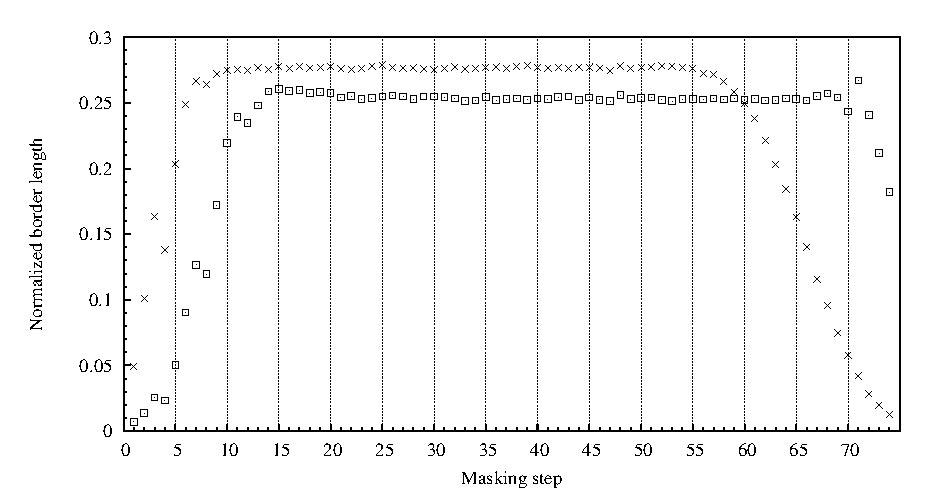
\includegraphics{merge/gplusmasks/bl}
\caption{\label{fig:gplus_blm}%
  Normalized border length per masking step of layouts produced by Greedy with
  $Q=20\,000$ ({\tiny $\times$}) and \Greedyplus\ with $Q=950$
  ({\tiny $\boxdot$}) for a $500\times 500$ chip with border length
  minimization. Both algorithms used $0$-threading and were followed by two
  passes of re-embedding optimization with Sequential.}
\end{figure}

\begin{table}[t!]\centering
\caption{\label{tab:gplus_reptx}
  Normalized border length (NBL) of layouts produced by Row-Epitaxial and
  \Greedyplus\ (both with $0$-threading) on random chips in approximately the
  same amount of time. (total time in minutes including two passes of Sequential
  re-embedding optimization). The relative difference in NBL and time between
  the two approaches is shown in percentage.}
\footnotesize{
\begin{tabular}{crrrlrrrlrr}
\vspace{1pt}
                & \multicolumn{3}{c}{Row-Epitaxial and Sequential} & & \multicolumn{3}{c}{\Greedyplus\ and Sequential} & & \multicolumn{2}{c}{Relative} \\ \cline{2-4} \cline{6-8} \cline{10-11}
\vspace{1pt}
Dim.            & Q       & NBL     &  Time & & Q      & NBL     & Time & & NBL       & Time \\
\hline
$300\times 300$ & 10\,000 & 18.0524 &   4.3 & &    300 & {\bf 17.9807} &  4.2 & & $-0.40\%$ &  $-1.24\%$ \\
                & 20\,000 & 17.9430 &   9.5 & &    700 & {\bf 17.6746} &  9.2 & & $-1.50\%$ &  $-2.85\%$ \\
\hline
$500\times 500$ & 10\,000 & 17.3584 &  16.0 & &    450 & {\bf 17.2216} & 16.0 & & $-0.79\%$ &  $-0.40\%$ \\
                & 20\,000 & 17.2502 &  34.7 & &    950 & {\bf 16.9382} & 30.4 & & $-1.81\%$ & $-12.51\%$ \\
\hline
$800\times 800$ & 10\,000 & 16.7176 &  45.6 & &    500 & {\bf 16.6549} & 41.7 & & $-0.38\%$ &  $-8.51\%$ \\
                & 20\,000 & 16.6012 & 100.1 & & 1\,130 & {\bf 16.3175} & 97.7 & & $-1.71\%$ &  $-2.41\%$ \\
\hline
\end{tabular}}
\end{table}

One advantage of \Greedyplus\ is that, unlike Greedy, it is not influenced by
the initial embeddings of the probes. Figure \ref{fig:gplus_blm} shows the
normalized border length of layouts produced by Greedy and \Greedyplus\ with
border length minimization for a selected $500\times 500$ chip with equivalent
numbers $Q$ of candidates per spot (in accordance with Table
\ref{tab:greedycomp_bl}). Because the probes were initially left-most embedded,
Greedy produced a layout in which the border conflicts are concentrated between
steps 7 and 58; starting on step 59, the normalized border length drops steadily
as the embeddings reach their last productive steps. In contrast, \Greedyplus\
produces a layout with a more uniform distribution of conflicts in the final
synthesis steps. In both cases the first masks have relatively few conflicts as
a result of lexicographically sorting the probes. A representation of selected
masks for the layout produced by \Greedyplus\ is shown in Figure
\ref{fig:gplus-bl_masks}. Layers of masked and unmasked regions in masks
$M_1 \dots M_9$ are similar to the ones shown in Figure
\ref{fig:greedy-bl_masks}, although the masks produced by Greedy are
``noisier''. The normalized border length of these layouts are $17.3182$
(Greedy) and $16.9451$ (\Greedyplus).

\begin{figure}[p]\centering
%%
\begin{picture}(435,567)\footnotesize{
\put( -2,439){\makebox(145,128){
\includegraphics{merge/gplusmasks/mask01}}}
\put(147,439){\makebox(145,128){
\includegraphics{merge/gplusmasks/mask02}}}
\put(292,439){\makebox(145,128){
\includegraphics{merge/gplusmasks/mask03}}}
\put( -2,429){\makebox(145, 10){$M_1$}}
\put(147,429){\makebox(145, 10){$M_2$}}
\put(292,429){\makebox(145, 10){$M_3$}}
\put( -2,296){\makebox(145,128){
\includegraphics{merge/gplusmasks/mask04}}}
\put(147,296){\makebox(145,128){
\includegraphics{merge/gplusmasks/mask05}}}
\put(292,296){\makebox(145,128){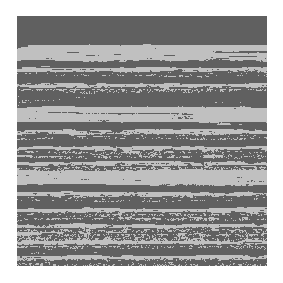
\includegraphics{merge/gplusmasks/mask06}}}
\put( -2,286){\makebox(145, 10){$M_4$}}
\put(147,286){\makebox(145, 10){$M_5$}}
\put(292,286){\makebox(145, 10){$M_6$}}
\put( -2,153){\makebox(145,128){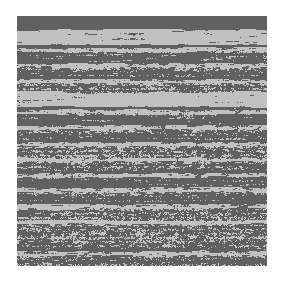
\includegraphics{merge/gplusmasks/mask07}}}
\put(147,153){\makebox(145,128){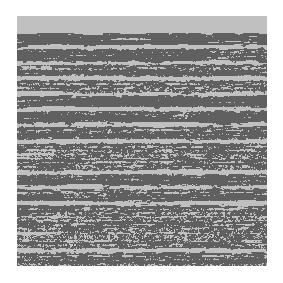
\includegraphics{merge/gplusmasks/mask08}}}
\put(292,153){\makebox(145,128){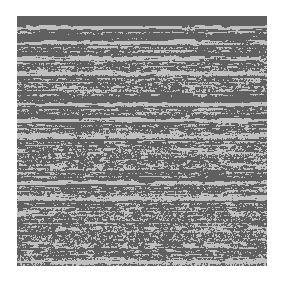
\includegraphics{merge/gplusmasks/mask09}}}
\put( -2,143){\makebox(145, 10){$M_7$}}
\put(147,143){\makebox(145, 10){$M_8$}}
\put(292,143){\makebox(145, 10){$M_9$}}
\put( -2, 10){\makebox(145,128){
\includegraphics{merge/gplusmasks/mask62}}}
\put(147, 10){\makebox(145,128){
\includegraphics{merge/gplusmasks/mask70}}}
\put(292, 10){\makebox(145,128){
\includegraphics{merge/gplusmasks/mask74}}}
\put( -2,  0){\makebox(145, 10){$M_{62}$}}
\put(147,  0){\makebox(145, 10){$M_{70}$}}
\put(292,  0){\makebox(145, 10){$M_{74}$}}
}\end{picture}
%%
\caption{\label{fig:gplus-bl_masks}%
  Selected masks generated by \Greedyplus\ with border length minimization for a
  $500\times 500$ chip with 25-mer probes embedded in the standard Affymetrix
  deposition sequence. Unmasked (masked) spots are represented by light (dark)
  dots.}
\end{figure}

Finally, we also compare \Greedyplus\ with Row-Epitaxial (Section
\ref{sec:placement_reptx}), which, in terms of border length minimization,
achieves results comparable to Greedy in less time. Table \ref{tab:gplus_reptx}
shows that \Greedyplus\ also outperforms Row-Epitaxial in the same amount of
time (or less). The larger values of $Q$ are used, the greater is the advantage
of \Greedyplus. According to the results of Table \ref{tab:greedyplus_nbl}, the
difference in NBL between \Greedyplus\ and Row-Epitaxial could be even greater
if the former used higher $k$-threading amplitudes.

%%%%%%%%%%%%%%%%%%%%%%%%%%%%%%%%%%%%%%%%%%%%%%%%%%%%%%%%%%%%%%%%%%%%%%%%%%%%%%%%
\section{Summary}
\label{sec:merge_summary}

We have presented a new placement algorithm, called \Greedyplus, that for the
first time places and re-embeds the probes simultaneously. Our results have
shown that \Greedyplus\ outperforms the previously best placement algorithms ---
Row-Epitaxial for border length minimization and Greedy for conflict index
minimization. In terms of CIM, Greedy produces better results when time is
limited but, otherwise, \Greedyplus\ should be the placement algorithm of
choice. In fact, \Greedyplus\ achieves similar results to Greedy by examining
fewer probe candidates per spot and, for this reason, it has the potential for
producing better layouts.

\subsection{Future work}

The fact that \Greedyplus\ does not outperform Greedy so easily in terms of CIM
as it does in terms of BLM could be explained by the fact that probes are sorted
lexicographically, which increases the chances of finding candidates that have
similar prefixes but not good ``matches'' for the middle part of the embeddings.
Greedy has an advantage since it looks at more candidates in the
lexicographically sorted list of probes. One possibility that could improve the
results of \Greedyplus\ is to sort the list of probes with an emphasis on the
middle bases. Although this is technically possible, with our current
implementation of OSPE it would result in an increase in running time because
consecutive candidates would then be unlikely to have a common prefix, requiring
the dynamic programming matrix to be entirely re-computed for each probe
considered. We leave as an open problem the question of finding an ordering of
the probes with an emphasis on the middle bases and an implementation of OSPE in
such a way that consective candidates can be examined quickly by skipping the
computation of identical rows of the matrix.

%%%%%%%%%%%%%%%%%%%%%%%%%%%%%%%%%%%%%%%%%%%%%%%%%%%%%%%%%%%%%%%%%%%%%%%%%%%%%%%%
\chapter{Analysis of Affymetrix Microarrays}
\label{ch:affy}
%%%%%%%%%%%%%%%%%%%%%%%%%%%%%%%%%%%%%%%%%%%%%%%%%%%%%%%%%%%%%%%%%%%%%%%%%%%%%%%%

Affymetrix GeneChip arrays are considered the industry standard in terms of
high-density oligonucleotide microarrays. In this chapter, we analyze the layout
of several GeneChip arrays with respect to the quality measures defined in
Chapter \ref{ch:mlp}, i.e., border length and conflict index. We then use some
of the algorithms presented in previous chapters to create alternative layouts
for two commercially available microarrays.

%%%%%%%%%%%%%%%%%%%%%%%%%%%%%%%%%%%%%%%%%%%%%%%%%%%%%%%%%%%%%%%%%%%%%%%%%%%%%%%%
\section{Introduction}
\label{sec:affy_intro}

We obtained the specification of several GeneChip arrays containing the list of
probe sequences and their positions on the chip from Affymetrix's web
site\footnote{\url{http://www.affymetrix.com/support/technical/byproduct.affx?cat=arrays}}.
As discussed below, we have to make a few assumptions because some details such
as the deposition sequence used to synthesize the probes, the probe embeddings,
and the contents of ``special'' spots are not publicly available.

Some of the special spots are used to help the mechanical alignment of the chip
with the scanner that captures the image with the hybridization signals. Others
contain \emph{quality control probes} used to detect failures during the
production of the chip \citep{Affymetrix2002,Hubbell1999a}. Not knowing the
contents of these special spots did not interfere with our analysis because, in
all arrays we examined, they amount to at most $1.22\%$ of the total number of
spots.

What could interfere with our analysis is the fact that some arrays have a
significant number of empty spots (as much as $11.94\%$ on the Chicken Genome
array). The physical location of some empty spots suggest that they might be
used as ``spacers'' to separate regions of the chip. Others might be empty
simply because the number of spots exceeds the number of probes. A high number
of empty spots result in a relatively low normalized border length (as defined
in Section \ref{sec:mlp_bl_vs_ci}) since we divide the total number of border
conflicts by the number of internal borders of the chip (an empty spot
contributes to the number of internal borders but obviously not to the number of
border conflicts). Thus, to better compare chips with different amounts of empty
spots we also use the \emph{average number of border conflicts per probe},
defined as the total border length divided by the number of probes. As we shall
see, an array with many empty spots might still have an advantage depending on
how the empty spots are distributed on the chip.

It has been reported that a fixed 74-step deposition sequence is used by
Affymetrix \citep{Kahng2004}. An analysis with the algorithms presented in
Chapter \ref{ch:scs} revealed that all GeneChip arrays, regardless of their
size, can be synthesized in $N=(\Seq{TGCA})^{18}\Seq{TG}$, i.e., $18.5$ cycles
of \Seq{TGCA}, and that a shorter deposition sequence is indeed unlikely. This
suggests that only sub-sequences of this particular deposition sequence can be
used as probes on Affymetrix chips. In principle, this should not be a problem
as this sequence covers about $98.45\%$ of all 25-mers \citep{Rahmann2006}.

\begin{figure}[t]\centering
\begin{tabular}{lc}
$N$              & \footnotesize{\tt{\verb|TGCATGCATGCATGCATGCATGCATGCATGCATGCATGCATGCATGCATGCATGCATGCATGCATGCATGCATG|}} \\
\hline
$\eps_p$         & \footnotesize{\tt{\verb| G AT   TG A G A   A  C   C  GCA G  T  A  C  G A  C   C   C  G  T         |}} \\
$\eps_{\bar{p}}$ & \footnotesize{\tt{\verb| G AT   TG A G A   A  C   C  G   G A G  T  A  C  G A  C   C   C  G  T     |}} \\
                 & \footnotesize{\tt{\verb|                              ++   +++ ++ ++ +++ +++         ++ ++  +     |}} \\
\hline
$\eps_p$         & \footnotesize{\tt{\verb| G AT   TG A G A   A  C   C  GC    A G  T  A  C  G A  C   C   C  G  T     |}} \\
$\eps_{\bar{p}}$ & \footnotesize{\tt{\verb| G AT   TG A G A   A  C   C  G   G A G  T  A  C  G A  C   C   C  G  T     |}} \\
                 & \footnotesize{\tt{\verb|                              +  +                                        |}} \\
\hline
\end{tabular}
\caption{\label{fig:pairwise_leftmost}%
  Left-most (above) and pair-wise left-most (below) embeddings $\eps_p$ and
  $\eps_{\bar{p}}$ of perfect match (PM) and mismatch (MM) probes
  $p=\Seq{GATTGAGAACCGCAGTACGACCCGT}$ and
  $\bar{p}=\Seq{GATTGAGAACCGGAGTACGACCCGT}$, respectively, in the standard
  Affymetrix deposition sequence $N=(\Seq{TGCA})^{18}\Seq{TG}$. Conflicts
  between the embeddings are highlighted with plus signs (\small{\tt{+}})
  in the corresponding synthesis steps.}
\end{figure}

Probes of GeneChip arrays always appear in pairs: the perfect match (PM), which
perfectly matches its target sequence, and the mismatch (MM) probe, which is
used to quantify cross-hybridizations and unpredictable background signal
variations \citep{Affymetrix2001}. The MM probe is a copy of the PM probe except
for the middle base (position 13 of the 25-mer), which is exchanged with its
Watson-Crick complement. The layout of GeneChip arrays alternate rows of PM
probes with rows of MM probes in such a way that probes of a pair are always
adjacent on the chip. Moreover, PM and MM probes are \emph{pair-wise left-most
embedded} \citep{Kahng2004}. Informally, a pair-wise left-most embedding is
obtained from left-most embeddings by shifting the second half of one embedding
to the right until the two embeddings are ``aligned'' in the synthesis steps
that follow the mismatched middle bases (Figure \ref{fig:pairwise_leftmost}).
This approach reduces border conflicts between the probes of a pair, although it
leaves a conflict in the steps that add the middle bases.

The fact that probes must appear in pairs restricts even more which sequences
can be used as probes on GeneChip arrays because both PM and MM probes must
``fit'' in the deposition sequence. For example, although
$p=\Seq{CGTAGGTACGTTATAAGTCACTAAA}$ has an embeddeding in
$N=(\Seq{TGCA})^{18}\Seq{TG}$, it cannot be used as a probe because its
corresponding mismatch probe $\bar{p}=\Seq{CGTAGGTACGTTTTAAGTCACTAAA}$ cannot be
embedded in $N$, as shown below.

\begin{tabular}{lc}
$N$              & \footnotesize{\tt{\verb|TGCATGCATGCATGCATGCATGCATGCATGCATGCATGCATGCATGCATGCATGCATGCATGCATGCATGCATG  |}} \\
\hline
$\eps_p$         & \footnotesize{\tt{\verb|  C  G  T  A G   G  T  A  C  G  T   T  AT  A   A G  T CA  C T  A   A   A    |}} \\
$\eps_{\bar{p}}$ & \footnotesize{\tt{\verb|  C  G  T  A G   G  T  A  C  G  T   T   T   T  A   A G  T CA  C T  A   A   A|}} \\
\hline
\end{tabular}

%%%%%%%%%%%%%%%%%%%%%%%%%%%%%%%%%%%%%%%%%%%%%%%%%%%%%%%%%%%%%%%%%%%%%%%%%%%%%%%%
\section{Layout Analysis}
\label{sec:affy_analysis}

\begin{figure}[t]\centering
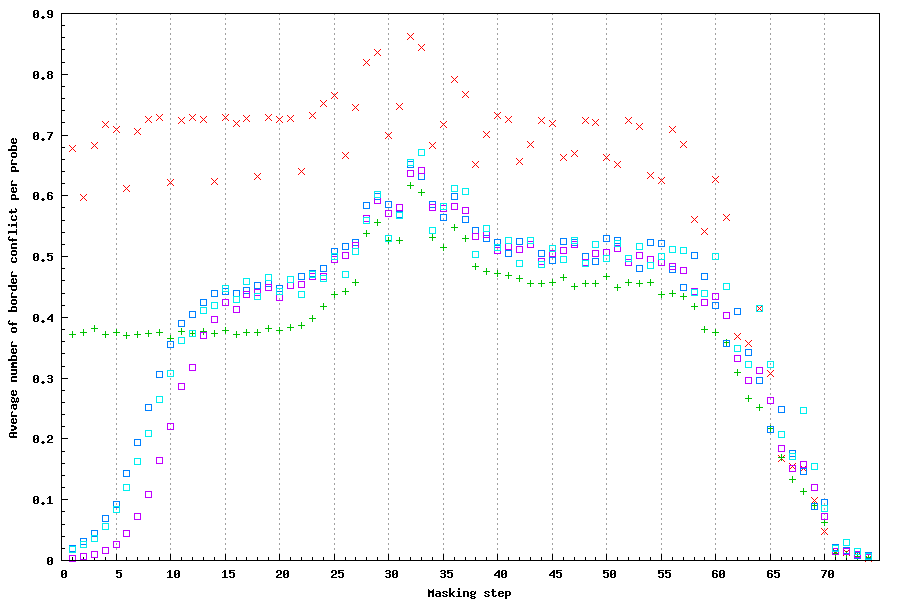
\includegraphics{affy/genechip/affy_blm}
\caption{\label{fig:affy_blm}%
  Average number of border conflicts per probe per masking step (on the left
  y-axis) of three GeneChip arrays, assuming pair-wise left-most embeddings:
  Yeast Genome S98 ({\scriptsize $\times$}), Human Genome U95A2 ({\tiny $+$}),
  and E.\ coli Genome 2.0 ({\tiny $\boxdot$}). The number of middle bases
  synthesized at each step on the E.\ coli Genome 2.0 is shown in boxes (on the
  right y-axis).}
\end{figure}

Figure \ref{fig:affy_blm} shows the average number border conflicts per probe
per masking step of three GeneChip arrays. We assume that the probes are
pair-wise left-most embedded in $N=(\Seq{TGCA})^{18}\Seq{TG}$, and we consider
all spots whose contents are not available as empty spots. In all chips we
analyzed, the number of border conflicts are higher in the steps that add the
middle bases, a result of placing PM and MM probes in adjacent spots. The Yeast
Genome S98 array has the worst layout in terms of border conflicts and most of
the earlier GeneChip arrays such as the E.\ coli Antisense Genome have similar
levels of conflicts. The layout of the Human Genome U95A2 array has signficantly
less border conflicts than the Yeast array, suggesting that it was designed with
a better placement strategy. The curve of the E.\ coli Genome 2.0 array, with
very low levels of conflicts in the first 10 masks, is typical of the latest
generation of GeneChip arrays, including the Chicken Genome and the Wheat Genome
(one of the largest GeneChip arrays currently available with
$1\,164\times 1\,164$ spots), and suggest yet another placement strategy.

Figure \ref{fig:ecoli_masks} shows a representation of selected masks for the
E.\ coli Genome 2.0. The low levels of conflicts in the first synthesis steps
are a result of the pattern of masked and unmasked layers that can be seen in
masks $M_1$ to $M_9$. This pattern is similar to the ones produced by Greedy
(Figure \ref{fig:greedy-bl_masks}) and \Greedyplus\ (Figure
\ref{fig:gplus-bl_masks}). A more careful examination, however, reveals that the
layers are arranged in a way that resembles the Gray-code--based arrangement
employed by 1-Dimensional Partitioning (Figure \ref{fig:1dpart}). This does not
necessarily mean that the layout was produced by such a partitioning. In fact, a
similar effect could be produced by a placement algorithm such as Greedy or
\Greedyplus\ if the probes were ordered in such a way that a prefix of their
binary embeddings formed an approximation of a Gray code.

\begin{figure}[p]\centering
%%
\begin{picture}(435,567)\footnotesize{
\put( -2,439){\makebox(145,128){
\includegraphics{affy/genechip/mask01}}}
\put(147,439){\makebox(145,128){
\includegraphics{affy/genechip/mask02}}}
\put(292,439){\makebox(145,128){
\includegraphics{affy/genechip/mask03}}}
\put( -2,429){\makebox(145, 10){$M_1$}}
\put(147,429){\makebox(145, 10){$M_2$}}
\put(292,429){\makebox(145, 10){$M_3$}}
\put( -2,296){\makebox(145,128){\includegraphics{affy/genechip/mask04}}}
\put(147,296){\makebox(145,128){\includegraphics{affy/genechip/mask05}}}
\put(292,296){\makebox(145,128){\includegraphics{affy/genechip/mask06}}}
\put( -2,286){\makebox(145, 10){$M_4$}}
\put(147,286){\makebox(145, 10){$M_5$}}
\put(292,286){\makebox(145, 10){$M_6$}}
\put( -2,153){\makebox(145,128){\includegraphics{affy/genechip/mask07}}}
\put(147,153){\makebox(145,128){\includegraphics{affy/genechip/mask08}}}
\put(292,153){\makebox(145,128){\includegraphics{affy/genechip/mask09}}}
\put( -2,143){\makebox(145, 10){$M_7$}}
\put(147,143){\makebox(145, 10){$M_8$}}
\put(292,143){\makebox(145, 10){$M_9$}}
\put( -2, 10){\makebox(145,128){\includegraphics{affy/genechip/mask32}}}
\put(147, 10){\makebox(145,128){\includegraphics{affy/genechip/mask50}}}
\put(292, 10){\makebox(145,128){\includegraphics{affy/genechip/mask70}}}
\put( -2,  0){\makebox(145, 10){$M_{32}$}}
\put(147,  0){\makebox(145, 10){$M_{50}$}}
\put(292,  0){\makebox(145, 10){$M_{70}$}}
}\end{picture}
%%
\caption{\label{fig:ecoli_masks}%
  Selected masks of Affymetrix's E.\ coli Genome 2.0 GeneChip array, assuming
  pair-wise left-most embeddings. Unmasked (masked) spots are represented by
  light (dark) dots. White regions represent spots whose contents are not
  publicly available.}
\end{figure}

Table \ref{tab:genechip} confirms that the layout of the Human Genome U95A2
array is the best in terms of normalized border length and average conflict
index. This, however, has more to do with empty spots than with the placement
strategy as this chip has about $1.83\%$ of empty spots that are evenly
distributed on the chip surface (Figure \ref{fig:chipmaps}, left). In contrast,
the Chicken Genome array has an exceptionally high percentage of empty spots
($11.94\%$) that contribute to lower the normalized border length but that does
not result in a lower average number of border conflicts per probe in comparison
with the Human Genome array because the empty spots are concentrated in the
lower part of the chip (Figure \ref{fig:chipmaps}, right).

\begin{table}[t!]\centering
\caption{\label{tab:genechip}
  Average number of border conflicts per probe (ABC), normalized border length
  (NBL) and average conflict index (ACI) of selected GeneChip arrays (assuming
  pair-wise left-most embeddings). The dimension of the chip, the percentage of
  spots with unknown content and the percentage of empty spots are also shown.}
\footnotesize{
\begin{tabular}{lcrrrrr}
GeneChip Array            & Dimension             & Unknown  & Empty     & ABC     & NBL     & ACI \\
\hline
Yeast Genome S98          & $534\times 534$       & $1.22\%$ &  $1.70\%$ & 44.8168 & 21.7945 & 669.0663 \\
E.\ coli Antisense Genome & $544\times 544$       & $1.17\%$ &  $3.12\%$ & 43.3345 & 20.7772 & 663.7353 \\
Human Genome U95A2        & $640\times 640$       & $0.96\%$ &  $1.83\%$ & 28.2489 & 13.7517 & 510.3418 \\
E.\ coli Genome 2.0       & $478\times 478$       & $1.08\%$ &  $0.46\%$ & 29.2038 & 14.4079 & 550.2014 \\
Chicken Genome            & $984\times 984$       & $0.46\%$ & $11.94\%$ & 28.2087 & 12.3680 & 540.5022 \\
Wheat Genome              & $1\,164\times 1\,164$ & $0.38\%$ &  $0.08\%$ & 27.6569 & 13.7771 & 539.9632 \\
\hline
\end{tabular}}
\end{table}

GeneChip arrays exhibit relatively low levels of border conflicts when compared
to layouts produced by the best algorithms for random arrays of similar
dimensions. This can be explained by the fact that each probe has a nearly
identical copy next to it. Not surprisingly, these arrays have relatively high
average conflict indices when compared to random arrays because the conflicts
are concentrated on the synthesis steps that add the middle bases.

\begin{figure}[t]\centering
%%
\begin{picture}(435,225)
\put(  0, 15){\makebox(210,210){\includegraphics{affy/genechip/HGU95A2-S_affy_chipmap}}}
\put(210, 15){\makebox( 15,210){}}
\put(225, 15){\makebox(210,210){\includegraphics{affy/genechip/CHK-S_affy_chipmap}}}
\put(  0,  0){\makebox(210, 15){\footnotesize{Human Genome U95A2 ($640\times 640$)}}}
\put(210,  0){\makebox( 15, 15){}}
\put(225,  0){\makebox(210, 15){\footnotesize{Chicken Genome ($984\times 984$)}}}
\end{picture}
%%
\caption{\label{fig:chipmaps}%
  Distribution of empty spots on two GeneChip arrays. Chip dimensions are
  indicated in parenthesis (images were scaled differently). Non-empty spots are
  represented by dark dots. White dots represent empty spots or spots whose
  contents are not publicly available.}
\end{figure}

%%%%%%%%%%%%%%%%%%%%%%%%%%%%%%%%%%%%%%%%%%%%%%%%%%%%%%%%%%%%%%%%%%%%%%%%%%%%%%%%
\section{Alternative Layouts}
\label{sec:affy_alternative}

We used \Greedyplus\ (Chapter \ref{ch:merge}) and Sequential re-embedding
(Section \ref{sec:reembed_sequential}) to create alternative layouts for two of
the latest generation of GeneChip arrays: E.\ coli Genome 2.0 and Wheat Genome.
\Greedyplus\ was modified to avoid placing probes on special spots or empty
spots that we believe might have a function on the chip.

For each chip we run the algorithms with border length as well as conflict index
minimization. The main difference between our layouts and the original ones is
that we do not require the arrays to alternate rows of PM and MM probes; hence,
probes of a pair are not necessarily placed on adjacent spots. This is
especially helpful for conflict index minimization since it avoids conflicts in
the middle bases. With border length minimization, we observed that \Greedyplus\
placed between $90.70\%$ and $95.16\%$ of the PM probes adjacent to their
corresponding MM probes. With conflict index minimization, this rate dropped to
between $12.89\%$ and $21.25\%$.

Figure \ref{fig:alternative_ec2} shows the normalized border length per masking
step of the layout produced by \Greedyplus\ and Sequential for the E.\ coli
Genome 2.0 array in comparison with the original Affymetrix layout. For
comparison, we also show the result of running a ``pair-aware'' version of
Sequential on the original layout (this version ensures that the embeddings of
PM-MM pairs remain pair-wise ``aligned''). The normalized border length and
average conflict indices of these layouts are shown on Table
\ref{tab:alternative}, together with several layouts for the Wheat Genome array.
\Greedyplus\ with $Q=10$K produced a layout with $8.10\%$ less border conflicts
than the original layout for the E.\ coli array ($13.2406$ versus $14.4079$) in
$218.3$ minutes. With $Q=2$K, this difference was $7.15\%$, although that
required only $46.9$ minutes. For the Wheat array, \Greedyplus\ with $Q=2$K
generated a layout with $7.36\%$ less border conflicts than the original layout
($12.7622$ versus $13.3771$). It is not fair to compare the layouts in terms of
CIM since the original layouts were probably designed to minimize border
conflicts (and not conflict indices). Nevertheless, the results produced by
\Greedyplus\ and Sequential are comparable to the results on random chips
presented on Chapter \ref{ch:merge}.

\begin{table}[t!]\centering
\caption{\label{tab:alternative}
  Normalized border length (NBL) and average conflict index (ACI) of several
  layouts for the E.\ coli Genome 2.0 and Wheat Genome GeneChip arrays.
  \Greedyplus\ and Sequential run with border length and conflict index
  minimization (BLM and CIM, respectively) as indicated. \Greedyplus\ used
  $k$-threading with $k=5$ for BLM and $k=0$ for CIM. Running times are reported
  in minutes and include placement (\Greedyplus) and 2 passes of re-embedding
  optimization with Sequential.}
\footnotesize{
\begin{tabular}{llrrr}
Array & Layout                                                  & NBL     & ACI      & Time\\
\hline
E.\ coli 2.0 & Affymetrix with pair-wise left-most              & 14.4079 & 550.2014 & --- \\
             & Affymetrix after ``pair-aware'' Sequential (BLM) & 13.5005 & 541.0954 & --- \\
             & \Greedyplus\ with $Q=2$K and Sequential (BLM)    & 13.3774 & 529.8129 &  46.9 \\
             & \Greedyplus\ with $Q=10$K and Sequential (BLM)   & 13.2406 & 515.5917 & 218.3 \\
             & \Greedyplus\ with $Q=2$K and Sequential (CIM)    & 17.6935 & 394.9905 &  54.9 \\
             & \Greedyplus\ with $Q=10$K and Sequential (CIM)   & 17.5575 & 361.4418 & 225.7 \\
\hline
Wheat        & Affymetrix with pair-wise left-most              & 13.7771 & 539.9632 & --- \\
             & Affymetrix after ``pair-aware'' Sequential (BLM) & 12.9151 & 531.2692 & --- \\
             & \Greedyplus\ with $Q=2$K and Sequential (BLM)    & 12.7622 & 519.0869 & 279.2 \\
             & \Greedyplus\ with $Q=5$K and Sequential (BLM)    & 12.6670 & 511.7193 & 676.0 \\
             & \Greedyplus\ with $Q=2$K and Sequential (CIM)    & 17.1047 & 387.8430 & 322.7 \\
             & \Greedyplus\ with $Q=5$K and Sequential (CIM)    & 17.1144 & 366.6045 & 704.7 \\
\hline
\end{tabular}}
\end{table}

\begin{figure}[t]\centering
\includegraphics{affy/alternative/EC2}
\caption{\label{fig:alternative_ec2}%
  Normalized border length per masking step of several layouts for the E.\ coli
  Genome 2.0 GeneChip array: original Affymetrix layout with pair-wise left-most
  embeddings ({\tiny $\odot$}), original Affymetrix layout after running two
  passes of a ``pair-aware'' version of Sequential re-embedding ({\tiny $+$}),
  layout produced by \Greedyplus\ with $Q=10$K and Sequential with border length
  minimization ({\tiny $\boxdot$}), and layout produced by \Greedyplus\ with
  $Q=10$K and Sequential with conflict index minimization
  ({\scriptsize $\times$}).}
\end{figure}

%%%%%%%%%%%%%%%%%%%%%%%%%%%%%%%%%%%%%%%%%%%%%%%%%%%%%%%%%%%%%%%%%%%%%%%%%%%%%%%%
\section{Summary}
\label{sec:affy_summary}

We have analyzed the layout of several commercial microarrays with respect to
border length and conflict index. It is clear that placing perfect match (PM)
and mismatch (MM) probes on adjacent spots reduces the incidence of border
conflicts. However, this also has the disadvantage of concentrating the
conflicts on the synthesis steps that add the middle bases, precisely where the
probes are most likely to be damaged.

We have also showed that two algorithms presented in earlier chapters,
\Greedyplus\ and Sequential re-embedding, performed well on real microarrays,
including one of the largest GeneChip arrays available, producing layouts with
up to $8.10\%$ less border conflicts than the original layouts in reasonable
time, and layouts with average conflict index comparable to results on random
arrays. In general, we believe that the quality of currently available GeneChip
arrays can be significantly improved with respect to the problem of unintended
illumination.

%%%%%%%%%%%%%%%%%%%%%%%%%%%%%%%%%%%%%%%%%%%%%%%%%%%%%%%%%%%%%%%%%%%%%%%%%%%%%%%%
\chapter{Shortest Common Supersequence}
\label{ch:scs}
%%%%%%%%%%%%%%%%%%%%%%%%%%%%%%%%%%%%%%%%%%%%%%%%%%%%%%%%%%%%%%%%%%%%%%%%%%%%%%%%

\chapter{Discussion}
\label{ch:discussion}

This thesis makes several contributions to the field of....

We introduce the \emph{conflict index}...

In Chapter X we present a algorithm...

We are not aware of any previous work that combines placement and
re-embedding, even our results showed that such an approach has
obvious benefits...

We have surveyed algorithms for the microarray layout problem (MLP), divided
into placement, (re-)embedding, and partitioning algorithms.  Because of the
super-exponential number of possible layouts and the relation to the quadratic
assignment problem (QAP), we cannot expect to find optimal solutions. Indeed,
the algorithms we present are heuristics with an emphasis on good scalability
and ideally a user-controllable trade-off between running time and solution
quality, albeit without any known provable guarantees.

Among the presented approaches, two recent ones (Pivot Partitioning and
\Greedyplus) indicate that the traditional ``place first and then re-embed''
approach can be improved upon by merging the partitioning/placement and
(re-)embedding phases. Ongoing work will show the full potential of such
combined approaches.

As a suggestion for further work, we note the needed for improving
the selection of probe candidates considered for filling each spot. For
example, instead using a sorted list of probes, one could use a TSP tour
like the early algorithms described in Sec.~\ref{sec:placement_early}. However,
it is not clear if the more time-consuming TSP approach will pay off
(instead, we could use this extra time to look at more candidates).

An alternative that sounds interesting would be to build some kind of
``clustering'' of the probes, perhaps based on a graph or a tree, in such a
way that we can find similar probes more easily and spend time on candidates
that are more likely to produce less conflicts.

Question: why PM and MM probes are placed together and aligned except for the
middle base?

%%%%%%%%%%%%%%%%%%%%%%%%%%%%%%%%%%%%%%%%%%%%%%%%%%%%%%%%%%%%%%%%%%%%%%%%%
%% Bibliography
%%%%%%%%%%%%%%%%%%%%%%%%%%%%%%%%%%%%%%%%%%%%%%%%%%%%%%%%%%%%%%%%%%%%%%%%%
\bibliographystyle{abbrvnat}
\bibliography{diss}

%\cleardoublepage
%\part*{Appendix}
%\appendix
%\input{Software}

\end{document}

%%%%%%%%%%%%%%%%%%%%%%%%%%%%%%%%%%%%%%%%%%%%%%%%%%%%%%%%%%%%%%%%%%%%%%%%
